% Copyright � 2015 by James Dean Mathias
% All Rights Reserved

\documentclass[oneside, letterpapaer, openright]{book}

\usepackage[margin=3cm]{geometry}

\usepackage{hyperref}
\usepackage{listings}
\usepackage{xcolor}
\usepackage{caption}
\usepackage{graphicx}
\usepackage{mdframed}
\usepackage{float}
\usepackage{wallpaper}
\usepackage{tkz-graph}
\usepackage{tikz}
\usetikzlibrary{positioning}
\usetikzlibrary{shapes.geometric}
\usetikzlibrary{arrows}

\newcommand{\FigureCode}{Listing }
\lstnewenvironment{code}[1][] 
{
	%\minipage{\linewidth}
	\renewcommand{\lstlistingname}{\FigureCode}
	\lstset 
	{
		basicstyle=\small
		language=C++,
		backgroundcolor=\color{black!5}, % set backgroundcolor
		basicstyle=\small,% basic font setting
		showstringspaces=false,
		moredelim=**[is][\bfseries]{```}{```},
		%frame=single,
		%captionpos=b % Place the caption on the bottom				
		#1
	}
}
{
	%\endminipage
}

\newcommand{\FigureConsole}{Figure }
\lstnewenvironment{console}[1][] 
{
	%\minipage{\linewidth}
	\renewcommand{\lstlistingname}{\FigureConsole}
	\lstset 
	{
		basicstyle=\small
		backgroundcolor=\color{black!5}, % set backgroundcolor
		basicstyle=\small,% basic font setting
		showstringspaces=false,
		#1
	}
}
{
	%\endminipage
}

\newcommand{\FigureGeneral}{Figure }
\lstnewenvironment{general}[1][] 
{
	%\minipage{\linewidth}
	\renewcommand{\lstlistingname}{\FigureGeneral}
	\lstset 
	{
		basicstyle=\small
		backgroundcolor=\color{black!5}, % set backgroundcolor
		basicstyle=\small,% basic font setting
		showstringspaces=false,
		#1
	}
}
{
	%\endminipage
}

\DeclareCaptionFont{white}{\color{white}}
\DeclareCaptionFormat{listing}{\colorbox{gray}{\parbox{\textwidth}{#1#2#3}}}
\captionsetup[lstlisting]{format=listing,labelfont=white,textfont=white}

%\title{Developing Scalable Systems Using C++11}
%\title{A Practical Guide To Scalable Systems Using C++11}
\title{Scalable, Distributed, \& Fault-Tolerant Systems Using C++11}
\author{James Dean Mathias, Ph.D.}


% This is the 'less is more' chapter heading style
% Reference: http://texblog.org/2012/07/03/fancy-latex-chapter-styles/
\usepackage[T1]{fontenc}
\usepackage{color}
\usepackage{titlesec}
\definecolor{gray75}{gray}{0.75}
\newcommand{\hsp}{\hspace{20pt}}
\titleformat{\chapter}[hang]{\Huge\bfseries}{\thechapter\hsp\textcolor{gray75}{|}\hsp}{0pt}{\Huge\bfseries}

\begin{document}

	\ThisCenterWallPaper{1.0}{Images/MandelCover-3.png}
	\maketitle
	\clearpage
	
	\frontmatter
	\tableofcontents
	
	\mainmatter
	% Copyright � 2015 by James Dean Mathias
% All Rights Reserved

\chapter{Introduction}\label{chapter:overview}

The purpose of this book is to act as a resource for those interested in building scalable, distributed, and fault-tolerant systems using C++11 and the Boost C++ libraries. Each of these topics is covered in detail, along with working code that can be used as the basis for developing or extending your applications. The combination of the C++11 language enhancements and standard library additions have made cross platform, distributed systems programming more accessible than ever before. This is a practical guide that shows how to develop these systems using C++11, with support from the Boost C++ libraries; this is a code heavy book.

This book assumes a background in C++ programming, familarity with multi-threading, synchronization, and network programming concepts, but not necessarily mastery or other expertise with them. Exposure to the new features introduced with C++11 language and standard library is not assumed, therefore an introduction to relevant topics are covered in Chapter \ref{chapter:cpp11}. In particular, this includes lambda functions, along with the new threading and synchronization libraries. No background with Boost is assumed, an introduction to Boost and the relevant networking libraries is provided in Chapter \ref{chapter:networking}. Enough discussion is given and code provided to be reasonably accessible to a wide range of developers, from the relatively inexperienced all the way up to senior developers.

The overarching approach presented in this book is that of task/data decomposition, presented in the context of scalability, distribution, and fault-tolerance. There are a number of tecchnical implementation details that are necessary which can work to obscure the general simplicity of the overall approach. It is important to maintain focus while working through these technical details that fundamentally, the building block is that of identifying and developing tasks that can be computed in parallel. This is true regardless if the application is intended to run on a single computer with any number of processors and CPU cores, or as a distributed application running across a wide range of heterogenous systems.

This book takes something of a \textit{roll your own} approach to the construction of applications. It is recognized there are existing frameworks such as OpenMP\footnote{http://en.wikipedia.org/wiki/OpenMP}, MPI\footnote{http://en.wikipedia.org/wiki/Message\_Passing\_Interface}, and HTCondor\footnote{http://en.wikipedia.org/wiki/HTCondor} that can be used as building blocks to achieve similar results, however, those frameworks are not appropriate for all applications; this book does not present development approaches using such frameworks. There are any number of good reasons to choose those for an application, similarly there are any number of good reasons not to choose them. The techniques presented in this book may be considered at a lower level than those because much of the infrastructure is built from the ground up, but also simply a \textit{different} approach, with its own set of pros and cons, which are discussed throughout.

Existing applications benefit greatly from the approach presented in this book. It is likely easier to modify an application to incorporate the computing framework presented in this book versus changing the computing model over to something like MPI. Furthermore, not all computing environments are as controlled, or dedicated, as required for something like MPI. Your application may need to be delivered to dozens or thousands of customers, only some of which have the systems expertise or environment necessary to setup an MPI framework. The techniques presented in this book require zero configuration for single systems and trival configuration (command line parameters) for distributed applications, making such applications much more reasonable to deploy and deliver to customers.

\section{C++11 Features}

C++11 introduced a host of new language and standard library features. While C++ is never going to be considered a syntactically \textit{simple} language, many of the new language features help to reduce some of the syntactic complexity. Additionally, the standard library has adopted a number of libraries from Boost which support the writing of cross-platform and multi-threaded applications. A full chapter is dedicated to introducing the new capabilities that are specifically relevant to the construction of scalable, distributed, and fault-tolerant systems as presented in this book.

The following language and standard library features are discussed in Chapter \ref{chapter:cpp11}:

\begin{itemize}
	\item \texttt{auto} Keyword
	\item \texttt{decltype} operator
	\item \texttt{nullptr} Constant
	\item Range-based for Loop
	\item Smart Pointers
	\item Lambdas
	\item Threading \& Synchronization
\end{itemize}

Each of these topics is discussed in detail and presented with working code samples to demonstrate their use.

\section{Boost C++ Libraries}

Chapter \ref{chapter:networking} provides an introduction to the Boost C++ libraries, which provides the basis for the networking framework used by much of the code presented in this book. Boost.Asio is the primary library that is covered. It provides a high-level approach to interprocess communication (i.e., networking), along with some key capabilities in support of threading, thread pools, and synchronization with respect to interprocess communication.

The following topics from the Boost.Asio library are covered in Chapter \ref{chapter:networking}:

\begin{itemize}
  \item Introduction to Boost.Asio
  \item The \texttt{io\_service}
  \item The \texttt{io\_service} Queue
  \item Thread Pools on an \texttt{io\_service}
  \item Strands
  \item Buffers
  \item Socket Connections
  \item Socket Communication
  \item Multi-threading \& Sockets
\end{itemize}

\section{Scalable Systems}

In the context of this book a \textit{scalable} system is used to describe an application that scales to fully utilize the capabilities of a single computer or device. Generally speaking \textit{scalable} applies to all kinds of applications, whether they run on a single computer or on a large distributed computing environment. Because this book builds towards full distributed and fault-tolerant systems, it is necessary to reduce the scope of the term to mean only a single computing device.

Three chapters are devoted to the topic of scalable systems, two for distributed systems, and only a single for fault-tolerance, with one more chapter extending the fault-tolerance framework capabilities. The reason for this is that scalability is the building block upon which the other systems are built. The next major building block is the distribured framework. Once the scalable and distributed infrastructure is in place, the most complex parts of the system are complete, allowing the fault-tolerant component to come along as a modest update.

Scalable systems begin with identifying computing tasks that can be computed in parallel. Chapter \ref{chapter:scalable-task-based} starts the discussion by showing how to create an application that can take small computing tasks and spread them over any number of available CPU cores on a system. Often times applications have need for associating priority with tasks, some need to be done as soon as possible, others can tolerate being delayed. Chapter \ref{chapter:scalable-priority} takes on the challenge of creating a system that provides for application level control of task priority. Finally, it is often the case that some tasks must wait for others to complete before they can be computed, causing even more complexity in the underlying task distribution logic. Chapter \ref{chapter:scalable-dag} tackles the complex subject of providing for dependencies among computing tasks.

The work done in the initial chapter on scalable computing, Chapter \ref{chapter:scalable-task-based}, in building a framework that performs computations through a task-based approach is the most important. Everything else is just different ways of managing the order, distribution, and collection of the results from the tasks. Priority and dependencies affect the ordering of when and how the tasks are computed, whereas distribution changes the physical device to which computing resource a task is directed, and fault-tolerance decides how to handle tasks that are in process when their computing resource fails. Everything revolves around having a task-based computing framework, with that in place, the other capabilities become quite reasonable to provide.

\section{Distributed Systems}

This book uses the term \textit{distributed system} to mean any two or more connected computing devices, which may be homogenous (same capabilities) or heterogeneous (different capabilities). When used in combination with \textit{scalable} to describe an application, it means an application that scales to fully utilize the capabilities of all the connected systems. Furthermore, the intention is that the application scales across the distributed environment without requiring it to be rebuilt, it dynamically adapts to fully utilize the system's resources.

\section{Fault-Tolerant Systems}

An easily overlooked component of distributed systems is \textit{fault-tolerance}. Fault-tolerance indicates an ability for an application to recover gracefully from a failure or error condition. The kind of fault-tolerance presented in this book is with respect to network and computing device failures. The goal is to build a system that continues correct operation in the face of an unreliable network or computing environment. Solving for one of these errors, solves both problems. As far as an application is concerned, the failure of either a network connection to a computing device, or the failure of the computing device itself looks the same and has the same result, the computing resource is no longer available. Therefore, a solution to one, is a solution to both.

Fault-tolerance only means \textit{tolerant}, not \textit{immune}, to failures. There are any number of different failure scenarios an application may face, both internal and external. The degree to which fault-tolerance is supported depends upon the application need, the complexity of providing that support, and ultimately the cost. A speadsheet has different fault-tolerant requirements versus a multi-player game versus the software running an inter-planetary probe, with each having different risks and costs.

A further benefit of building this kind of fault-tolerance is the ability for the application to dynamically scale, up or down, as computing resources come and go. Perhaps your application utilizes unused computing resources when employees leave for the day. By allowing for fault-tolerance an application can dynamically increase resource utilization when a computing resource becomes available, and similarly dynamically decrease resource utilization as appropriate, all while still providing correct operation.

One goal for this book is to show that it is relatively straightforward to add a fairly robust fault-tolerant capability to an application, when the proper underlying framework is provided. By building upon the task-based framework developed in the scalable and distributed chapters of the book, fault-tolerance readily fits into the model and is implemented with only modest code changes.

\section{Performance}

The framework algorithms in the code presented throughout the book are written to be approachable and generalized, with performance a secondary consideration. With respect to performance, they must be evaluated in the context of overall system performance. When the applications presented in this book are profiled, over 97\% of the time is spent doing computational tasks, rather than framework or synchronization. While more performance improvements may be made, they provide no meaningful impact with respect to overall system performance.

\section{Source Code}

A large number of working demonstration programs are provided as part of this book. To a great extent, the chapter discussions are oriented around explaining sections of code from these demonstration programs. In particular, the core chapters on scalability, distributed systems, and fault-tolerant systems, are based around different implementations of an interactive Mandelbrot visualization application. The full source code for each revision is provided as part of this book, which includes each different building block framework. The frameworks from these programs can be used as the basis for developing a new application of your own, or for integration into an existing system.

The code presented within the pages of the book sometimes differs from that found in the downloaded source code. In order to fit code within the pages of the book, the formatting is often changed from what I do in a code editor; it is not how I prefer to format the code, but it is the limitation of the book format. Sometimes the code snippits are changed slightly to eliminate statements that create unnecessary noise as part of the discussion. Almost all comments are removed from the source listings, while the downloaded code is filled with comments. Finally, I expect to continue to make small improvements to the code after publication of the book.

\section{Looking Forward}

This book is only the first step in the evolution of an even more sophisticated system I am working towards. The following are topics that I intend to tackle in revisions to this book and another book that follows on from this one:

\begin{itemize}
  	\item Finish separation of framework from application code
	\item Google Protocol Buffers
	\item Authentication and encryption
	\item Reporting of task status for better fault detection
	\item Task cancellation
	\item Overcome single point of failure
\end{itemize}

The first change I'd like to make is to fully separate underlying framework from the application code. Currently there are bits of the framework in the application code, such as the setup of the networking and handling of the result messages. This needs to get cleaned up and fully separated from the application code.

The next change is to move away from the custom, ad-hoc, message encoding scheme and replace it with Google Protocol Buffers\footnote{https://github.com/google/protobuf}. The technique presented in this revision of the book is well and good, but has some compromises. Part of the purpose in replacing it is that it will force me to create a better separation between task and messaging code. It also provides the benefit of a significantly more robust message definition scheme, one that can stand the test of time as an application grows. 

An enhancement that goes along with replacing the messaging scheme is to introduce authentication and encryption. I have a long term eye towards the ability for this framework to be utilized over the Internet. Because of this, it makes sense to authenticate and encrypt all networking traffic to help prevent hacking.

Another area that needs to be addressed is a robust way to handle knowing when a server has failed and a task (or tasks) should be distributed elsewhere. The current mechanism is to define a timeout, which is difficult to do at coding time, given that different computers will execute the task at different rates. Therefore a new task computation status reporting scheme is required, one that has compute servers report at expected intervals the status of a task execution. This can then form the basis for better fault detection and recovery.

Related to task status and fault detection is the ability to cancel a task, or group of tasks, after having been sent for computation. There are several reasons for doing this. The first is that the operator of an application may decide some long-running task (or tasks) are no longer needed, and they should be immediately cancelled, making the resources they are currently consuming available for other tasks. Another reason is to allow for a more rapid shutdown. The current system requires that any tasks currently running at a compute server must complete before it will finish responding to a termination signal.

One of the biggest issues to overcome is the single point of failure that exists with having only one client. In the design presented throughout this book, if the client fails, the entire system goes down. My eventual design removes the problem of having a single client, allowing for any number of clients, and allowing for any (or all) of them to fail, but leaving the server framework intact and available as new clients connect.

\section{Acknowledgements}

I'd like to thank the following for helping with comments that have aided in improving the text: Chad Knight, Seth Humphries, Matt Burnham, Chris Heaps, and Scott Cannon.

	% Copyright � 2015 by James Dean Mathias
% All Rights Reserved

\chapter{Relevant C++11 Features}\label{chapter:cpp11}

C++11 was adopted in August of 2011 and introduces a host of new language and standard library features. The language was enhanced with several features that simpify the way code is written, making it possible to write more concise code, at the same time, making it more understandable. With respect to new language features, of particular note are the \textit{auto} keyword, the range-based for loop, and lambdas. The standard library was significantly enhanced by adopting a number of libraries from Boost (\href{http://www.boost.org}{http://www.boost.org}), along with adding a few new pieces. Specifically the threading and synchronization libraries enable a single C++ code-base that compiles and executes on a wide number of platforms. This chapter discusses the C++ features introduced with C++11 that are used throughout this book; it is not an exhaustive review of all new C++11 language and standard library features.

\section{\texttt{auto} Keyword}\label{chapter:cpp11:auto}

The \texttt{auto} keyword is used to instruct the compiler to infer the type for a variable (or constant if you like). Even though the developer does not declare the type, the type is still known, by inference, to the compiler and while the program is compiled; it is not a dynamic or variant type.

A trivial usage of \texttt{auto} is for primitive types, such as \texttt{int}s and \texttt{float}s. Examples of these are shown in \FigureCode \ref{chapter:cpp11:auto:trivial}.

\begin{code}[caption={Trivial \texttt{auto}}, label=chapter:cpp11:auto:trivial]
auto intValue = 10;
auto floatValue = 3.14f;
\end{code}

Another case for using the \texttt{auto} keyword is when using iterators. It is generally cumbersome and mistake-prone to write out the full type for an iterator, the \texttt{auto} keyword eases this burden. Inferring the type of an iterator is shown in \FigureCode \ref{chapter:cpp11:auto:iterator}.

\begin{code}[caption={Inferred Iterator}, label=chapter:cpp11:auto:iterator]
std::unordered_map<std::string, std::uint_32> cityPopulation;
... // cityPopulation is initialized here

auto myHome = cityPopulation.find("My Home");
\end{code}

Without the \texttt{auto} keyword, the \texttt{.find} statment would have to look like \FigureCode \ref{chapter:cpp11:auto:typed-iterator}.

\begin{code}[caption={Iterator Type}, label=chapter:cpp11:auto:typed-iterator]
std::unordered_map<std::string, std::uint32_t>::iterator 
  myHome = cityPopulation.find("My Home");
\end{code}

There is no universal guiding principle for when to use \texttt{auto} versus writing the type (e.g., \texttt{uint16\_t}); although Scott Meyers might disagree. You'll have to develop your own preference for the most appropriate usage; the code presented in the book demonstrates my preference at the time of writing.

\section{\texttt{decltype} Operator}\label{chapter:cpp11::decltype}

The \texttt{decltype} keyword is an operator that extracts the type of a variable or expression. This operator instructs the  compiler to take the type of the variable or expression and use it as the type for the specified identifier. \FigureCode \ref{chapter:cpp11:decltype:trivial} shows an example of a trival usage of \texttt{decltype}.

\begin{code}[caption={Trivial \texttt{decltype}}, label=chapter:cpp11:decltype:trivial]
int source = 10;
decltype(source) scaled = source * 4;
\end{code}

The sample code provided in \FigureCode \ref{chapter:cpp11:decltype:template} shows its utility with template types. The class \texttt{EightBitArray} is templated on the data type of an array that has a fixed size off 256 entries (8 bits). The variable \texttt{source} requires a type declaration, whereas \texttt{destination}'s type is based upon the type of the variable \texttt{source}.

\begin{code}[caption={Templates \& \texttt{decltype}}, label=chapter:cpp11:decltype:template]
template <typename T>
class EightBitArray
{
public:
  T& operator[](uint8_t index) { return m_array[index]; }

private:
  std::array<T, 256> m_array;
};

int main()
{
  EightBitArray<double> source;
  decltype(source) destination;

  ... Do something interesting with the arrays ...

  return 0;
}
\end{code}

Without the context of a larger application it is difficult to demonstrate \texttt{decltype}'s effective use, but there are good uses that help clean up some otherwise clumsy syntax. The way that I've found to use \texttt{decltype} is to ensure a set of related types are all the same. The initial type is specified, then all other variables, class members, or parameters are defined using \texttt{decltype}. In this way, when the original type is changed, all the other types are guaranteed to change at the same time, without having to go through all the code, potentially making a mistake.

\section{\texttt{nullptr} Constant}\label{chapter:cpp11:nullptr}

C++11 introduces a \texttt{nullptr} constant that is intended for use with pointer types, versus the old C and C++ techniques of \texttt{NULL} and \texttt{0}. Having the \texttt{nullptr} constant prevents ambiguity with the integral values of \texttt{NULL} and \texttt{0}. Its use is quite simple, as demonstrated in \FigureCode \ref{chapter:cpp11:nullptr:example}.

\begin{code}[caption={nullptr Example}, label=chapter:cpp11:nullptr:example]
uint8_t* myValue = nullptr;

if (myValue == nullptr)
{
  myValue = new uint8_t(6);
}

delete myValue;
\end{code}

It is important to note that I \textbf{do not} recommend allocation of raw pointers, apart from a few exceptional cases. Section \ref{chapter:cpp11:smart-pointers} discusses the use of smart pointers, the preferred approach to C++ memory management. All of the code examples in this book make use of smart pointers.

\section{Range-based for Loop}\label{chapter:cpp11:ranged-for}

The range-based for loop simplifies the syntax in expressing a for loop, in addition to preventing issues such as \textit{off by one} errors in counted loops. The concise syntax improves readability without imposing any penalties. The new \texttt{for} loop can be used with C/C++ style arrays, and any type that has iterators accessed through \texttt{.begin()} and \texttt{.end()} methods; the standard library containers all work with this form of the \texttt{for} loop.

The general form of the range-based for loop is shown in \FigureCode \ref{chapter:cpp11:ranged-for:form}.

\begin{code}[caption={Ranged For Loop Expression}, label=chapter:cpp11:ranged-for:form]
for (type name : expression)
  statement;
\end{code}

The \texttt{type} is the type of the element returned by the expression, which can be inferred through the use of the \texttt{auto} keyword. The \texttt{name} is the identifier by which the value is called and used within the loop. The \texttt{expression} is any valid sequence, most commonly C/C++ arrays and standard library containers. 

Consider the pre-C++11 code shown in \FigureCode \ref{chapter:cpp11:ranged-for:iterated} that uses the standard library and iterators.

\begin{code}[caption={Iterated For Loop}, label=chapter:cpp11:ranged-for:iterated]
uint32_t myAccumulate(const std::vector<uint8_t>& source)
{
  uint32_t total = 0;
  for (std::vector<uint8_t>::const_iterator itr = 
     source.begin(); 
     itr != source.end(); 
     ++itr)
  {
    total += *itr;
  }
  return total;
}
\end{code}

In this code the iterator must be fully specified, end of sequence test written, manually update the iterator, and finally, dereference the iterator to get at the value.

The code in \FigureCode \ref{chapter:cpp11:ranged-for:inferred} shows the same function, but this time using the \texttt{auto} keyword to infer the type of the iterator.

\begin{code}[caption={Iterated For Loop With Inferred Iterator}, label=chapter:cpp11:ranged-for:inferred]
uint32_t myAccumulate(const std::vector<uint8_t>& source)
{
  uint32_t total = 0;
  for (auto itr = source.begin(); itr != source.end(); ++itr)
  {
    total += *itr;
  }
  return total;
}
\end{code}

This code is reasonably simplified only by using the \texttt{auto} keyword to infer the type. However, the end of sequence test, manual update of the iterator, and dereferencing of the iterator are all still necessary; leaving room to accidentally make a mistake, in addition to the visual complexity overhead.

The code in \FigureCode \ref{chapter:cpp11:ranged-for:accumulate} demonstrates the use of the ranged-based for loop in combination with the \texttt{auto} keyword.

\begin{code}[caption={Ranged For Loop}, label=chapter:cpp11:ranged-for:accumulate]
uint32_t myAccumulate(const std::vector<uint8_t>& source)
{
  uint32_t total = 0;
  for (auto value : source)
  {
    total += value;
  }
  return total;
}
\end{code}

The first thing to notice is how concise the code is and syntactically simplified from the first example. The next thing to notice is that instead of working with an iterator, \texttt{value} is the value! Our mind is not cluttered with thinking about iterators, instead we are now more focused on solving the problem, summing integers from a vector.

The \texttt{auto} keyword can be decorated with a reference, among others (e.g., \texttt{const}), which allows the value to be modified. This is demonstrated in \FigureCode \ref{chapter:cpp11:ranged-for:reference}.

\begin{code}[caption={Ranged For With Reference Type}, label=chapter:cpp11:ranged-for:reference]
void myScale(std::vector<uint8_t>& source, uint32_t scalar)
{
  for (auto& value : source)
  {
      value *= scalar;
  }
}
\end{code}

This code tells the compiler to infer the type, but also to make sure the inferred type is a reference. By doing this, the \texttt{value} is allowed to be modified, which obviates the need to create a counted for loop to index the vector and update the value in the old way.

\section{Smart Pointers}\label{chapter:cpp11:smart-pointers}

Smart pointers are not a new C++11 standard library feature, but are unfamiliar to a large enough audience that it is important to review as part of this chapter. While they are not new, there is one new addition to the family, \texttt{std::unique\_ptr}, improvements to both \texttt{std::shared\_ptr} and \texttt{std::weak\_ptr}, with \texttt{std::auto\_ptr} now deprecated. This section discusses the concept of smart pointers and provides specific discussion of the \texttt{std::shared\_ptr}. The other smart pointers types are useful, but are not essential to the core content of this book.

\subsection{Automatic Resource Management}\label{chapter:cpp11:smart-pointers:resource-management}

In simple terms, a smart pointer is a class that provides a wrapper around a raw pointer. The class provides automatic memory management of the underlying raw pointer, while also providing a natural C++ syntactical interface for working with the pointer. Interestingly, smart pointers can be used to manage other kinds of resources, such as file handles, database connections, or network connections; these are not covered or demonstrated in this book.

The foremost problem solved by shared pointers is to prevent most situations of \textit{memory leaks}. This is possible through the use of the concept of \textit{reference counting} combined with the shared pointer being a class and having a constructor and destructor. A shared pointer contains a reference count that indicates how many other shared pointers refer to the same raw pointer. In the constructor the reference count is incremented and in the destructor it is decremented. During the destructor, if the reference count goes to 0, the raw pointer is deleted by the shared pointer, thereby automatically freeing the memory.

C++ smart pointers are implemented through the use of templates, allowing any type to be contained. Consider the code in \FigureCode \ref{chapter:cpp11:smart-pointers:intro} that demonstrates a couple uses of a \texttt{std::shared\_ptr}.

\begin{code}[caption={Smart Pointer Introduction}, label=chapter:cpp11:smart-pointers:intro]
{
  std::shared_ptr<uint32_t> myValue(new uint32_t(6));
  std::cout << *myValue << std::endl;
}
...
{
  auto myValue = std::make_shared<uint32_t>(6);
  std::cout << *myValue << std::endl;
}
\end{code}

There are several things of note in \FigureCode \ref{chapter:cpp11:smart-pointers:intro}. The first is because the shared pointer is a template, the type must be supplied; in this example an \texttt{uint32\_t}. The second is the two different ways the \texttt{std::shared\_ptr} is allocated. The first code segment uses the \texttt{new} keyword to allocate the memory, whereas the second uses \texttt{std::make\_shared}. Both compile and execute correctly, why the difference and does it make any difference? The difference is in memory allocation efficiency. In the first example, a memory allocation is made for the value, and another is made for the underlying reference count memory; two different memory allocations. In the second example a single allocation is used to allocate memory for the value and the underlying reference count memory. The second example makes use of the \texttt{auto} keyword to deduce the shared pointer type, which is not possible with the first example. The final item of note in this code is the lack of any code that deallocates the memory. Instead of having to write the code that does this, it happens automatically when \texttt{myValue} goes out of scope. As it goes out of scope the reference count is decremented to 0 in the destructor and because it is 0, the raw pointer is deallocated; automatic memory management.

\subsection{Copying Shared Pointers}\label{chapter:cpp11:smart-pointers:copying}

Shared pointers can be copied, as they are copied, the reference count is incremented, allowing multiple shared pointers to refer to the same raw pointer, and when the last one goes out of scope the raw pointer is deleted. Consider the code in \FigureCode \ref{chapter:cpp11:smart-pointers:copy}.

\begin{code}[caption={Shared Pointer Copy}, label=chapter:cpp11:smart-pointers:copy]
{
  std::shared_ptr<uint32_t> outer = nullptr;
  {
    std::shared_ptr<uint32_t> inner = std::make_shared<uint32_t>(6);
    std::cout << *inner << std::endl;
    outer = inner;
  }
  std::cout << *outer << std::endl;
}
\end{code}

The first shared pointer, \texttt{outer} is not initialized, it is a valid \texttt{std::shared\_ptr} that doesn't point to anything. Below its declaration is a small scoped section of code where \texttt{inner} is initialized to refer to a value. The value is sent to \texttt{std::out}, and then \texttt{inner} is copied to \texttt{outer}; at this moment, the reference count to the raw pointer is incremented to 2, because two different \texttt{std::shared\_ptr}s refer to it. As \texttt{inner} goes out of scope, the reference count to the raw pointer is decremented from 2 to 1, the raw pointer is not deallocated. When \texttt{outer} goes out of scope, the reference count is decremented to 0 and the raw pointer is then deallocated.

\subsection{Preventing The Copy Penalty}\label{chapter:cpp11:smart-pointers:copying-cost}

There is a small performance penalty every time a \texttt{shared\_ptr} is copied. One of the most common times this occurs is when one is passed as a parameter to a function. Unless otherwise specified, C++ makes copies of function parameters (pass by value), \texttt{shared\_ptr}s are no different. To avoid the cost associated with making a copy of a parameter, it can be marked as a reference type. Additionally, if the value of the parameter (the \texttt{std::shared\_ptr}) does not need to change, it is read only, it can be marked as \texttt{const}. The function in \FigureCode \ref{chapter:cpp11:smart-pointers:const-reference} illustrates passing a \texttt{shared\_ptr} by const reference.

\begin{code}[caption={Const Shared Pointer Reference}, label=chapter:cpp11:smart-pointers:const-reference]
void reportValue(const std::shared_ptr<uint32_t>& value)
{
  std::cout << "The value is: " << *value << std::endl;
}
\end{code}

This approach avoids the cost of making a copy of the \texttt{shared\_ptr}, prevents an accidental coding error that might change the value of the pointer, while still providing the benefit of having a \texttt{smart\_ptr}.

While the previous use of \texttt{const} combined with making the parameter a reference type avoids the cost of copying the \texttt{shared\_ptr} along with preventing the pointer from being changed, it does not prevent the value being pointed to from being changed; which might be desired in many cases. In order to prevent the value that is being pointed to from being changed, the type being pointed to needs to be identified as constant. The code segment in \FigureCode \ref{chapter:cpp11:smart-pointers:fully-const} demonstrates how to do this.

\begin{code}[caption={Fully Const Shared Pointer}, label=chapter:cpp11:smart-pointers:fully-const]
void reportValue(const std::shared_ptr<uint32_t const>& value)
{
  std::cout << "The value is: " << value << std::endl;
}
\end{code}

This code adds a \texttt{const} decorator to the \texttt{uint32\_t}, which now tells the compiler to not allow any code that attempts to change the value.

\section{Function Polymorphism}\label{chapter:cpp11:function-pointers}

The ability to create and manage pointers to functions has been a part of C++ since before C++, it was possible back in the original C language. However, the syntax to use them is difficult to read, and the ability to create and effectively use pointers to class members is even more difficult. In part, to overcome this burdensome syntax, C++11 has adopted the Boost \texttt{function} and \texttt{bind} libraries, making them a native part of the language. Additionally, as you'll see in Section \ref{chapter:cpp11:lambdas}, there are other compelling reasons for adopting those libraries. In this section of the chapter the use of \texttt{std::function} is reviewed.

Consider the polymorphic code in \FigureCode \ref{chapter:cpp11:function-pointers:function}. What makes the code polymorphic is that it takes as its first parameter a \texttt{std::function}. A \texttt{std::function} is simply a function wrapper, a wrapper that can refer (or point) to any so-called \textit{callable} expression, a regular C++ function is \textit{callable}.

\begin{code}[caption={Polymorphic Function}, label=chapter:cpp11:function-pointers:function]
void report(
    std::function<std::string(std::string)> update, 
    std::string message)
{
    std::cout << "Your message: " << update(message) << std::endl;
}
\end{code}

The expected signature of the function parameter in \FigureCode \ref{chapter:cpp11:function-pointers:function} is one that returns a \texttt{std::string} and accepts a \texttt{std::string} parameter. The type that follows the \texttt{std::function<} is the return type, and the type inside the parenthesis is the type of the parameter the function accepts. As usual, the name of the function, \texttt{update}, follows the \texttt{std::function} type itself. In the case of this code, the \texttt{std::function} accepts only a single parameter, but it could be any number of parameters.

In order to demonstrate function level polymorphism, we'll use the two functions in \FigureCode \ref{chapter:cpp11:function-pointers:leetE} and \ref{chapter:cpp11:function-pointers:leetT}, along with the method in \FigureCode \ref{chapter:cpp11:function-pointers:leetL}. The two functions and the method will be passed as parameters into the \texttt{report} function from \FigureCode \ref{chapter:cpp11:function-pointers:function}.

\begin{code}[caption={Polymorphic Function}, label=chapter:cpp11:function-pointers:leetE]
std::string leetE(std::string message)
{
  std::replace(message.begin(), message.end(), 'e', '3');
  std::replace(message.begin(), message.end(), 'E', '3');
  return message;
}
\end{code}

\begin{code}[caption={Polymorphic Function}, label=chapter:cpp11:function-pointers:leetT]
std::string leetT(std::string message)
{
  std::replace(message.begin(), message.end(), 't', '7');
  std::replace(message.begin(), message.end(), 'T', '7');
  return message;
}
\end{code}

\begin{code}[caption={Polymorphic Function}, label=chapter:cpp11:function-pointers:leetL]
class Replace
{
public:
  std::string leetL(std::string message)
  {
    std::replace(message.begin(), message.end(), 'l', '1');
    std::replace(message.begin(), message.end(), 'L', '1');
    return message;
  }
};
\end{code}

In C++, the name of a function is also a pointer to that function. Therefore, for the first two functions, it is as simple as using the function name as the first parameter to the \texttt{report} function. The code shown in \FigureCode \ref{chapter:cpp11:function-pointers:use-leetET} demonstrates doing this.

\begin{code}[caption={Polymorphic Function}, label=chapter:cpp11:function-pointers:use-leetET]
std::string myMessage = "This is a leet test";
report(leetE, myMessage);
report(leetT, myMessage);
\end{code}

\section{Lambdas}\label{chapter:cpp11:lambdas}

Lambda functions or expressions are one of the most interesting, and welcome, additions to the C++ language. The terms \textit{lambda function} and \textit{lambda expression} are considered interchangable; this book uses the term \textit{lambda function} or simply \textit{lambda}. A lambda function is the ability to define a function object that has no name, a so-called anonymous function object. This section introduces lambdas to a level that will make reading the code samples provided with this book comfortable to understand. This section provides a solid foundation from which to build a more sophisticated understanding; a comprehensive discussion of lambdas and their full exploitation is beyond the scope of this book.

The best place to start is with a simple lambda function, as shown in \FigureCode \ref{chapter:cpp11:lambdas:simple}.

\begin{code}[caption={Simple Lambda}, label=chapter:cpp11:lambdas:simple]
void simpleLambda()
{
  auto myLambda = 
    [] () 
    {
      std::cout << "My first lambda!" << std::endl; 
    };
  myLambda();
}
\end{code}

The first thing you'll likely notice in \FigureCode \ref{chapter:cpp11:lambdas:simple} is the unusual syntax\footnote{The formatting of this lambda is to make it fit nicely within the page margin. Often a simple lambda like this will be placed on a single line.}, which is detailed in Section \ref{chapter:cpp11:lambdas:syntax}. Also notice the use of the \texttt{auto} keyword to have the compiler infer the type. The signature is known, but the type is a little more subtle and difficult to express, therefore the \texttt{auto} essentially becomes a necessity, not only a convenience. For now, it is enough to know that the variable \texttt{myLambda} is now a function object that can be invoked using the normal function syntax. When executed, the code in this example will output '\texttt{My first lambda!}' to the console. Clearly this example does not illustrate the benefits of lambdas, that is developed through the remainder of this section and chapter.

\subsection{Functor Review}\label{chapter:cpp11:lambdas:functors}

Before diving into the syntax and use of lambdas, it is worthwhile to review \textit{functors}, also known as function objects. Functors were possible well before C++11, making functors a good place to start.

Functors make use of the ability to overload the \texttt{()} operator, which provides another convenient method for dynamic, or run-time, binding of code. A common use of functors is in combination with standard library containers. The \texttt{std::transform} algorithm takes a source iterator range, a destination start iterator, and \textit{transforms} the objects in that range by the function it is given. The code in \FigureCode \ref{chapter:cpp11:lambdas:functors:example} demonstrates its use.

\begin{code}[caption={Functor Example}, label=chapter:cpp11:lambdas:functors:example]
uint32_t initialize(uint32_t value)
{ 
  static uint32_t nextValue = 1;
  return nextValue++;
}

class Scale
{
public:
  Scale(uint8_t factor) : m_factor(factor) {}

  uint32_t operator()(uint32_t& value) const
  {
    return value * m_factor;
  }

private:
  uint8_t m_factor;
};

void functorExample()
{
  std::vector<uint32_t> myVector(10);

  std::transform(
    myVector.begin(), myVector.end(), myVector.begin(), initialize);
  std::transform(
    myVector.begin(), myVector.end(), myVector.begin(), Scale(4));
}
\end{code}

The first \texttt{std::transform} in the \texttt{functorExample} function utilizes the \texttt{initialize} function to assign a set of increasing values to the vector. In this case, the clear use of a function is being utilized.

The second \texttt{std::transform} creates an instance of the \texttt{Scale} class as the last parameter, passing a \texttt{4} as the constructor value, which becomes the scaling factor for the \texttt{Scale} instance. During the execution of the \texttt{std::transform} algorithm, it calls the \texttt{()} operator on the \texttt{Scale} instance, which accepts the original value from the vector, scales it by \texttt{m\_factor} and returns the result, with the result being stored back into the vector. The \texttt{Scale} class in this example is a \textit{functor}.

With the advent of lambdas in C++11, they can be used in place of a functor, while providing some additional capabilities not easily handled by functors.

\subsection{Lambda Syntax}\label{chapter:cpp11:lambdas:syntax}

The basic lambda syntax is shown in \FigureCode \ref{chapter:cpp11:lambdas:syntax-sample}.

\begin{code}[caption={Lambda Syntax}, label=chapter:cpp11:lambdas:syntax-sample]
[ capture ] ( parameters ) mutable-specification exception-specification 
  -><return-type> 
  { body }
\end{code}

There are six sections that compose a lambda function: capture, parameters, mutable specification, exception specification, return type, and the body. Of these, only the \textit{capture} and the \textit{body} are required, the others are optional. Each of these is briefly described below.

\begin{description}
	\item[capture] Used to indicate which variables declared outside the scope of the lambda are accessible within the lambda. Because this is a lengthy topic, it is more fully explored in Section \ref{chapter:cpp11:lambdas:capture}.
	\item[parameters] Lambdas are used in the context of some code calling into them, passing parameters into the lambda, just like passing parameters into a function. This section identifies the parameter types and names.
	\item[mutable-specification] The \texttt{mutable} keyword can be used here to inform the lambda to call non-const member functions of captured (by copy) parameters.
	\item[exception-specification] A \texttt{throw()} keyword can be used here to indicate the lambda does not throw an exception. If this specification is used and the code within the lambda has code that generates an exception, a compiler warning results.
	\item[return-type] The return type for the lambda, in the same sense that a function returns a type. Generally this is not necessary as the compiler is able to infer the return type. If there is more than one return statement within the lambda, the return type becomes necessary \footnote{I recommend following the concept of having a single point of return for all code where reasonable.}.
	\item[body] This is where the statements that perform the desired function are placed.
\end{description}

With knowledge of the full lambda syntax, the previous functor example can be re-written using Lambdas. This is demonstrated in \FigureCode \ref{chapter:cpp11:lambdas:example}.

\begin{code}[caption={Lambda Example}, label=chapter:cpp11:lambdas:example]
void lambdaExample()
{
  std::vector<uint32_t> myVector(10);

  std::transform(myVector.begin(), myVector.end(), myVector.begin(),
    [](uint32_t value)
    {
      static uint32_t nextValue = 1;
      return nextValue++;
    });

  std::transform(myVector.begin(), myVector.end(), myVector.begin(),
    [](uint32_t value)
    {
      return value * 4; 
    });
}
\end{code}

Through the use of lambdas we are able to create the same functionality with a much more concise piece of code. The development effort is reduced by not having to write free functions or functor classes that provide the needed functionality, instead, two short lambda functions are coded in-place.

\subsection{Lambda Capture}\label{chapter:cpp11:lambdas:capture}

A lambda is an object that captures external state at the time it is instantiated. Looking back at the function example in Section \ref{chapter:cpp11:lambdas:functors} we see the functor accepted a \texttt{scale} parameter as part of its constructor. The capture clause of a lambda is very much like the constructor parameters of a functor, the difference being a much simpler syntax. Consider each of the following capture examples:

\begin{description}
  \item[\texttt{[]}] Nothing is captured.
  \item[\texttt{[=]}] Capture all used variables by value (copy).
  \item[\texttt{[\&]}] Capture all used variables by reference.
  \item[\texttt{[data]}] Capture the variable \texttt{data} by value.
  \item[\texttt{[\&data]}] Capture the variable \texttt{data} by reference.
  \item[\texttt{[=, \&data]}] Capture all used variables by value, except for \texttt{data} which is captured by reference.
  \item[\texttt{[\&, data]}] Capture all used variables by reference, except for \texttt{data} which is captured by value.
\end{description}

Because a lambda is an object with a lifetime that may exist longer than the scope in which it was declared, some caution is necessary in their use. For example, a lambda may be returned from a function, with the lambda having attempted to capture a local function variable by reference. Later on, when the lambda function is invoked and it attempts to access the reference capture, it will either use an invalid value or cause an exception because the scope for the referenced local variable no longer exists. This is illustrated in \FigureCode \ref{chapter:cpp11:lambdas:capture-example}.

\begin{code}[caption={Lambda Capture}, label=chapter:cpp11:lambdas:capture-example]
std::function<uint32_t ()> makeLambda(uint32_t value)
{
  uint32_t local = value;
  return [&] () { return local; };
}

void badLambdaCapture()
{
  auto badLambda = makeLambda(8);
  uint32_t result = badLambda();
  std::cout << result << std::endl;
}
\end{code}

The lambda function captures the local variable \texttt{local} by reference, with lambda then returned from the function. When this code is executed some large number gets displayed, on my computer \texttt{3435973836}, rather than seeing the value of \texttt{8} written to the console. The program did not throw an exception, it returned a value stored at a no longer valid memory location. Because it didn't throw an exception, you can imagine the potential for a subtle bug to be introduced. If the capture had been by value, \texttt{return [=] () \{ return local; \};}, the problem would not have happened.

Notice that it is possible to define a \texttt{std::function} type that matches the lambda signature as the \texttt{makeLambda} function return type. In this example, the lambda accepts no parameters and has a return type of \texttt{uint32\_t}, implied in the lambda function. Given these two pieces, a \texttt{std::function<uint32\_t ()>} is defined as the return type for the function. While the type of a lambda is considered \textit{ineffible} (too great to express), it is possible to use \texttt{std::function} as a means for expressing the type of a lambda.

\section{Threading \& Synchronization}\label{chapter:cpp11:threading}

Threading and synchronization are one of the biggest features added to the C++11 language and standard library, also extremely welcome. These capabilities come from the Boost libraries with only a few modest changes; if you are familiar with Boost threading and synchronizaton, you know 90\% of the C++11 features. This section covers creating threads, joining threads, several related thread utilities, and the use of mutexes for synchronization.

\subsection{Thread Creation}\label{chapter:cpp11:threading:creation}

Let's start with a simple example of creating a thread as shown in \FigureCode \ref{chapter:cpp11:threading:simple}.

\begin{code}[caption={Simple Thread}, label=chapter:cpp11:threading:simple]
void simpleThread()
{
  auto report = []()
  {
    std::cout << "This executed from thread: ";
    std::cout << std::this_thread::get_id();
    std::cout << std::endl;
  };

  std::thread myThread(report);
  myThread.join();

  report();
}
\end{code}

This example starts by defining a lambda that reports the id of the thread from which it executed. The lambda uses \texttt{std::this\_thread::get\_id()} to obtain the id of the thread. Next, a thread is created with the \texttt{std::thread myThread(report);} statement. \texttt{myThread} is the name of the thread instance. A \texttt{std::thread} accepts a function as its constructor parameter, this function is called as soon as the thread is created, the thread is terminated when the function exits. The \texttt{myThread.join();} statement causes the main application thread to wait for the termination of the thread referenced by \texttt{myThread}. Finally, to demonstrate there really are two different threads, the \texttt{report} lambda is called by the main application thread to report its id. A run of this function will look like \FigureConsole \ref{chapter:cpp11:threading:simple-output}.

\begin{console}[caption={Simple Thread Output}, label=chapter:cpp11:threading:simple-output]
This executed from thread: 3552
This executed from thread: 9468
\end{console}

\subsection{Thread Utilities}\label{chapter:cpp11:threading:utilities}

There are several thread utilities that are useful to know. The previous section showed \texttt{std::this\_thread::get\_id()}, there are also utilities to sleep, discover how many CPU cores are on the system, and perform timing. Some of these are directly part of the \texttt{<thread>} library, others are supported through the \texttt{<chrono>} library.

\subsubsection{Thread Sleep}\label{chapter:cpp11:threading:utilities:sleep}

\texttt{std::thread} provides a \texttt{sleep\_for} function that accepts a duration. The duration is a \texttt{std::chrono::duration} type. At a simple level, \texttt{std::chrono::duration} can be defined in terms of hours, minutes, seconds, milliseconds, or nanoseconds. It is also possible to define which kind of system clock is used to measure the time, for most purposes the default clock is sufficient. The code in \FigureCode \ref{chapter:cpp11:threading:utilities:sleep-example} demonstrates how to use \texttt{sleep\_for}, measuring the time to sleep in millisecond using a \texttt{std::chrono::duration}.

\begin{code}[caption={Thread Sleep}, label=chapter:cpp11:threading:utilities:sleep-example]
void sleepingThread()
{
  std::thread myThread(
    []()
    {
      std::cout << "Going to sleep for two seconds...";
      std::this_thread::sleep_for(std::chrono::milliseconds(2000));
      std::cout << "awakened" << std::endl;
    });

  myThread.join();
}
\end{code}

When executed, the \texttt{Going to sleep for 2 seconds...} message is displayed, then two seconds later, \texttt{awakened} appears.

\subsubsection{CPU Cores}\label{chapter:cpp11:threading:utilities:cpucores}

When developing scalable applications it is critical to be able to determine at runtime the number of available CPU cores on a system. This capability is now provided by \texttt{std::thread} through the \texttt{hardware\_concurrency} function. This is a static function that returns the number of CPU cores, the total of all system cores, including hyper-threaded or logical cores. The documentation for this function notes this is only an estimate and may not be able to be determined. In the case it can not be determined, a 0 is returned. The code in \FigureCode \ref{chapter:cpp11:threading:utilities:cpucores-example} demonstrates how to use the \texttt{hardware\_concurrency} function.

\begin{code}[caption={Number of CPU Cores}, label=chapter:cpp11:threading:utilities:cpucores-example]
void howManyCores()
{
  auto coreCount = std::thread::hardware_concurrency();

  std::cout << "This system has " << coreCount;
  std::cout << " CPU cores" << std::endl;
}
\end{code}

When executed on my computer this code segment reported, \texttt{This system has 12 CPU cores}. The computer on which this was executed has 6 CPU cores, each of which is also hyper-threaded. There isn't a way using the C++11 standard library to determine which of the 12 are the hyper-threaded cores, or even if any of them are hyper-threaded. For the purposes of this book, it doesn't matter, the scalability techniques work well with asymmetric CPU capabilities, and that is really the point of the book, \textit{scalability}.

\subsection{Timing}\label{chapter:cpp11:utilities:timing}

Another tool that is useful in building fault-tolerant systems is the ability to time how long something has taken. Three capabilities are necessary to support this. The ability to capture the current system time, a data type to represent the time, and the ability to represent the difference between two times. These are all provided by the \texttt{<chrono>} library. The \texttt{system\_clock} allows the current system time to be taken, the \texttt{time\_point} class represents a point in time, and the \texttt{duration} class represents the difference between two points in time.

In order to take a snapshot of the current system time the \texttt{now} function is called from the \texttt{system\_clock}. The type returned from a call to \texttt{now} is \texttt{time\_point}. A call to capture the system time and store the result looks like \FigureCode \ref{chapter:cpp11:threading:utilities:timepoint}.

\begin{code}[caption={Time Point}, label=chapter:cpp11:threading:utilities:timepoint]
std::chrono::system_clock::time_point now = std::chrono::system_clock::now();
\end{code}

Alternatively, using \texttt{auto} looks like \FigureCode \ref{chapter:cpp11:threading:utilities:timepoint-inferred}.

\begin{code}[caption={Time Point Inferred}, label=chapter:cpp11:threading:utilities:timepoint-inferred]
auto now = std::chrono::system_clock::now();
\end{code}

The \texttt{time\_point} class overloads the minus operator, returning a \texttt{duration} type. The \texttt{duration} type takes a little more work to use, but is simplified through the use of some pre-defined helper types. The \texttt{duration} class is templated on two types. The first is a signed integral type used to store the duration \textit{tick count}, and the second is a \textit{period} that represents the number of seconds between ticks. At first glance this sounds confusing, but begins to make sense after only a few uses.

The definition of a duration looks like \FigureCode \ref{chapter:cpp11:threading:utilities:duration-type}.

\begin{code}[caption={Duration Type}, label=chapter:cpp11:threading:utilities:duration-type]
template<class S, T>
class duration;
\end{code}

Where \texttt{S} is the storage type, and \texttt{T} is the number of seconds between ticks. \FigureCode \ref{chapter:cpp11:threading:utilities:duration-example} shows an example of how to define a duration that stores milliseconds.

\begin{code}[caption={Duration Example}, label=chapter:cpp11:threading:utilities:duration-example]
std::chrono::duration<int64_t, std::ratio<1, 1000>> millisecs;
\end{code}

In order to get the number of seconds between ticks \texttt{std::ratio<1, 1000>} is used, rather than a floating point type, this allows exact integral steps to be defined. This can be further simplified by using one of the pre-defined \texttt{std::ratio} types, for this example, \texttt{std::milli}. The \texttt{<ratio>} header file defines a number of commonly used ratio types. The following is a list of some of these helper types:

\begin{itemize}
  \item \texttt{std::chrono::nanoseconds}
  \item \texttt{std::chrono::microseconds}
  \item \texttt{std::chrono::milliseconds}
  \item \texttt{std::chrono::seconds}
  \item \texttt{std::chrono::minutes}
  \item \texttt{std::chrono::hours}
\end{itemize}

Putting all of the pieces from this chapter together, \FigureCode \ref{chapter:cpp11:threading:timed-fibonacci} shows how to time the computation of a series of \textit{Fibonacci} numbers.

\begin{code}[caption={Timed Fibonacci}, label=chapter:cpp11:threading:timed-fibonacci]
void timeFibonacci()
{
  std::function<uint32_t (uint16_t )> fib;
  fib = [&fib](uint16_t n)->uint32_t 
  { 
    if (n == 0) return 1;
    if (n == 1) return 1;

    return fib(n - 1) + fib(n - 2);
  };

  auto start = std::chrono::system_clock::now();

  for (auto n: IRange<uint16_t>(0, 10))
  {
    std::cout << "Fibonacci of " << n << " is ";
    std::cout << fib(n) << std::endl;
  }

  auto end = std::chrono::system_clock::now();

  std::chrono::nanoseconds difference = end - start;

  std::cout << "Time to compute is: " << difference.count();
  std::cout << " nanoseconds" << std::endl;
}
\end{code}

The function starts by defining a lambda function that is stored into the \texttt{fib} variable. The reason for declaring and then assigning is that the compiler won't allow \texttt{fib} to be captured in the same statement as it is declared. Pay careful attention to the way the capture of the \texttt{fib} function is captured into the lambda and used. The \texttt{fib} function is captured and then called inside the lambda into which it is captured, we are recursively calling into a lambda! The next step is to take a snapshot of the system clock, before entering the loop that computes some fibonacci numbers. The \texttt{IRange} class creates an iterated range over which the range-based for loop can operate\footnote{The code for \texttt{IRange} is described in Appendix \ref{appendix:misc-code}}. Once the loop completes another snapshot of the current time is taken, the difference is computed, and finally the duration is reported to the console.

It is relevant to point out that the \texttt{system\_clock} is not really capable of measuring individual nanoseconds, but is good enough for general use. The most accurate clock provided by \texttt{std::chrono} is the \texttt{high\_resolution\_clock}, but note that it is often only an alias for the \texttt{system\_clock}.

\subsection{Mutexes}

Mutexes are one tool used to synchronize operations among threads. C++11 includes a new library, \texttt{<mutex>}. This library comes directly from Boost and if you are familiar with its usage from Boost, you already know everything you need. There are two parts to effective use of C++11 mutexes. The first is the \texttt{mutex} class that represents the mutex, the second is the \texttt{lock\_guard} wrapper which provides RAII\footnote{\href{http://en.wikipedia.org/wiki/Resource\_Acquisition\_Is\_Initialization}{http://en.wikipedia.org/wiki/Resource\_Acquisition\_Is\_Initialization}} style usage; each of these are detailed next.

The \texttt{mutex} class is what you expect in a mutex. It provides three member functions for locking and unlocking: \texttt{.lock}, \texttt{.try\_lock}, and \texttt{.unlock}.

\begin{description}
\item[\texttt{.lock}] If the mutex is available the lock is taken, otherwise it blocks until the lock becomes available.
\item[\texttt{.try\_lock}] If the mutex is available the lock is taken and returns \texttt{true}, otherwise it returns \texttt{false}.
\item[\texttt{.unlock}] Unlocks the mutex.
\end{description}

The code in \FigureCode \ref{chapter:cpp11:threading:simple-mutex} shows a sample use of locking and unlocking of a mutex.

\begin{code}[caption={Simple Mutex}, label=chapter:cpp11:threading:simple-mutex]
void synchronize(std::mutex& mutex)
{
  myMutex.lock();
  //
  // Perform some operation that requires synchronization
  //
  myMutex.unlock();
}
\end{code}

Instead of using explicit locking and unlocking I strongly recommend the use of \texttt{std::lock\_guard} which, as noted earlier, provides RAII style mutex usage. When a \texttt{std::lock\_guard} object is created it takes ownership of the mutex and releases it upon destruction. In other words, on its constructor \texttt{std::lock\_guard} calls \texttt{.lock} and its destructor calls \texttt{.unlock}. A rewrite of \FigureCode \ref{chapter:cpp11:threading:simple-mutex} to use \texttt{std::lock\_guard} is shown in \FigureCode \ref{chapter:cpp11:threading:raii-mutex}.

\begin{code}[caption={\texttt{lock\_guard} Mutex}, label=chapter:cpp11:threading:lock-guard-mutex]
void synchronize(std::mutex& mutex)
{
  std::lock_guard<std::mutex> lock(myMutex);
  //
  // Perform some operation that requires synchronization
  //
}
\end{code}

The code in \FigureCode \ref{chapter:cpp11:threading:raii-mutex} is a little bit simpler, but that is not the primary reason for this approach. The reason it is more robust is that the lock isn't released until the \texttt{std::lock\_guard} object goes out of scope. Consider the code shown in \FigureCode \ref{chapter:cpp11:threading:lock-guard-mutex2}. 

\begin{code}[caption={\texttt{lock\_guard} Mutex}, label=chapter:cpp11:threading:lock-guard-mutex2]
uint32_t synchronize(std::mutex& mutex, uint32_t& param)
{
  std::lock_guard<std::mutex> lock(myMutex);
  param++;

  return param;
}
\end{code}

In this example the function receives a parameter by reference, increments its value and uses it as a return value. Writing this same code using explicit locking and unlocking is more cumbersome and potentially error prone. The RAII approach is correct, more elegant, and easier to read.

A complete example of synchronizing threads to ensure correct updating of a resource is shown in \FigureCode \ref{chapter:cpp11:threading:raii-mutex}.

\begin{code}[caption={Full RAII Mutex Example}, label=chapter:cpp11:threading:raii-mutex]
void demoThreadMutex()
{
  uint16_t resource(0);
  std::mutex mutex;

  auto report = [](uint16_t value)
  {
    std::cout << "The value is: " << value << std::endl;
  };

  auto reportValues =
    [&resource, &mutex, report](bool reportEvens)
    {
      while (resource < 10)
      {
        auto isEven = (resource % 2 == 0);
        if (isEven == reportEvens)
        {
          std::lock_guard<std::mutex> lock(mutex);
          resource++;
          report(resource);
        }
      }
    };

  std::thread thread1(threadFunction, true);
  std::thread thread2(threadFunction, false);

  thread1.join();
  thread2.join();
}
\end{code}

The example begins by defining a shared resource and mutex. This is followed by defining reporting and thread function lambdas. The thread lambda uses the resource, mutex, and \texttt{report} lambda to synchronize, update, and report the value of the resource. Two threads are then created, both using the same thread function/lambda, with one updating even values, the other updating odd values. Finally the two threads are joined, causing the function to only exit when both threads have completed. Not only does this code demonstrate the use of lambdas, threading, and mutexes, it also shows how concise C++11 code can be.

The \texttt{std::thread} constructor takes as the first parameter the name of a a start function (or lambda) to begin execution. The remaining constructor parameters become parameters to the start function. In this example, the \texttt{threadFunction} lamba expects a \texttt{bool} parameter.

\subsection{Atomic Operations}

In addition to support for mutexes, which can be used to create atomic operations, C++11 provides specific support for atomic operations through the \texttt{<atomic>} library. This library defines a template class \texttt{std::atomic} that can be used on any type that is \texttt{TriviallyCopyable}\footnote{http://en.cppreference.com/w/cpp/concept/TriviallyCopyable}. Atomic operations are already defined for primitive C++ types, such as \texttt{bool}, \texttt{uint8\_t}, \texttt{uint16\_t}, and so on. The use of \texttt{std::atomic} on custom types is beyond the scope of this book, the focus here is on integral types.

There are a large number of operations that can be performed on the atomic types, of particular interest for our purposes is the ability to set, increment, decrement, and read values. The code shown in \FigureCode \ref{chapter:cpp11:threading:simple-atomic} shows how to define and use an atomic type.

\begin{code}[caption={Simple Atomic}, label=chapter:cpp11:threading:simple-atomic]
std::atomic<uint16_t> value(0);

value++;
std::cout << value << std::endl;
\end{code}

From the example in \FigureCode \ref{chapter:cpp11:threading:simple-atomic} it is possible to see how easy the types are to declare and use. Other than the declaration, the type is used as expected, and guarantees operations on it are performed atomically. Instead of using the template syntax, the \texttt{<atomic>} library includes definitions for the standard integral types. The code in \FigureCode \ref{chapter:cpp11:threading:simple-atomic} could have declared the type using \texttt{std::atomic\_uint16\_t}. My personal preference is to use the template syntax for no reason other than that is just what I prefer.

To demonstrate the use of atomics in a multi-threaded context, the example from \FigureCode \ref{chapter:cpp11:threading:raii-mutex} is rewritten to use \texttt{std::atomic} for the resource instead of using mutex operations, the revised code is shown in \FigureCode \ref{chapter:cpp11:threading:full-atomic}.

\begin{code}[caption={Complete Atomic Example}, label=chapter:cpp11:threading:full-atomic]
void demoAtomic()
{
  std::atomic<uint16_t> resource(0);

  auto report = [](uint16_t value)
  {
    std::cout << "The value is: " << value << std::endl;
  };

  auto threadFunction =
    [&resource, report](bool reportEvens)
    {
      while (resource < 10)
      {
        auto isEven = (resource % 2 == 0);
        if (isEven == reportEvens)
        {
          resource++;
          report(resource);
        }
      }
    };

  std::thread thread1(threadFunction, true);
  std::thread thread2(threadFunction, false);

  thread1.join();
  thread2.join();
}
\end{code}

While the use of \texttt{std::atomic} cleans up the code by eliminating the need to manually use mutexes each time the resoure is accessed, that is not the most important reason for using the library. The most important reason is for performance. As with all things, context matters, but for the kind of uses presented in this book, \texttt{std::atomic} can range anywhere from three to ten times faster than \texttt{std::mutex}. %http://www.baptiste-wicht.com/2012/07/c11-synchronization-benchmark/

\subsection{Condition Variables}

Condition variables are used to notify, or signal, a thread or threads that some \textit{condition} has taken place and that it is okay to continue based upon the notification. In C++11 this is done through a \texttt{std::condition\_variable}. Specifically, a \texttt{std::condition\_variable} blocks until it is signaled. It takes more discussion and code to explain and demonstrate the use of condition variables, therefore this section is longer than most of the others in this chapter. While it is a little longer, it is also a useful way to finish this chapter because most of the new C++11 features presented in this chapter are utilized. Take the time to read through the associated example and fully understand how condition variables work, they are a key building block for creating scalable, efficient, multi-threaded, and distributed applications.

A typical paradigm for the use of \texttt{std::condition\_variable}s is in a \textit{producer-consumer} application. One or more producers create resources that are consumed by one or more consumers; the producers place the resources into a fixed sized container. If the container is full, producers should efficiently wait until there is room in the container. Similarly, consumers remove resources from the container and should efficiently wait if the container is empty. It is through the use of \texttt{std::condition\_variable}s that it is possible to have the producers and consumers efficiently wait or work based upon the state of the resource container. The way this is done is to define a \textit{signal}, a \texttt{std::condition\_variable}, that indicates when the container has room to place new resources, along with another that indicates when there are resources available to consume. The next series of code segments illustrate the definition of such a resource container in combination with a single producer and multiple consumers.

\subsubsection{The Resource Container}

The resource container is the most crucial component of the design. It provides the space where resources are placed and consumed, along with coordinating access among the various producers and consumers. The code in \FigureCode \ref{chapter:cpp11:threading:condition:container-decl} shows a portion of the \texttt{Resource} class declaration. It is a template class, allowing any data type to be the resource. It defines a \texttt{std::array} for storing resources, along with integers that describe attributes of the storage (it is a circular buffer). Additionally, a \texttt{std::mutex} is defined to coordinate safe multi-threaded access, along with two \texttt{std::condition\_variable}s used to signal when there is room to place something into the container, and when there is a resource that can be consumed.

\begin{code}[caption={Container Declaration}, label=chapter:cpp11:threading:condition:container-decl]
template <typename T>
class Resource
{
public:
  Resource() : m_front(0), m_back(0), m_count(0) {}

  void add(T value) {...}
  T remove() {...}
...
private:
  std::array<T, 10> m_data;
  std::uint8_t m_front;
  std::uint8_t m_back;
  std::uint8_t m_count;

  std::mutex m_mutex;
  std::condition_variable m_isRoom;
  std::condition_variable m_isData;
};
\end{code}

The next piece of the resource container is the code that implements the \texttt{add} method. The \texttt{add} method must wait until there is space available to place a new resource, and do so efficiently.

\begin{code}[caption={\texttt{add} Method}, label=chapter:cpp11:threading:condition:container-add]
void add(T value)
{
  std::unique_lock<std::mutex> lock(m_mutex);
  // Have to wait until m_data is has room
  m_isRoom.wait(lock,
    [this]()
    {
      // Verify there really is room to place
      // something...could be spurious wakeup.
      return m_count != m_data.size();
    });
  m_data[m_back] = value;
  m_back = (m_back + 1) % m_data.size();
  m_count++;
  // Signal the has data condition
  {
  	std::unique_lock<std::mutex> lockNotify(m_mutex);
  	m_isData.notify_one();
  }
}
\end{code}

Notice the use of a \texttt{std::unique\_lock} instead of a \texttt{std::lock\_guard}; this is very important! The thread obtaining a \texttt{std::unique\_lock} does not have to own the mutex, ownership can be transferred. If (when) the lock is taken in the constructor and then is used with a \texttt{std::condition\_variable}, the thread invoking the \texttt{std::condition\_variable} takes ownership and decides whether or not the lock is necessary. If the lock isn't necessary (e.g., when the condition isn't signaled) the lock is given up, which allows another thread's \texttt{std::unique\_lock} or \texttt{std::condition\_variable} to take ownership; yes, this is complex stuff. This will become a little more clear when the code for the \texttt{remove} method is shown next.

Getting back to the \texttt{add} method: A lock on the mutex is taken, then a wait is performed on the \texttt{m\_isRoom} condition. The \texttt{.wait} method of a \texttt{std::condition\_variable} takes a predicate that indicates when the condition is true. In the case of the resource container, the condition is true as long as the count of items in the storage is not equal to the max storage capacity. Until this condition becomes true, the \texttt{add} method is blocked from continuing. Once the condition is signaled and the predicate is true, the lock on the mutex is obtained and the method continues. The last statement in the method uses the \texttt{.notify\_one} method to signal the other condition, indicating there is now a resource that can be consumed. While the C++ standard doesn't appear to require the acquisition of a lock on the mutex before signaling the condition, in practice (on Linux, not on Windows), I have found it necessary to ensure correct signaling; this is most likely due the the use of the PThreads library as the underlying implementation.

Pay attention to the comment in the \texttt{add} method regarding a \textit{suprious wakeup}. It turns out the underlying implementation of \texttt{std::condition\_variable}s can result in the wait state waking up even when the condition has not been signaled (the reasons this can happen are beyond the scope of this book). There is an overloaded version of the \texttt{.wait} method that does not require a predicate, but still has the same spurious wakeup issue. The solution in that case is to use a loop around the \texttt{wait}. By using the overload that requires a predicate, the condition won't fall through until the predicate indicates it is okay to move forward; eliminating the need to write a looping structure. I recommend only the use of the predicate overload, it is much easeir to write correct code and understand later when the time comes to return to the code.

The \texttt{remove} method for the resource container is shown in \FigureCode \ref{chapter:cpp11:threading:condition:container-remove}. This code is fundamentally similar, with respect to coding techniques, to the \texttt{add} method, except written from the perspective of removing an item from the container. The same lock, then conditional wait is used, followed by removing the next value, and then finishing by signaling the \texttt{m\_isRoom} condition that notifies any pending producers new space is available.

\begin{code}[caption={\texttt{remove} Method}, label=chapter:cpp11:threading:condition:container-remove]
T remove()
{
  std::unique_lock<std::mutex> lock(m_mutex);
  // Have to wait until m_data contains something
  m_isData.wait(lock,
    [this]()
    {
      // Verify there really is something to
      // work on...could be spurious wakeup.
      return m_count > 0;
    });
  T value = m_data[m_front];
  m_front = (m_front + 1) % m_data.size();
  m_count--;
  // Signal the has room condition
  {
  	std::unique_lock<std::mutex> lockNotify(m_mutex);
    m_isRoom.notify_one();
  }

  return value;
}
\end{code}

The \texttt{add} and \texttt{remove} methods take care of the heavy lifting, making writing producer and consumer code almost trivial to write.

\subsubsection{Producers and Consumers}

Producers add items to the resource container, while consumers remove items. Lambdas for producers and consumers are found in \FigureCode \ref{chapter:cpp11:threading:condition:lambdas}. 

\begin{code}[caption={The Producer}, label=chapter:cpp11:threading:condition:lambdas]
Resource<uint32_t> resources;

auto producer =
  [&resources](uint8_t howMany)
  {
    for (auto item : IRange<uint8_t>(1, howMany))
    {
      resources.add(item);
      std::this_thread::sleep_for(std::chrono::milliseconds(50));
    }
  };

auto consumer =
  [&resources](uint8_t howMany)
  {
    for (auto item : IRange<uint8_t>(1, howMany))
    {
      std::cout << "Thread: " << std::this_thread::get_id();
      std::cout << " Consumed: " << resources.remove();
      std::cout << std::endl;
      std::this_thread::sleep_for(std::chrono::milliseconds(200));
    }
  };
\end{code}

The only parts of these two lambdas that relate to the use of the resource buffer are the \texttt{resources.add(item)} and \texttt{resources.remove()} method calls. The purpose of the \texttt{sleep\_for} statements is to help demonstrate a single producer that can produce faster than any one consumer, which creates the need to have more than one consumer in order to keep up with a single producer.

The final piece of this demonstration is to put it all together by creating a single producer along with multiple consumers, \FigureCode \ref{chapter:cpp11:threading:condition:threads} shows this. It is as simple as instantiating the five different threads, one producer and four consumers, and then calling join on each of them to allow all to complete their work.

\begin{code}[caption={The Producer}, label=chapter:cpp11:threading:condition:threads]
std::thread producer1(producer, 100);
std::thread consumer1(consumer, 25);
std::thread consumer2(consumer, 25);
std::thread consumer3(consumer, 25);
std::thread consumer4(consumer, 25);

producer1.join();
consumer1.join();
consumer2.join();
consumer3.join();
consumer4.join();
\end{code}

\section{Summary}\label{chapter:cpp11:summary}

C++11 is a significant step forward for the language and the associated development community. The updates to the language and the standard library work together to provide two things of interest for the techniques presented in this book, concise code and better cross-platform support. Additions like the range-based for loop and lambdas work to enable more concise and readable code. The use of smart pointers relieves a great burden from the developer by providing automatic lifetime management of dynamically allocated objects. The adoption of threading and synchronization capabilities are a huge benefit for writing cross-platform code. The benefits of these new additions are well demonstrated throughout the remainder of this book.

	% Copyright � 2015 by James Dean Mathias
% All Rights Reserved

\chapter{Scalability - Task-Based}\label{chapter:scalable-task-based}

This chapter begins the discussion of designing and constructing scalable, distributed, and fault-tolerant applications. The first concept is that of taking a global application view of thread management. This is followed by introducing the computational task building block, and then the concept and role of a Thread Pool. The background discussion is then followed up with a detailed walkthrough of the implementation of the concepts along with an application that utilizes these building blocks.

This chapter introduces the demonstration application used throughout the remainder of the book to help illustrate the topics presented. The application is an interactive Mandelbrot viewer, which allows the user to interactively zoom and pan over the Mandelbrot set. The reason for choosing it is that it has the kinds of computational features that make for a good demonstration. In particular, the computational complexity for each pixel varies widely over an image, helping provide a good demonstration for how breaking a large computational task into smaller ones creates the kind of automatic load balancing necessary for a scalable application. Additionally, the amount of computing is easy to configure by changing the size of the display or the maximum number of iterations used in the equation.  Finally, the rendering of the Mandelbrot set is visually pleasing, helping engage the interest of the user. For more details regarding the Mandelbrot set, refer to Appendix \ref{appendix:mandelbrot}.

The fundamental scalability concepts are presented in Section \ref{chapter:scalable:concepts}. Following the concept presentation, implementations of the concepts is presented in Section \ref{chapter:scalable:building-blocks}. Finally, the application walkthrough begins in Section \ref{chapter:scalable:app-demo}.

\section{Concepts}\label{chapter:scalable:concepts}

Designing and building scalable applications is not that difficult conceptually, the hard work is in the details of the specific application domain and how to apply the concepts to the domain. Therefore, the appropriate starting point is to understand the conceptual scalable building blocks; it is only from this basis that a specific application can be constructed. Any scalable application begins with these concepts, building upon them to provide the computational services for an application purpose.

\subsection{Thread Management}\label{chapter:scalable:concepts:thread-management}

Effective thread management is essential to any scalable application. Most developers know how to create threads well enough, but what isn't as well understood is how to utilize threads in a way that dynamically scales to fully utilize the system's capabilities. In order to achieve effective scalability through thread utilization, an application must be designed with a \textit{global view} of thread management versus a \textit{local view}.  What does that mean?

During the design of an application using a local view, a developer identifies a problem that is solved through the use of thread-level parallelism. The developer creates the necessary threads for that problem and moves on. Over time, as an application is built using this approach, various sub-systems, when taken in isolation (locally), all solve a problem using some number of threads. However, when viewed together (globally), these sub-systems result in a large number of system threads, all of which are competing for limited CPU resources, resulting in thread contention and lowering overall system utilization as threads compete, rather than cooperate, for limited system resources.

An application developed using a global view identifies the CPU as an application resource to share among all sub-systems. This shared resource is commonly exposed and managed through a \textit{Thread Pool}; Section \ref{chapter:scalable:concepts:thread-pool} discusses Thread Pools in detail. As a developer identifies problems that can take advantage of thread-level parallelism, the Thread Pool is used. Over time, as this application is built and different sub-systems request threads from the Thread Pool, they are effectively managed without overwhelming the system's resources, resulting in an efficient and scalable system.

The system built using a local view may result in hundreds of threads, all competing for the same CPU and other hardware resources, and little chance for true scalability. The system built using a global view will result in a system that coordinates the threads over all the application sub-systems through the use of a Thread Pool. The Thread Pool dynamically matches the number of threads to the available system resources, allowing the whole application to scale and fully utilize the available hardware resources.

\subsection{Tasks}\label{chapter:scalable:tasks}

The fundamental building block of a scalable application is a \textit{task}. A task is a combination of code and data, where the code operates over the data. Furthermore, each task must be able to be computed in parallel with other tasks.

An application must subdivide its operation into tasks, with different types of tasks having different code and data. These tasks are then distributed to available threads for computation. As soon as a thread is available, it is matched with a task, executes the code over the data, returns a result, is then matched with the next task, etc. Because each task is computed independently, the number of tasks that can be computed in parallel scales with the number of available CPU cores. It is this concept and capability that forms the basis for all scalable computation presented in this chapter and throughout the book.

The data associated with a task ideally should not be shared by another task which is being computed in parallel, for reasons of correctness and scalability. With respect to correctness, if the same memory location is being read and written concurrently, this can lead to a race condition. To avoid these race conditions, the data must be synchronized via mutexes, locks, critical sections, or other similar techniques. With respect to scalability, if the same data is being accessed in parallel with proper synchronization, this may lead to linearizing task execution, resulting in a system that will not scale. Careful design and planning must be taken in order to construct tasks that will compute in parallel and scale as more computing resources become available.

This chapter handles dependencies between tasks in a simple manner, all tasks are computed in the order they are generated. Chapter \ref{chapter:scalable-priority} explores tasks in the context of varying priorities among the tasks, and Chapter \ref{chapter:scalable-dag} explores the topic of dependencies existing between tasks, enforcing that some tasks must complete before others can begin.

\subsection{Thread Pool}\label{chapter:scalable:concepts:thread-pool}

A \textit{Thread Pool} is a resource where a managed set of threads are matched with incoming tasks. The purpose of the thread pool is to manage the number of threads created by an application, in order to properly scale and fully utilize the system, while not overwhelming the system resources. In addition to the benefit of being able to manage threads for scalability, it is more efficient to reuse existing threads rather than creating new threads, thereby offering an important thread utilization optimization.

Thread pools usually start with some small fixed number of threads created at application startup, and then dynamically adjust the number of threads, up to some specified maximum. The number of threads in the thread pool can increase or decrease based upon application utilization. The thread pool can monitor the wait times of the incoming tasks, along with the wait time of threads. If the wait time of tasks is increasing, additional threads, up to the maximum allowed, are created. If the wait time of available threads is decreasing, threads can be destroyed, down to a minimum threshold.

Two data structures are used to compose a thread pool, one for the threads and another for tasks. Threads are placed into a \textit{set} or similar container, simply as a way to track them for the lifetime of the application. Each thread in the pool waits in an efficient state until it is signaled that a new task is available to execute. Incoming tasks are placed into a first in first out (FIFO), and matched up with the a waiting thread, with the task being removed from the FIFO queueu upon being matched with a thread. As a thread complete work on a task, it first checks to see if another task is available. If another task is available, it is immediately taken and executed, otherwise the thread returns to an efficient waiting state, again, waiting to be signaled another task has become available. In the case there are tasks in the task queue, but no available threads, the task queue continues to fill, until threads become available for matching with tasks.

There is no single, or simple, answer to the question of how many threads at a minimum and maximum to create. The short answer is that it depends upon the application. A longer answer is to remember that a computing system is composed of more than just a CPU, there are many hardware components that can work in parallel. These components include the CPU, GPU, network devices, and storage devices; all of these devices can and should be utilized to work in parallel.

At a minimum the thread pool should have at least as many threads as CPU cores. The maximum number is a little more complex, and not that easy to decide. Depending upon the mix of tasks an application generates helps guide this decision. An application that is almost completely computational doesn't need many more threads than the number of CPU cores. On the other hand, an application that has a mix of computational and IO tasks will benefit from having a larger upper limit. The final answer is that the only way to know is to try different levels and measure the performance of the application.

An application has a single thread pool, it provides the global view of thread management for the application. It is assumed the application using the thread pool is the only one running on the system that is trying to maximize utilization. In the case this isn't true, that there are several applications wanting to share system resources, the applications should look to the underlying operating system (e.g. Windows) for a shared thread pool resource.

\section{Building Blocks}\label{chapter:scalable:building-blocks}

This section of the chapter walks through the implementation of the the building block concepts of the Task and Thread Pool.  The next section, Section \ref{chapter:scalable:app-demo} demonstrates the use of these building blocks in the context of a real application, an interactive Mandelbrot visualization application.

\subsection{Task}\label{chapter:scalable:impl:task}

As described in Section \ref{chapter:scalable:tasks}, a task is the fundamental building block for any computational component. Looking forward just a bit towards the thread pool, it is necessary to allow any type of task to be handled by the thread pool. With this in mind, an abstraction of a task is necessary, one that allows any task to be accepted by the thread pool and when ready, have its computation performed. In C++ terms, this means defining an abstract base class from which all concrete tasks are derived; the name for this class is \texttt{Task}.

The abstract base class \texttt{Task} defines the behavior that all derived tasks must implement. The first behavior is the computational task for which the task is defined, the method name for this behavior is \texttt{execute}. Because the \texttt{Task} class can not possibly know anything about the computation, it is a pure virtual method, which causes the class to be abstract. The next behavior necessary is to provide a means through which some other application component can be informed when the task computation is complete. This is accomplished through a combination of taking a \texttt{std::function} through the \texttt{Task} constructor and invoking that function in the \texttt{complete} method. The \texttt{Task} class is shown in \FigureCode \ref{chapter:scalable:task:task-class}.

\begin{code}[caption={Abstract Task Class}, label=chapter:scalable:task:task-class]
class Task
{
public:
  Task(std::function<void ()> onComplete) :
    m_onComplete(onComplete)
  {
  }
  virtual ~Task() {}

  virtual void execute() = 0;
  void complete() { if (m_onComplete) { m_onComplete(); } }

private:
  std::function<void ()> m_onComplete;
};
\end{code}

At first glance it may seem odd that the \texttt{complete} method isn't virtual or abstract, why not allow the derived task classes to have custom behavior when the task is complete? The reason is that we want to allow code other than the task itself to be informed of the completion, which is why the \texttt{Task} constructor accepts an \texttt{onComplete} function. With that said it is often meaningful for the task itself to perform some additional work following the completion of the \texttt{execute} function. Chapter \ref{chapter:dist} discusses this and demonstrates an approach to effectively solving this problem.

It is worth noting the destructor for the \texttt{Task} class is declared as \texttt{virtual}. This is to ensure that derived class destructors are correctly called.

\subsection{Thread Pool}\label{chapter:scalable:impl:thread-pool}

The thread pool, discussed in Section \ref{chapter:scalable:concepts:thread-pool}, is the heart of the scalability framework. Conceptually a thread pool is composed of a set of available threads and a queue of available tasks. Surprisingly, the amount of code necessary to build this core system is relatively modest. The implementation associated with this chapter is less than 300 lines of code, with more than half of those comments and other boilerplate code such as \texttt{\#include}s. This is possible, in part, due to the concise code possible using C++11.

Because the thread pool is a resource that needs to be available throughout an application, it is implemented as a Singleton\footnote{http://en.wikipedia.org/wiki/Singleton\_pattern}. The first time the \texttt{ThreadPool} class \texttt{instance} member is invoked, the initial pool of threads is created. This implementation creates four plus the number of available CPU cores, that number does not change throughout the lifetime of the thread pool. The reason for the four extra threads is to ensure computational work can be performed while dealing with the various bits of overhead naturally incurred during signaling threads and matching them with tasks.

The declaration of the \texttt{ThreadPool} class is provided in \FigureCode \ref{chapter:scalable:thread-pool:declaration}. The singleton implementation is visible by the static \texttt{instance} accessor method, the protected constructor, and the \texttt{m\_instance} member.

\begin{code}[caption={\texttt{ThreadPool} Declaration}, label=chapter:scalable:thread-pool:declaration]
class ThreadPool
{
public:
  static std::shared_ptr<ThreadPool> instance();
  static void terminate();

  void enqueueTask(std::shared_ptr<Task> task);

protected:
  ThreadPool(uint16_t sizeInitial);

private:
  static std::shared_ptr<ThreadPool> m_instance;

  std::set<std::shared_ptr<WorkerThread>> m_threads;

  ConcurrentQueue<std::shared_ptr<Task>> m_taskQueue;
  std::condition_variable m_eventQueue;
};
\end{code}

The thread pool is a simple \texttt{std::set} of \texttt{WorkerThread} pointers. The container is a \texttt{std::set} because threads are only added at startup and then nothing is removed or added during the remaining lifetime of the thread pool. The reason threads don't come and go in this container is that the \texttt{WorkerThread}s all receive a reference to the task queue and pull tasks from that queue as they become available.

The task queue is given by the \texttt{m\_taskQueue} member, a thread safe queue of pointers to tasks. The thread safe queue is provided by a class called \texttt{ConcurrentQueue}; Section \ref{chapter:scalable:impl:task-queue} details the implementation of this queue.

Associated with this queue is a \texttt{std::condition\_variable} named \texttt{m\_eventQueue}. This condition variable is signaled each time a task is added to the task queue. All worker threads are given a reference to this condition variable. When a task is added, the condition variable is signaled using the \texttt{.notify\_one} method. This ensures that only one waiting (if available) thread receives the signal, falls through, and attempts to obtain a task from the shared task queue. This is the preferred behavior, ensuring only a single worker thread unblocks on the event, rather than having all waiting threads unblock and create unnecessary contention on the task queue as they all attempt to grab the newly available task.

The only behavior exposed by the \texttt{ThreadPool} class is the ability to add a task, through the \texttt{enqueueTask} method. The code for enqueuing a task is very simple, as shown in \FigureCode \ref{chapter:scalable:thread-pool:enqueue}. The task is added to the private task queue and the associated condition variable \texttt{m\_eventTaskQueue} is signaled.

\begin{code}[caption={Enqueuing a Task}, label=chapter:scalable:thread-pool:enqueue]
void ThreadPool::enqueueTask(std::shared_ptr<Task> task)
{
  m_taskQueue.enqueue(task);
  m_eventTaskQueue.notify_one();
}
\end{code}

Although this code is simple, more is happening than is seen at first glance. The member \texttt{m\_taskQueue} is thread safe, ensuring that only one thread at a time is adding a task. Secondly, when \texttt{m\_eventTaskQueue} is signaled, it (potentially) causes a waiting thread to fall through and begin work on the newly added task.

The final part of the \texttt{ThreadPool} singleton is a static \texttt{terminate} method; the code for this method is shown in \FigureCode \ref{chapter:scalable:thread-pool:terminate}. The purpose of this method is to perform a graceful shutdown of the worker threads. The first step is to ask each of the worker threads to voluntarily terminate as soon as they are finished with their current task. Not all threads may be working on a task, they may be waiting on the task notification event. For those threads the task queue condition variable is signaled with a \texttt{notify\_all}, causing all threads waiting on that condition variable to unblock and find out they need to terminate. Finally, the method waits to return until all worker threads have completed by performing a \texttt{join} on them.

\begin{code}[caption={Thread Pool Terminate}, label=chapter:scalable:thread-pool:terminate]
void ThreadPool::terminate()
{
  if (m_instance != nullptr)
  {
    for (auto thread : m_instance->m_threads)
    {
      thread->terminate();
    }

    m_instance->m_eventTaskQueue.notify_all();

    for (auto thread : m_instance->m_threads)
    {
      thread->join();
    }

    m_instance.reset();
    m_instance = nullptr;
  }
}
\end{code}

\subsubsection{Task Queue}\label{chapter:scalable:impl:task-queue}

The queue used to hold the tasks is a lightweight wrapper around the \texttt{std::queue}. The name of the class is \texttt{ConcurrentQueue} and provides synchronized access through the \texttt{enqueue} and \texttt{dequeue} class members. \texttt{ConcurrentQueue} is a template class, allowing any data type to be used; a \texttt{Task} in the case of the Mandelbrot application. The declaration of the class is found in \FigureCode \ref{chapter:scalable:task-queue:declaration}. The implementations of the \texttt{enqueue} and \texttt{dequeue} show in \FigureCode \ref{chapter:scalable:task-queue:enqueue} and \FigureCode \ref{chapter:scalable:task-queue:dequeue} respectively.

\begin{code}[caption={\texttt{ConcurrentQueue} Declaration}, label=chapter:scalable:task-queue:declaration]
template <typename T>
class ConcurrentQueue
{
public:
  void enqueue(const T& val) { ... }
  bool dequeue(T& item) { ... }

private:
  std::queue<T> m_queue;
  std::mutex m_mutex;
};
\end{code}

The \texttt{ConcurrentQueue} is composed of a \texttt{std::queue}, which is the container for the tasks, and a \texttt{std::mutex}, which is used to support synchornized access. Rather than presenting the same interface as \texttt{std::queue}, this class provides only the ability to add a new item to the queue or remove an item from the queue. These two methods provide all the capability required by the scalable application.

The code for the \texttt{enqueue} method is found in \FigureCode \ref{chapter:scalable:task-queue:enqueue}. The first line of code locks on the mutex. If the mutex is not available, the calling thread is blocked until the mutex becomes available. Once the lock is obtained, the item is added to the queue. When the method goes out of scope, the mutex lock is released. Using a lock in this way is the correct RAII approach, versus making specific calls to \texttt{lock} and \texttt{unlock} on the mutex.

\begin{code}[caption={Add Item to \texttt{ConcurrentQueue}}, label=chapter:scalable:task-queue:enqueue]
void enqueue(const T& item)
{
  std::lock_guard<std::mutex> lock(m_mutex);
  m_queue.push(item);
}
\end{code}

The code for the \texttt{dequeue} method is found in \FigureCode \ref{chapter:scalable:task-queue:dequeue}. In the same way as the \texttt{enqueue} method, this method blocks until the calling thread is able obtain a lock on the mutex. The interesting approach in this method is that it returns a boolean \texttt{true} or \texttt{false} depending upon whether or not an item was returned in the reference parameter. The reason for this is to allow a calling thread do something different based upon whether or not there is any work to do.

\begin{code}[caption={Remove Item from \texttt{ConcurrentQueue}}, label=chapter:scalable:task-queue:dequeue]
bool dequeue(T& item)
{
  std::lock_guard<std::mutex> lock(m_mutex);

  bool success = false;
  if (!m_queue.empty())
  {
    item = m_queue.front();
    m_queue.pop();
    success = true;
  }

  return success;
}
\end{code}

\subsubsection{Worker Thread}\label{chapter:scalable:impl:worker-thread}

The threads associated with the thread pool require a specific implementation. The core logic of these threads is to watch the task queue and grab the next available task. Clearly, because there is more than one thread, the threads must coordinate retrieving tasks from the task queue. This is performed in two ways. The most obvious way is through standard synchronization techniques, i.e. locking while accessing the shared task queue. The second way is through the use of a condition variable. All threads go into an efficient wait state, waiting to be signaled by the condition variable. When a new task is added to the task queue, only one thread is signaled. Having only one thread signaled reduces contention on the task queue by preventing unnecessary locking by a large number of threads, only one of which is going to obtain the next task.

The declaration for the \texttt{WorkerThread} class is shown in \FigureCode \ref{chapter:scalable:worker-thread}. The constructor accepts references to the task queue and the task notification condition variable. Internally, the thread class maintains a pointer to its own C++11 thread object, along with a boolean \texttt{m\_done} that indicate whether or not the thread should voluntarily terminate. The \texttt{m\_mutexEventTaskQueue} is defined as a \texttt{static} to ensure only a single mutex instance is used across all \texttt{WorkerThread}s. The reason for this is that all \texttt{condition\_variable}s must use the same mutex in order to be correctly signaled when one of their \texttt{notify} methods is called.

\begin{code}[caption={\texttt{WorkerThread} Declaration}, label=chapter:scalable:worker-thread]
class WorkerThread
{
public:
  WorkerThread(
    ConcurrentQueue<std::shared_ptr<Task>>& taskQueue, 
      std::condition_variable& eventTaskQueue);

  void terminate();
  void join();

private:
  std::unique_ptr<std::thread> m_thread;
  bool m_done;

  ConcurrentQueue<std::shared_ptr<Task>>& m_taskQueue;
  std::condition_variable& m_eventTaskQueue;
  static std::mutex m_mutexEventTaskQueue;

  void run();
};
\end{code}

As soon as an instance of the \texttt{WorkerThread} class is created, it begins execution of a thread, beginning with its private \texttt{run} method. The constructor consists of a single line of code that creates and kicks off the execution of the thread, as seen in \FigureCode \ref{chapter:scalable:worker-thread:constructor}. The reason a \texttt{unique\_ptr} is used is because the class itself is the only code that will ever have a pointer to the thread, therefore no need to use a \texttt{shared\_ptr}.

\begin{code}[caption={\texttt{WorkerThread} Constructor}, label=chapter:scalable:worker-thread:constructor]
WorkerThread::WorkerThread(
    ConcurrentQueue<std::shared_ptr<Task>>& taskQueue, 
    std::condition_variable& eventTaskQueue) :
  m_taskQueue(taskQueue),
  m_eventTaskQueue(eventTaskQueue),
  m_done(false),
  m_thread(nullptr)
{
  m_thread = std::unique_ptr<std::thread>(
    new std::thread(&WorkerThread::run, this));
}
\end{code}

The internal thread code, shown in \FigureCode \ref{chapter:scalable:worker-thread:run}, executes a fairly simple loop. The body of the loop checks the task queue for an available task. If one is available, its two methods \texttt{execute} and \texttt{complete} are performed in sequence. After completion of these two methods, the task queue is checked again. When no task is available, the thread goes into an efficient wait state, waiting until the condition variable \texttt{m\_eventTaskQueue} associated with the task queue is signaled. The \texttt{run} method stays in its loop until asked to voluntarily terminate, which occurs when \texttt{m\_done} is set to \texttt{true}.

\begin{code}[caption={\texttt{WorkerThread::run} Method}, label=chapter:scalable:worker-thread:run]
void WorkerThread::run()
{
  while (!m_done)
  {
    std::shared_ptr<Task> task;
    if (m_taskQueue.dequeue(task))
    {
      task->execute();
      task->complete();
    }
    else
    {
      std::unique_lock<std::mutex> lock(m_mutexEventTaskQueue);
      m_eventTaskQueue.wait(lock);
    }
  }
}
\end{code}

Remember that the \texttt{execute} method of the task is the code from the derived task. On the other hand, while the code for the \texttt{complete} method is common to all tasks, it also executes in the context of the thread. Therefore, the function called by the \texttt{complete} method should be relatively short, otherwise the task thread will be working on non-computational code.

The public interface to the \texttt{WorkerThread} consists of two simple methods, \texttt{terminate} and \texttt{join}. The purpose of the \texttt{terminate} method is to signal to the thread it should voluntarily terminate as soon as possible. The join method is only a pass-through to the underlying thread \texttt{join} method. The code for these methods is found in \FigureCode \ref{chapter:scalable:worker-thread:terminate} and \FigureCode \ref{chapter:scalable:worker-thread:join} respectively.

\begin{code}[caption={\texttt{ConcurrentQueue::terminate} Method}, label=chapter:scalable:worker-thread:terminate]
void WorkerThread::terminate()
{
  m_done = true;
}
\end{code}

\begin{code}[caption={\texttt{ConcurrentQueue::join} Method}, label=chapter:scalable:worker-thread:join]
void WorkerThread::join()
{
  m_thread->join();
}
\end{code}

\section{Scalable Mandelbrot Viewer}\label{chapter:scalable:app-demo}

The fairly simple pieces of code presented in the first part of this chapter work to create an efficient, loading balancing, and scalable framework, but require an application to take on meaning. The remainder of this chapter shows how to take the scalable framework and utilize it in the context of an interactive Mandelbrot viewer application. To further demonstrate the generic nature and scalability of the underlying framework, the application also computes prime numbers while also computing the Mandelbrot set. As the application changes to match the framework throughout the rest of the book, the prime number computatation is carried forward, showing how the evolution of the framework continues to work naturally with different kinds of tasks.

As noted in the first part of this chapter, the Mandelbrot set works as a good demonstration because of the asymmetric nature of the comptational complexity of each pixel in the resulting image. In other words, the number of instructions it takes to compute the result for each pixel typically varies widely. Appendix \ref{appendix:mandelbrot} provides a more in-depth discussion of the mathematics, computational code, and visualization. If you are unfamiliar with the Mandelbrot set, please review the appendix before continuing with this chapter.

Upon startup the application shows an overview of the Mandelbrot set, initially a mostly blue region outlined by some red hints. The blue region contains the points considered to be inside the set, anything else is outside. The remaining points are represented as colors other than blue, based upon how many iterations it took to decide they are outside of the set. At this point, you can interact with the viewer by panning and zooming throughout the set. Take the time to explore the set, if you've not experienced it before, it is possible to find any number of interesting and beautiful regions. The panning and zooming controls are:

\begin{description}
  {\setlength\itemindent{15pt} \item[pan up] : w or up arrow}
  {\setlength\itemindent{15pt} \item[pan down] : s or down arrow}
  {\setlength\itemindent{15pt} \item[pan left] : a or left arrow}
  {\setlength\itemindent{15pt} \item[pan right] : d or right arrow} 
  {\setlength\itemindent{15pt} \item[zoom in] : q or numpad +}
  {\setlength\itemindent{15pt} \item[zoom out] : e or numpad -}
\end{description}

Behind the Mandelbrot visualization is a console window showing a series of increasing numbers scrolling by, these are prime numbers. In addition to the Mandelbrot set computation, the application is also computing prime numbers. The purpose for this is to demonstrate the general nature of the scalable framework, the ability to mix different tasks at the same time, along with showing how easy it is to define different kinds of computational tasks.

\subsection{Application Source}\label{chapter:scalable:app-demo:source}

There are three parts that compose the application source. The first is the Windows specific startup and message loop, followed by the Mandelbrot (and prime number) framework and computational logic, the last part is the task-based scalable framework. The following identifies the source files associated with each of these sections:

\begin{description}
	\item[Windows Support] \hfill \\
		\texttt{WinMain.cpp}
	\item[Mandelbrot Framework] \hfill \\
		\texttt{IRange.hpp} \\
		\texttt{Mandelbrot.hpp} \\
		\texttt{Mandelbrot.cpp} \\
		\texttt{MandelImageTask.hpp} \\
		\texttt{MandelImageTask.cpp} \\
		\texttt{MandelPartTask.hpp} \\
		\texttt{MandelPartTask.cpp} \\
		\texttt{NextPrimeTask.hpp} \\
		\texttt{NextPrimeTask.cpp} \\
		\texttt{ScalabilityApp.hpp} \\
		\texttt{ScalabilityApp.cpp}
	\item[Scalable Framework] \hfill \\
		\texttt{ConcurrentQueue.hpp} \\
		\texttt{Task.hpp} \\
		\texttt{ThreadPool.hpp} \\
		\texttt{ThreadPool.cpp} \\
		\texttt{WorkerThread.hpp} \\
		\texttt{WorkerThread.cpp}
\end{description}

The file \texttt{WinMain.cpp} provides the Windows specific application framework. This includes creating the Mandelbrot viewing window, the prime number console window, and the core message loop. This file contains the code to capture keyboard input and feed that back into the Mandelbrot viewing controls. Finally, this file creates and holds a shared pointer to a \texttt{ScalabilityApp} class.

The core application logic is contained within the \texttt{ScalabilityApp} class and the supporting \texttt{Mandelbrot}, \texttt{MandelImageTask}, \texttt{MandelPartTask}, and \texttt{NextPrimeTask} classes. These are all detailed in Section \ref{chapter:scalable:app-demo:app-logic}. As already described in the first part of this chapter, the underlying scalable framework is provided by the \texttt{ConcurrentQueue}, \texttt{Task}, \texttt{ThreadPool}, and \texttt{WorkerThread} classes.

\subsection{Application Logic}\label{chapter:scalable:app-demo:app-logic}

The Mandelbrot application is based around the Windows message loop. The message loop runs by processing operating system messages as fast as possible. Each time through this loop the Mandelbrot viewer is updated by calling the \texttt{pulse} method of the \texttt{ScalabilityApp} class. Keyboard input is captured during the message loop through the \texttt{WinMessageHandler} function.

\subsubsection{Startup}

The \texttt{ScalabilityApp} constructor sets the \texttt{m\_updateRequired} variable to \texttt{true}, indicating the next time through the \texttt{pulse} method a new view of the Mandelbrot set needs computed, and sets \texttt{m\_inUpdate} to \texttt{false}, indicating the appplication is not currently computing a Mandelbrot set view. Additionally, the constructor sets the \texttt{m\_currentPrime} variable to \texttt{1} and calls the \texttt{startNextPrime} method to kick off the background prime number generation.

The \texttt{startNextPrime} method creates a \texttt{NextPrimeTask} and places it on the \texttt{ThreadPool} task queue. A small lambda is passed in as the function to call on completion of the prime number computation task. This lamba calls the \texttt{startNextPrime} method, which causes the next prime number to be computed, creating an infinite prime number computation loop.

\subsubsection{Keyboard Input}

Each time an application supported key is pressed, a call is made into the \texttt{Mandelbrot} that adjusts the viewing parameters for the next time the Mandelbrot set is computed. An example of one of these methods is shown in \FigureCode \ref{chapter:scalable:app-demo:moveleft}.

\begin{code}[caption={\texttt{ScalableApp::moveLeft} Method}, label=chapter:scalable:app-demo:moveleft]
void Mandelbrot::moveLeft()
{
  double distance = (m_mandelRight - m_mandelLeft) * MOVEMENT_RATE;
  m_mandelLeft -= distance;
  m_mandelRight -= distance;
  m_updateRequired = true;
}
\end{code}

The first part of the method updates the viewing parameters, while the last statement, \texttt{m\_updateRequired = true;} works as a signal to indicate that a new viewing frame needs to be computed. This ensures the application only computes a new Mandelbrot set when the viewing parameters have changed. Furthermore, because the user may press multiple keys while the current frame is being rendered, this allows multiple view adjustments to be accepted and combined into the next frame computation.

\subsection{Task Decomposition}\label{chapter:scalable:app-demo:task-decomposition}

As noted in Section \ref{chapter:scalable:tasks}, tasks are the fundamental building block for a scalable application. Defining these tasks is known as \textit{Task Decomposition}. The demonstration application easily decomposes into two tasks, one for computing the Mandelbrot set and another to compute prime numbers. While the prime number computation makes sense as a small unit of work, computing an entire Mandelbrot set as a single task is too much work, more importantly it provides no ability to scale over more than one processor. Therefore, a closer look at the Mandelbrot task decomposition is in order.

In order to decide how to decompose the Mandelbrot image into sub-tasks, the nature of the Mandelbrot computation and understanding of how to optimize are necessary; a general truism for any task decomposition effort. With respect to the Mandelbrot set, each pixel computation is independent of every other pixel. Therefore, it is possible to decompose the tasks down to the individual pixel level. Additionally, the computational complexity of each pixel (potentially) differs widely. One pixel may take 1 iteration, another may take the application defined maximum (e.g., 1000 iterations). With respect to system optimization, batching many operations together is typically more efficient. This is especially true when considering the overhead involved in creating an instance of a task, adding it to the thread pool, matching it with an available thread, executing, and then completing the task.

Taking into consideration the nature of the Mandelbrot pixel computations and thinking about system optimization, it makes sense to define the small unit of computation as multiple pixels per task. Specifically, I have chosen to define each task as one row of pixels in the image. This selection was made from a combination of trying out different numbers of pixels, along with thinking about creating a large enough number of tasks to ensure the comptuation will scale well with an increasing number of CPU cores. Too few tasks, such as 6, won't scale beyond 6 CPU cores, whereas too many tasks, such as 10,000, incurs too much overhead from the tasking framework.

One issue that needs to be solved is ensuring the application doesn't try to start a new Mandelbrot image computation until the previous one has completed. The reason this is desired is to prevent cueuing up multiple images, each caused by a single keypress. Instead, it is better to allow multiple keypresses to take place while an image is being computed, accumulate all those changes, then request a new image only when the current one has completed. The framework presented in this chapter isn't capable defining dependencies between tasks, that comes in Chapter \ref{chapter:scalable-dag}. Therefore, some other technique is necessary.

The approach taken in this chapter is to define a master Mandelbrot image task (\texttt{MandelImageTask}), and have that task spawn sub-image for each of the rows in the image. The application creates the \texttt{MandelImageTask} and places it on the task queue, and also sets the \texttt{m\_inUpdate} flag to \texttt{true}, which prevents any additional \texttt{MandelImageTask}s from being created. \texttt{MandelImageTask} creates tasks for each of the rows and places those on the task queue. Rather than having \texttt{MandelImageTask} complete after placing the sub-image tasks on the task queue, it waits for all of those tasks to complete first. Once all of the sub-image tasks are complete, \texttt{MandelImageTask} finishes, which results in the application being notified of this completion. When the \texttt{MandelImageTask} completes, \texttt{m\_inUpdate} is set back to \texttt{false}, which allows a new \texttt{MandelImageTask} to be created. In this way, it is possible to create a dependency between tasks, a master task doesn't complete until child tasks it spawns complete.

\subsubsection{Prime Number Task}\label{chapter:scalable:app-demo:task-prime}

The \texttt{NextPrimeTask} is a good place to start, as it is about the simplest kind of task to create. \FigureCode \ref{chapter:scalable:app-demo:nextprimetask} shows the declaration of the class. The task is derived from the abstract base class \texttt{Task}, providing a custom constructor and implementing the pure virtual \texttt{execute} method.

\begin{code}[caption={\texttt{NextPrimeTask} Declaration}, label=chapter:scalable:app-demo:nextprimetask]
class NextPrimeTask : public Task
{
public:
  NextPrimeTask(
    uint32_t lastPrime, 
    uint32_t& nextPrime, 
    std::function<void ()> onComplete);

  virtual void execute();

private:
  uint32_t m_lastPrime;
  uint32_t& m_nextPrime;

  bool isPrime(uint32_t value);
};
\end{code}

The \texttt{NextPrimeTask} constructor, show in \FigureCode \ref{chapter:scalable:app-demo:nextprimetask:constructor}, calls into the base \texttt{Task} constructor, passing the \texttt{onComplete} function into it. Additionally, the \texttt{lastPrime} and \texttt{nextPrime} parameters are assigned to their corresponding member variables. The \texttt{nextPrime} parameter is passed by reference, allowing the task to set the value during the \texttt{execute} method. When the task is complete, the source variable is updated with the newly computed prime number. Doing this requires a bit of careful thought, as it doesn't seem like the right thing to do in a multi-threaded application. What makes this work out correctly is that there can only be one \texttt{NextPrimeTask} ever executing at one time. Because of this, no reason to worry about synchronizing the \texttt{nextPrime} value between multiple threads, it can never happen.

\begin{code}[caption={\texttt{NextPrimeTask} Constructor}, label=chapter:scalable:app-demo:nextprimetask:constructor]
NextPrimeTask::NextPrimeTask(
      uint32_t lastPrime, 
      uint32_t& nextPrime, 
      std::function<void ()> onComplete) :
  Task(onComplete),
  m_lastPrime(lastPrime),
  m_nextPrime(nextPrime)
{
}
\end{code}

The \texttt{execute} method for the task is shown in \FigureCode \ref{chapter:scalable:app-demo:nextprimetask:execute}. This method simply computes the next prime number in the series. The purpose of this method isn't a fast technique, it is just a way to compute prime numbers for demonstration.

\begin{code}[caption={\texttt{NextPrimeTask::execute} Method}, label=chapter:scalable:app-demo:nextprimetask:execute]
void NextPrimeTask::execute()
{
  m_nextPrime += 2;
  while (!isPrime(m_nextPrime))
  {
    m_nextPrime += 2;
  }
}
\end{code}

\subsubsection{Mandelbrot Image Task}\label{chapter:scalable:app-demo:task-mandelbrot}

The \texttt{MandelImageTask} is the task that takes on the responsibility for generating a Mandelbrot image. As described earlier, this is done by creating a large number of sub-tasks (one for each line in the image) and waiting for them to complete before finishing. The essential parts of the declaration for the task is shown in \FigureCode \ref{chapter:scalable:app-demo:mandelimagetask}.

\begin{code}[caption={\texttt{MandelImageTask} Declaration}, label=chapter:scalable:app-demo:mandelimagetask]
class MandelImageTask : public Task
{
public:
  MandelImageTask(
    double startX, double endX, 
    double startY, double endY, 
    uint16_t maxIterations, 
    uint16_t sizeX, uint16_t sizeY, 
    uint8_t* pixels, uint16_t stride, 
    std::function<void ()> onComplete);

  virtual void execute();

private:
  std::atomic<uint16_t> m_partsFinished;
  std::condition_variable m_imageFinished;
  std::mutex m_mutexImageFinished;

  std::unique_ptr<uint16_t[]> m_image;

  void prepareColors();
  void copyToPixels();
  void completePart();
};
\end{code}

The constructor receives the Mandelbrot viewing parameters, along with details regarding the physical location and layout of the memory for where to place the final image. Additionally, the constructor allocates private memory to place the reults of the image sub-tasks. The code for this allocation is shown in \FigureCode \ref{chapter:scalable:app-demo:mandelimagetask:constructor}. The reason for using \texttt{std::unique\_ptr} is because this pointer should only ever be held by the task itself. There is also another benefit to using \texttt{std::unique\_ptr} is that its deleter correctly deletes arrays, where \texttt{std::shared\_ptr} does not. The reason for using \texttt{new} to perform the allocation rather than \texttt{std::make\_unique} is because the C++11 committee made a mistake in not providing \texttt{std::make\_unique} for arrays (it is coming in C++14).

\begin{code}[caption={\texttt{MandelImageTask} Constructor}, label=chapter:scalable:app-demo:mandelimagetask:constructor]
m_image = std::unique_ptr<uint16_t[]>(new uint16_t[sizeX * sizeY]);
\end{code}

The heart of this task is contained in the \texttt{execute} method. The first part of the method creates the sub-tasks, the second part waits for the sub-tasks to complete, and the final part is a call to place the results into the viewing image memory. The part of the method that creates the sub-tasks is shown in \FigureCode \ref{chapter:scalable:app-demo:mandelimagetask:sub-tasks}. In short, each line of the image is created as a new task and placed on the thread pool queue.

\begin{code}[caption={\texttt{MandelImageTask} Create Sub-Tasks}, label=chapter:scalable:app-demo:mandelimagetask:sub-tasks]
for (auto row : IRange<decltype(m_sizeY)>(0, m_sizeY - 1))
{
  auto task = std::shared_ptr<MandelPartTask>(
    new MandelPartTask(
      m_image.get() + row * m_sizeX, 
      m_sizeX, m_maxIterations,
      m_startY + row * deltaY,
      m_startX, m_endX,
      std::bind(&MandelImageTask::completePart, this)));
  ThreadPool::instance()->enqueueTask(task);
}
\end{code}

The interesting part of the sub-tasks is that the \texttt{completePart} private method is passed in as the completion function to call. The code for this method is found in \FigureCode \ref{chapter:scalable:app-demo:mandelimagetask:completepart}. The \texttt{MandelImageTask} maintains an atomic private member \texttt{m\_partsFinished} that tracks how many of the sub-tasks have finished. As each sub-task finishes, this method is invoked, causing \texttt{m\_partsFinished} to increment. After incrementing, a check is made to see if all tasks have completed, if they have, then the condition variable \texttt{m\_imageFinished} is signaled, causing the \texttt{execute} method to stop waiting and continue executing.

\begin{code}[caption={\texttt{MandelImageTask::completePart}}, label=chapter:scalable:app-demo:mandelimagetask:completepart]
void MandelImageTask::completePart()
{
  m_partsFinished++;
  if (m_partsFinished == m_sizeY)
  {
    m_imageFinished.notify_one();
  }
}
\end{code}

After creating the sub-tasks, the \texttt{execute} method goes into an efficient waiting state, waiting for all of the sub-tasks to complete. The code for this is shown in \FigureCode \ref{chapter:scalable:app-demo:mandelimagetask:wait}. This segment of code performs a wait on the \texttt{m\_imageFinished} condition variable. Because condition variables can wake without having been signaled, I have chosen to use the \texttt{wait} overload that accepts a test function. For the test function parameter, I have written a simple lambda that validates that all of the sub-image tasks have actually completed. If they haven't, the wait returns to an efficient state, if they have, the wait completes and execution continues.

\begin{code}[caption={\texttt{MandelImageTask} Wait for Sub-Tasks}, label=chapter:scalable:app-demo:mandelimagetask:wait]
std::unique_lock<std::mutex> lock(m_mutexImageFinished);
m_imageFinished.wait(lock,
  [this]()
  {
    return m_partsFinished == m_sizeY;
  });
\end{code}

Once all of the sub-tasks have completed their work, a call to \texttt{copyToPixels} is made, the code for this method is shown in \FigureCode \ref{chapter:scalable:app-demo:mandelimagetask:copyToPixels}. The purpose of this method is to take the local task image results and copy them into the buffer being used to display the image. The \texttt{get} method of \texttt{std::unique\_ptr} is used to obtain the underlying raw memory pointer, this is desired for performance reasons. This code moves over the pixels in the image, copying from the newly computed image into the destination image pointer passed in through the constructor.

\begin{code}[caption={\texttt{MandelImageTask::copyToPixels}}, label=chapter:scalable:app-demo:mandelimagetask:copyToPixels]
void MandelImageTask::copyToPixels()
{
  uint16_t* source = m_image.get();
  uint8_t* destination = m_pixels;
  for (auto row : IRange<decltype(m_sizeY)>(0, m_sizeY - 1))
  {
    uint8_t* destination = m_pixels + row * m_stride;
    for (auto column : IRange<decltype(m_sizeX)>(0, m_sizeX - 1))
    {
      uint16_t color = *(source++);
      *(destination++) = m_colors[color].r;
      *(destination++) = m_colors[color].g;
      *(destination++) = m_colors[color].b;
      *(destination++) = 0;
    }
  }
}
\end{code}

An interesting note about this being done as part of the task itself, rather than returning a result back to the \texttt{ScalabilityApp} class and having it perform the action; similar to how this is done with the \texttt{NextPrimeTask}. As currently written, two threads are (potentially) accessing the display memory at the same time, the task thread writing a new result, and the main application thread reading it for display. For a demonstration application like this it is fine, the image rendering is hardly affected. However, for something other than a demonstration, a double buffering technique is clearly the approach that should be taken. It is possible to create a double buffered solution, but at the expense of additional code complexity that that takes away from the focus of this chapter, which is scalability through task decomposition.

\subsubsection{Mandelbrot Image Section Task}\label{chapter:scalable:app-demo:task-subimage}

The \texttt{MandelPartTask} class performs the heavy computational lifting for the Mandelbrot image. The \texttt{MandelImageTask} spawns a large number of these tasks, but it is the \texttt{MandelPartTask} that computes the actual image data. This task is quite similar to the \texttt{NextPrimeTask} class with respect to its simplicity. It takes a few parameters that tell it what part of the image to compute and where to place the results, and that is all. The declaration for the class is found in \FigureCode \ref{chapter:scalable:app-demo:mandelparttask}.

\begin{code}[caption={\texttt{MandelPartTask} Declaration}, label=chapter:scalable:app-demo:mandelparttask]
class MandelPartTask : public Task
{
public:
  MandelPartTask(
    uint16_t* imageRow, 
    uint16_t resolution, uint16_t maxIterations, 
    double y, double startX, double endX, 
    std::function<void ()> onComplete);

  virtual void execute();

private:
  uint16_t* m_imageRow;
  uint16_t m_resolution;
  uint16_t m_maxIterations;
  double m_y;
  double m_startX;
  double m_endX;

  uint16_t computePoint(double x0, double y0);
};
\end{code}

The constructor receives a raw pointer that tells the task where to place its results. With C++11, I'd normally not make use of raw pointers, but there are always exceptions, this is one of those exceptions. The purpose of this task is to compute a row of pixels in a Mandelbrot image and place the results into a memory region owned by another part of the code. Because this task does not ever have ownership of the memory, there really isn't a reason to need any kind of shared pointer. The second reason is that of performance. Because the computation of the pixels is performance sensitive, where reasonable small performance opportunities should be taken. Finally, and maybe most importantly, when the parent task is creating these sub-tasks, shared pointers don't exist to each of the image rows, therefore, it would require creating shared pointers to even give to the \texttt{MandelPartTask} code.

The \texttt{execute} method is shown in \FigureCode \ref{chapter:scalable:app-demo:mandelparttask:execute}. This method loops through each of the pixels in a row, computes the number of iterations, and then uses a smooth coloring algorithm to determine the pixel color. Because the task is writing pixel values directly into the parent task image result, there is nothing else to do after the computation is done, the results are already in place.

\begin{code}[caption={\texttt{MandelPartTask::execute} Method}, label=chapter:scalable:app-demo:mandelparttask:execute]
void MandelPartTask::execute()
{
  double deltaX = (m_endX - m_startX) / m_resolution;
  for (auto x : IRange<decltype(m_resolution)>(0, m_resolution - 1))
  {
    auto iterations = computePoint(m_startX + x * deltaX, m_y);

    double colorIndex = iterations - log2MaxIterations;
    colorIndex = (colorIndex / m_maxIterations) * 768;
    colorIndex = std::min(colorIndex, 767.0);
    colorIndex = std::max(colorIndex, 0.0);

    m_imageRow[x] = static_cast<uint16_t>(colorIndex);
  }
}
\end{code}

Additional details of the Mandelbrot comptuation, along with a discussion of the \texttt{computePoint} method are found in Appendix \ref{appendix:mandelbrot}.

\section{Summary}\label{chapter:scalable:summary}

This chapter introduced the concept of scalability through task-based computation. Only a few simple building blocks are necessary to achieve effective scalability. The first is the basic building block of a task. A task is a unit of computation, with the intention that many (or all) tasks can be computed in parallel. The second is an application wide available thread pool through which threads and tasks are matched and dispatched for computation. The final part is an application designed and constructed around these building blocks.

The application presented in this chapter shows how each of the building blocks are relatively simple to build and utilize. It also shows how to take a computationally intensive task, the computation of a Mandelbrot set, break it down into sub-tasks that can be computed in parallel, results collected, and then presented to the user. Additionally, the application shows that different kinds of tasks can flow through the scalable framework, allowing any number of different kinds of computational activities to take place at the same time. Finally, the application demonstrates scalability through improved performance on systems with larger numbers of CPU cores.

	% Copyright � 2015 by James Dean Mathias
% All Rights Reserved

\chapter{Scalability - Priority}\label{chapter:scalable-priority}

For some applications, not all tasks are equal, some require higher priority over others. This chapter introduces the concept of priority to the task framework, which offers a developer greater control over the ordering of application tasks. The impact on the task framework is relatively modest, and nearly trivial in the application code. The code presented in this chapter is modifed from Chapter \ref{chapter:scalable-task-based}, extended to support tasks with priority.

There are a variety of approaches for a priority based system, keeping in mind there are possibly many worker threads running on a large number of CPU cores. One approach is to have all threads select the highest priority task available. This requires an aging scheme to ensure low priority tasks are not starved. Another approach is to have most worker threads select the highest priority task available, and a smaller number of worker threads that select tasks from other (lower) specified priorities. With this approach, no aging scheme is necessary, simplifying the code complexity. Furthermore, this approach allows low priority tasks to always be worked on, even in the presence of a constant stream of higher priority tasks. It also gives the application developer a finer grained control of how tasks flow through a system. The second approach is presented in this chapter and implemented in the Mandelbrot visualization application.

This chapter adds priority to the fundamental scalability concepts, building upon those presented in Chapter \ref{chapter:scalable-task-based}. With this concept now introduced, Section \ref{chapter:priority:building-blocks} discusses the same building blocks presented in Chapter \ref{chapter:scalable-task-based} with respect to the changes necessary to support task priority. Finally, the Mandelbrot application is revisited and the changes necessary to support task priority are presented in Section \ref{chapter:priority:app-demo}.

\section{Building Blocks}\label{chapter:priority:building-blocks}

This section of the chapter walks through the implementation, highlighting the changes needed to transform the framework code from Chapter \ref{chapter:scalable-task-based} into one that supports task priority. In general, the changes are fairly modest, with the exception of a new priority queue.

\subsection{Priority Queue}\label{chapter:priority:impl:priority-queue}

The most interesting part of the changes introduced in this chapter is with the choice of priority queue implementation. The first-thought choice is to use the standard library \texttt{std::priority\_queue}, and place it in a lightweight synchronization wrapper, similar to what was done in the previous chapter with \texttt{ConcurrentQueue} through the use of \texttt{std:queue}. However, we have a requirement that worker threads can request tasks with priority other than the highest. Specifically, that worker threads can select from specific priorities. The \texttt{std:priority\_queue} is designed to return only the highest priority item; realistically another approach is necessary.

Thankfully, there is another standard library container that meets this need, although it is not an obvious choice at first glance; the \texttt{std::multiset} container. While it is a set by definition, it allows multiple entries of items with the same key, with those items in the set of the same key removed in the order they were added. It is this feature, along with the ability to specify an item comparison operator that makes it possible to utilize the \texttt{std::multiset} for the framework priority queue.

The \texttt{std::multiset} is wrapped into a new type named \texttt{ConcurrentMultiqueue} that provides lightweight synchronization along with methods to add and remove tasks. The remainder of this section details the implementation.

\subsubsection{Task Comparison}

Because tasks are an Abstract Data Type (ADT), the \texttt{std::multiset} needs to be given a way to compare one \texttt{Task} with another. The \texttt{std::multiset} takes as one of its template parameters a binary predicate that performs the comparison between the set items. The binary predicate must return a \texttt{bool} result of \texttt{true} if the first element should be ordered before the second. For this framework I have chosen to implement a \texttt{std::binary\_function} that compares tasks based upon their priority. The code for this function is shown in \FigureCode \ref{chapter:priority:task-compare}.

\begin{code}[caption={\texttt{TaskCompare} Predicate}, label=chapter:priority:task-compare]
class TaskCompare : public std::binary_function<
  std::shared_ptr<Task>, 
  std::shared_ptr<Task>, bool>
{
public:
  bool operator()(
    const std::shared_ptr<const Task>& lhs, 
    const std::shared_ptr<const Task>& rhs) const
  {
    return (lhs->m_priority < rhs->m_priority);
  }
};
\end{code}

Remember that tasks are managed through \texttt{std::shared\_ptr}s, therefore the \texttt{std::binary\_function} types are shared pointers to tasks. The comparision operator inside the class is quite simple, it returns \texttt{true}/\texttt{false} based upon the priority of the two tasks.

\subsubsection{\texttt{ConcurrentMultiqueue} Types}

The \texttt{ConcurrentMultiqueue} is a template class that accepts three different template parameters. The class type declaration is show in \FigureCode \ref{chapter:priority:multiqueue:types}. 

\begin{code}[caption={\texttt{ConcurrentMultiqueue} Declaration}, label=chapter:priority:multiqueue:types]
template <typename T, typename P, typename C>
class ConcurrentMultiqueue
\end{code}

Type \texttt{T} is the data type represented in the container. In this application \texttt{T} is a shared pointer to a task, \texttt{std::shared\_ptr<Task>}. The second type \texttt{P} is the data type used to represent priority. For this application \texttt{P} is an inner \texttt{enum} class of type \texttt{Task::Priority}. Finally, \texttt{C} is the boolean operator that provides the comparision between the types. As described in the previous section, this is a binary function named \texttt{TaskCompare}. Even though \texttt{TaskCompare} is always the operator, I decided to leave it as a template parameter in a effort to keep the ConcurrentMultiqueue class as generic as possible, even though there is one piece in the class that is tied to the implementation of the \texttt{Task} class.

\subsubsection{Enqueuing Items}

The code for enqueuing items into the container is fairly simple, nothing more than a simple synchronization wrapper around the \texttt{enqueue} method provided by the \texttt{std::multiset}. The code for the \texttt{enqueue} method is shown in \FigureCode \ref{chapter:priority:multiqueue:enqueue}.

\begin{code}[caption={\texttt{enqueue} Implementation}, label=chapter:priority:multiqueue:enqueue]
void enqueue(const T& item)
{
  std::lock_guard<std::mutex> lock(m_mutex);
  m_queue.insert(item);
}
\end{code}

\subsubsection{Dequeue Highest Priority}

This \texttt{dequeue} method returns \texttt{true}/\texttt{false} depending upon whether or not an item is returned through the reference parameter. In other words, this method does not block if there is nothing in the queue, it will return with \texttt{false} if nothing was available when it was called. The \texttt{begin} method of the \texttt{std::multiset} returns an iterator to the highest priority item in the set. As a result, the code to dequeue the highest priority item is relatively simple, as shown in \FigureCode \ref{chapter:priority:multiqueue:dequeue-highest}.

\begin{code}[caption={Dequeue Highest Priority}, label=chapter:priority:multiqueue:dequeue-highest]
bool dequeue(T& item)
{
  std::lock_guard<std::mutex> lock(m_mutex);
  bool success = false;

  auto itr = m_queue.begin();
  if (itr != m_queue.end())
  {
    item = *itr;
    m_queue.erase(itr);
    success = true;
  }

  return success;
}
\end{code}

This method begins by locking on the mutex to ensure correct thread synchronization. Next, an iterator to the first item in the set is grabbed through the \texttt{begin} method. Because there might not be an item in the set, the iterator is checked to see if it came from an empty set or is an actual item. If an actual item was retrieved, the iterator is dereferenced and the value stored into the \texttt{item} parameter passed by reference. Once a copy of the item is made into the reference parameter, the item is removed from the container and the \texttt{success} indicator is set to \texttt{true}. A quick note about the performance of this copy. The items stored in the container are \texttt{std::shared\_ptr}s. Therefore, the copy is only that of a shared pointer, which is quite small.

\subsubsection{Dequeue Selected Priority}

The \texttt{ConcurrentMultiqueue} provides the ability to remove an item of a selected priority, rather than the highest priority item overall. This is provided through the overloaded \texttt{dequeue} method shown in \FigureCode \ref{chapter:priority:multiqueue:dequeue-selected}.

\begin{code}[caption={Dequeue Selected Priority}, label=chapter:priority:multiqueue:dequeue-selected]
bool dequeue(P priority, T& item)
{
  std::lock_guard<std::mutex> lock(m_mutex);
  bool success = false;

  auto itr = std::find_if(m_queue.begin(), m_queue.end(),
    [priority](T value)
    {
      return value->getPriority() == priority;
    });

  if (itr != m_queue.end())
  {
    item = *itr;
    m_queue.erase(itr);
    success = true;
  }

  return success;
}
\end{code}

As compared to the other \texttt{dequeue} method, the only difference is in how the item is selected. To get the next item of the specified priority the standard algorithm \texttt{std::find\_if} is used to look through the set. Even though it is a template class, the lambda used in support of the \texttt{find\_if} knows that it is working with \texttt{Task} types and uses the \texttt{getPriority} method. This keeps the \texttt{ConcurrentQueue} from being truly generic, but this isn't a problem as it is used only for this application. Once the \texttt{find\_if} algorithm returns, the remainder of the code is the same as the previously described \texttt{dequeue} method.

\subsection{Task}\label{chapter:priority:impl:task}

The \texttt{Task} is much the same as before, but updated to include the concept of priority. In fact, it is the \texttt{Task} class that provides the source for priority throughout the scalable framework. A priority type is added to the framework through the use of an \texttt{enum} class named \texttt{Priority}. This is shown in \FigureCode \ref{chapter:priority:task:priority}. This enumeration spells out the three different priority levels used in the framework.

\begin{code}[caption={\texttt{Priority} Definition}, label=chapter:priority:task:priority]
enum class Priority : uint8_t
{
  One = 1,
  Two = 2,
  Three = 3
};
\end{code}

The remainder of the \texttt{Task} class declaration is shown in \FigureCode \ref{chapter:priority:task:declaration}. The constructor is modified to include a new \texttt{Priority} parameter, which is then assigned to the private \texttt{m\_priority} attribute. In addition to the new \texttt{m\_priority} attribute, a \texttt{getPriority} member is added which returns the task priority.

\begin{code}[caption={\texttt{Task} Declaration}, label=chapter:priority:task:declaration]
class Task
{
public:
  Task(std::function<void ()> onComplete, Priority priority = Priority::One) :
    m_onComplete(onComplete),
    m_priority(priority) 
  {
  }
  virtual ~Task()  {}

  virtual void execute() = 0;
  void complete()  { if (m_onComplete) { m_onComplete(); } }
  Priority getPriority()  { return m_priority; }

private:
  Priority m_priority;
  std::function<void ()> m_onComplete;
};
\end{code}

\subsection{Thread Pool}

The public interface to the \texttt{ThreadPool} class remains the same, however the implementation is updated to support worker threads dedicated to different levels of prioirty. Structurally the \texttt{ThreadPool} remains essentially the same. The most obvious change is the addition of notification events for when tasks of different priorities are added. \FigureCode \ref{chapter:priority:thread-pool:declaration} shows the revised \texttt{ThreadPool} class declaration.

\begin{code}[caption={\texttt{ThreadPool} Declaration}, label=chapter:priority:thread-pool:declaration]
class ThreadPool
{
public:
  static std::shared_ptr<ThreadPool> instance();
  static void terminate();

  void enqueueTask(std::shared_ptr<Task> task);

protected:
  ThreadPool(uint16_t sizeInitial);

private:
  static std::shared_ptr<ThreadPool> m_instance;

  std::vector<std::shared_ptr<WorkerThread>> m_threadQueue;

  ConcurrentMultiqueue<
    std::shared_ptr<Task>, 
    Task::Priority, 
    TaskCompare> m_taskQueue;

  std::condition_variable m_eventPriorityOne;
  std::condition_variable m_eventPriorityTwo;
  std::condition_variable m_eventPriorityThree;
};
\end{code}

The container for the tasks is changed to utilize the \texttt{ConcurrentMultiqueue}, which handles the prioritization of the tasks. The next change is to have individual \texttt{std::condition\_variable} variables for each of the priority levels. These are used to signal worker threads when tasks of the corresponding priority are added.

As noted at the start of this chapter, the approach taken in this book is to allow for the possibility of worker threads dedicated to working on lower priority tasks concurrently with worker threads working on the highest available priority tasks. The ability to do this is as simple as creating a \texttt{WorkerThread} and passing in the highest priority level of tasks it can accept. Revisions to the \texttt{WorkerThread} are discussed in the Section \ref{chapter:priority:impl:worker-thread}. Creating the different worker threads is demonstrated in the \texttt{ThreadPool} constructor, shown in \FigureCode \ref{chapter:priority:thread-pool:constructor}.

\begin{code}[caption={\texttt{ThreadPool} Constructor}, label=chapter:priority:thread-pool:constructor]
ThreadPool::ThreadPool(uint16_t sizeInitial)
{
  // Creating worker threads that take tasks of the highest available priority.
  for (auto thread : IRange<uint16_t>(1, sizeInitial + 4))
  {
    auto worker = std::make_shared<WorkerThread>(
      Task::Priority::One, 
      m_taskQueue, 
      m_eventPriorityOne);
    m_threadQueue.push_back(worker);
  }
  // Create a worker thread that takes only tasks of Priority::Three.
  auto worker =std::make_shared<WorkerThread>(
    Task::Priority::Three, 
    m_taskQueue, 
    m_eventPriorityThree);
  m_threadQueue.push_back(worker);
}
\end{code}

The \texttt{enqueueTask} is updated to signal one or more condition variables, depending upon the priority of the task added. The code for the revised method is shown in \FigureCode \ref{chapter:priority:thread-pool:enqueue}. As with Chapter \ref{chapter:scalable-task-based}, the task is added to the queue, which in this case is now a prioirty queue. Following this, the priority of the task is checked and one or more of the condition variables is signaled.

\begin{code}[caption={Enqueuing a Task}, label=chapter:priority:thread-pool:enqueue]
void ThreadPool::enqueueTask(std::shared_ptr<Task> task)
{
  m_taskQueue.enqueue(task);
  switch (task->getPriority())
  {
    case Task::Priority::Three:
      m_eventPriorityThree.notify_one();
    case Task::Priority::Two:
      m_eventPriorityTwo.notify_one();
    case Task::Priority::One:
      m_eventPriorityOne.notify_one();
  }
}
\end{code}

The code works by allowing the case statement to fall though from the lowest priority to the highest. This ensures all worker threads checking tasks of higher priority are signaled of a low priority task in the event they aren't already busy. If a task of \texttt{Priority::One} is added, only the \texttt{m\_eventPriorityOne} \texttt{condition\_variable} is signaled. If a task of \texttt{Priority::Three} is added, one of each working thread priority levels is signaled.

\subsection{Worker Thread}\label{chapter:priority:impl:worker-thread}

Worker threads have the same fundamental purpose, as used in Chapter \ref{chapter:scalable-task-based}, watch the task queue and grab the next available task. Now, however, the tasks come from a priority queue rather than a first in, first out queue. The primary change to the \texttt{WorkerThread} is to now search for tasks based upon a highest level of priority assigned through its constructor. The revised constructor is shown in \FigureCode \ref{chapter:priority:worker-thread:constructor}.

\begin{code}[caption={\texttt{WorkerThread} Constructor}, label=chapter:priority:worker-thread:constructor]
WorkerThread::WorkerThread(
    Task::Priority priority, 
    ConcurrentMultiqueue<
      std::shared_ptr<Task>, 
      Task::Priority, 
      TaskCompare>& taskQueue, 
    std::condition_variable& taskQueueEvent) :
  m_priority(priority),
  m_taskQueue(taskQueue),
  m_eventTaskQueue(taskQueueEvent),
  m_done(false),
  m_thread(nullptr)
{
  m_thread = std::unique_ptr<std::thread>(
    new std::thread(&WorkerThread::run, this));
}
\end{code}

The \texttt{run} method has changed quite a bit in order to handle the new priority concept. The revised method is shown in \FigureCode \ref{chapter:priority:worker-thread:run}. This method works by staying inside of an inner loop checking to see if it can get a task of any priority level, starting with the highest priority to which it has been assigned. When no more tasks are available, it goes into an efficient waiting state, waiting on the \texttt{condition\_variable} associated with its priority to be signaled.

\begin{code}[caption={\texttt{WorkerThread::run} Method}, label=chapter:priority:worker-thread:run]
void WorkerThread::run()
{
  while (!m_done)
  {
    Task::Priority current = m_priority;
    bool donePriority = false;
    while (!m_done && !donePriority)
    {
      bool executed = false;
      std::shared_ptr<Task> task;
      if (m_taskQueue.dequeue(current, task))
      {
        task->execute();
        task->complete();
        executed = true;
      }
      donePriority = updatePriority(executed, current);
    }
    if (!m_done)
    {
      std::unique_lock<std::mutex> lock(m_mutexEventTaskQueue);
      m_eventTaskQueue.wait(lock);
    }
  }
}
\end{code}

A closer look at the inner loop of the \texttt{run} method is warranted. Before entering the loop, the \texttt{current} variable is set to the highest priority type of tasks it should execute. Upon entering the loop, an attempt is made to retrieve a task of \texttt{current} priority. If one is found, it is executed. If one is not found, the \texttt{updatePriority} method is called, which updates \texttt{current} to the next lowest priority, and the top of the loop is started again. If a task has not previously executed and the priority can not be lowered further, \texttt{updatePriority} returns \texttt{false} and the inner loop ends. In simple terms, the inner loop grabs the next availabe task with the highest remaining priority the worker thread is assigned.

It is also worth taking a look at the \texttt{updatePriority} method, shown in \FigureCode \ref{chapter:priority:worker-thread:updatePriority}. The simple purpose of this method is to update the priority of tasks the worker should execute. The first test in the method is to check if the worker had immediately executed a task. If it had, the current priority is restored (if it had been changed) to the highest priority for the worker. If no task had immediately been executed, the priority is lowered and \texttt{true} is returned. If no lower priority is possible, \texttt{false} is returned, which will end up causing the inner loop of the \texttt{run} method to terminate and return the worker to an efficient waiting state.

\begin{code}[caption={\texttt{WorkerThread::updatePriority} Method}, label=chapter:priority:worker-thread:updatePriority]
bool WorkerThread::updatePriority(
  bool executed, 
  Task::Priority& currentPriority)
{
  bool donePriority = false;
  if (!executed)
  {
    switch (currentPriority)
    {
      case Task::Priority::One:
        currentPriority = Task::Priority::Two;
        break;
      case Task::Priority::Two:
        currentPriority = Task::Priority::Three;
        break;
      default:
        donePriority = true;
        break;
    }
  }
  else
  {
    currentPriority = m_priority;
  }
  return donePriority;
}
\end{code}

\section{Application Priority}\label{chapter:priority:app-demo}

In addition to revising the scalability framework to include the concept of task priority, the interactive Mandelbrot viewing application is also revised to support task priority. This is done by having the tasks associated with computing the next Mandelbrot image set to the highest priority, and the task associated with computing the next prime number set to the lowest.

The changes to the application are trivial, only the addition of a single new parameter to the task constructors, that of priority. The code for the revised \texttt{NextPrimeTask} is shown in \FigureCode \ref{chapter:priority:app-demo:nextprimetask:constructor}. The \texttt{priority} parameter is added to the end of the list, and also passed into the base \texttt{Task} class along with the \texttt{onComplete} function. The \texttt{MandelImageTask} and \texttt{MandelPartTask} are changed similarly.

\begin{code}[caption={\texttt{NextPrimeTask} Constructor}, label=chapter:priority:app-demo:nextprimetask:constructor]
NextPrimeTask::NextPrimeTask(
    uint32_t lastPrime, 
    uint32_t& nextPrime, 
    std::function<void ()> onComplete,
    Priority priority) :
  Task(onComplete, priority),
  m_lastPrime(lastPrime),
  m_nextPrime(nextPrime)
{
}
\end{code}

The application runs as before, however, as the computational load increases, the \texttt{MandelPartTask} tasks take priority over the \texttt{NextPrimeTask} tasks, causing the next prime number generation to slow down. As a side note, prime numbers continue to be computed even at full or near full CPU load. The reason this happens is that the application has a small bit of time between the completion of one Mandelbrot image and the next as the new image pixels are copied over. During this time worker threads are available, which can work on \texttt{NextPrimeTasks}.

The way the \texttt{ThreadPool} is initialized in this demonstration results in many \texttt{Priority::One} worker threads and one \texttt{Priority::Three} worker thread. This means that \texttt{Priority::Three} threads can be worked on, even while there are \texttt{Priority::One} tasks available. For some applications, this may not be desirable. For those applications, only create worker threads with \texttt{Priority::One} as their starting priority.

The Mandelbrot viewer application can be modified by removing the \texttt{Priority::Three} worker. Upon doing so, the application will no longer consume any resources working on \texttt{NextPrimeTask} tasks while a Mandelbrot image is being computed. Prime numbers will still be computed, but never while any Mandelbrot image computation tasks are available.

\section{Summary}\label{chapter:priority:summary}

This chapter introduced the concept of tasks having different priorities. This enables the developer to have a greater degree of control over an application with respect to the ordering of tasks with respect to each other through priority. This capability was primarily achieved by replacing the simple first in, first out queue from Chapter \ref{chapter:scalable-task-based} with a new priority-based queue. Additionally, the thread pool was revised to utilize the new priority concept added to the tasks, ensuring that worker threads are given tasks appropriate for the level of priority they are assigned.

	% Copyright � 2015 by James Dean Mathias
% All Rights Reserved

\chapter{Scalability - Task Dependencies}\label{chapter:scalable-dag}

For many applications, some tasks must wait to be executed until other tasks have completed their work. This chapter introduces the concept of dependencies among tasks, that one or more tasks must complete before one or more other tasks can begin. As with the previous chapter using priority, this capability provides a developer another, very powerful, tool to aid in scheduling of computational tasks. Similarly, the impact on the task framework is relatively modest, and reasonably straightfoward in the application code. The biggest change is with the addition of a complex data structure to support the task dependencies. The bulk of this chapter is devoted to describing the data stucture, algorithms, and code that provide the task dependency capability. The code presented in this chapter is modified from Chapter \ref{chapter:scalable-task-based}, extended to support dependencies between tasks.

% Need to find a better place for this,but don't throw it away
A two-fold goal with adding a capability to have task dependencies is to expose a powerful capability for application developers, while keeping the interface for doing so as simple as possbile. There is a lot of complexity in the underlying data structure and algorithms, and care must be taken to not expose unnecessary complexity to application code. Towards this goal, the code presented in this chapter only slightly modifies the interface for adding a task without dependencies, and adds a straightfoward interface for adding tasks with dependencies.

\section{Concepts}\label{chapter:dag:concepts}

There are two major components to creating the task dependency capability. The first is the data structure, which describes and maintains the dependencies among tasks. The second is an algorithm, or set of algorithms, used to operate on the data structure to determine the next available task, if any. Both of these are detailed in the next two sections.

\subsection{Directed Acyclic Graph}\label{chapter:dag:concepts:dag}

A Directed Acyclic Graph (DAG)\footnote{http://en.wikipedia.org/wiki/Directed\_acyclic\_graph} is a directed graph that has no cycles. \FigureGeneral \ref{chapter:dag:concepts:dag-figure} shows an example DAG. The term \textit{directed} means that the edges from one node in the graph to other nodes have direction, and only one direction. The term \textit{acyclic} means that it isn't possible to start at one node, follow a sequence of edges, and have that sequence result in returning to the starting node. In the context of task dependencies, these features mean it is possible to describe tasks (nodes), with dependencies (edges) to other tasks, and ensure that no tasks are either directly or indirectly dependent upon themselves.

\begin{figure}
	\centering
		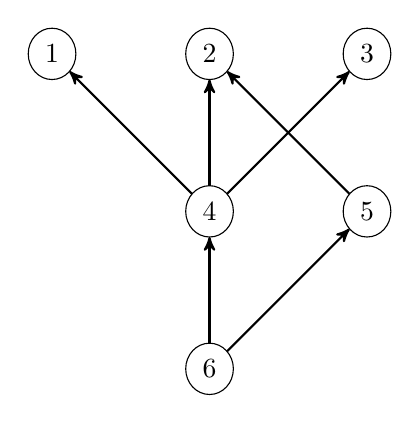
\begin{tikzpicture}[scale=1]
			\tikzstyle{VertexStyle} = [shape = ellipse, minimum width = 4ex, draw]
			\tikzstyle{EdgeStyle}   = [->,>=stealth']
			\SetGraphUnit{2}
			\Vertex{4}
				\NOWE(4){1}
				\NO(4){2}
				\NOEA(4){3}
				\EA(4){5}
				\SO(4){6}
			\Edges(4,1) \Edges(4,2) \Edges(4,3)
			\Edges(5,2)
			\Edges(6,4)
			\Edges(6,5)
		\end{tikzpicture}
	\caption{Directed Acyclic Graph}\label{chapter:dag:concepts:dag-figure}
\end{figure}

As an application generates tasks it can be the case that one group of tasks is dependent upon another group, a third group of tasks is dependent upon a single task, and there may also be many tasks with no dependencies. Strictly speaking, a DAG is a single connected graph, which is not sufficient to represent this scenario. What is necessary, instead, is a data structure that has the ability to contain many locally connected graphs, and individual nodes, something that might be called a multi-DAG. An example of such a DAG is shown in \FigureGeneral \ref{chapter:dag:concepts:multi-dag-figure}. For the purpose of communication ease, the term DAG is used throughout this chapter and the book, with the intention that it means a multi-DAG, or a collection of DAGs.

\begin{figure}
	\centering
		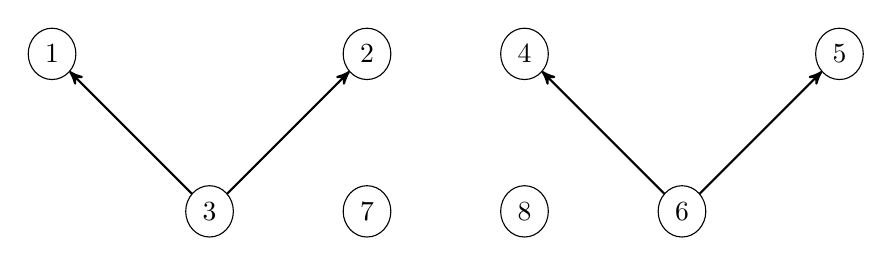
\begin{tikzpicture}[scale=1]
			\tikzstyle{VertexStyle} = [shape = ellipse, minimum width = 4ex, draw]
			\tikzstyle{EdgeStyle}   = [->,>=stealth']
			\SetGraphUnit{2} 
			\Vertex{3}
				\NOWE(3){1}
				\NOEA(3){2}
				\EA(2){4}
				\SOEA(4){6}
				\NOEA(6){5}
				\EA(3){7}
				\WE(6){8}
			\Edges(3,1) \Edges(3,2)
			\Edges(6,4) \Edges(6,5)
		\end{tikzpicture}
	\caption{Multi-DAG}\label{chapter:dag:concepts:multi-dag-figure}
\end{figure}

\subsection{Scheduling Algorithm}\label{chapter:dag:concepts:algorithm}

The DAG is used to represent the task dependencies and an algorithm is needed to traverse the DAG to determine the next available task. The standard first-thought answer to this part of the problem is to use a topological sort\footnote{http://en.wikipedia.org/wiki/Topological\_sorting} to determine the order; given a DAG, a topological sort will provide a valid ordering of the tasks. For any given DAG, there may be multiple correct orderings, any one of which is valid with respect to scheduling. For example, the DAG in \FigureGeneral \ref{chapter:dag:concepts:dag-figure} has a possible ordering of: 1, 2, 3, 4, 5, 6. It also has an alternative, and just as correct, ordering of: 3, 1, 2, 5, 4, 6.

For a single processor system, this is easy enough, simply compute the ordering and feed in that order. However, we are concerned with scalability over a number of processing cores. Therefore, additional insight is necessary to not only build a valid framework mechansim, but also consider application level concerns for task dependencies.

Consider a system with three CPU cores, and also assume equal computational effort for each of the tasks. For \FigureGeneral \ref{chapter:dag:concepts:dag-figure} the ordering of the tasks looks like: (1, 2, 3), (4, 5, x), and (6, x, x). In the first step, all three CPU cores are busy, in the second step, only two of the CPU cores are busy because task 6 has to wait for tasks 4 and 5 to complete. Finally, in the third step, only one CPU core is busy. Again, this is important to understand not only for the framework in how it responds to worker thread requests for something from the work queue, but also for application level design, ensuring there aren't too many dependencies between tasks, resulting in low system utilization.

There is still an additional level of complexity that exists in an operational system. In an interactive (and most others) application, the DAG is dynamic, with tasks coming and going throughout the application lifetime, in addition to tasks having differing levels of computational complexity. For example, going back to the example from \FigureGeneral \ref{chapter:dag:concepts:dag-figure}, let's say that two more tasks, task 7 and 8, show up while tasks 1, 2, and 3 are being computed.  The overall ordering would then look like: (1, 2, 3), (4, 5, 7), and (6, 8, x). Notice that task 7 is computed before task 6, even though it arrived afterwards. A mix of dependent and independent tasks offer the best opportunity for scalability, while also increasing the complexity of the scheduling framework.

The standard topological sorting will correctly handle the ordering of the queue at any time we wish to take a snapshot for a full connected DAG. However, it doesn't handle operational situations with tasks coming and going, some issues with respect to concurrency, or multi-DAGs. What is needed is an algorithm that provides topological-like sorting, but in the context of a dynamic multi-DAG.

The answer to the problem involves two modifications. The first is to keep track of tasks that have been removed from the queue, but have not yet completed execution. This is required to ensure tasks that depend upon removed but not completed tasks are not selected for execution. The second is to take the next available item from the DAG, rather than computing the ordering of all items in the queue. This requires the algorithm check to ensure the task has no dependencies on other tasks awaiting execution, but also that it has no dependencies on tasks that have been removed but have not yet completed execution. The result is still a topological-like sorting, but also correctly manages the additional complexity of an operational context.

\section{Building Blocks}\label{chapter:dag:building-blocks}

This section of the chapter walks through the implementation, highlighting the changes needed to transform the framework code from Chapter \ref{chapter:scalable-task-based} into one that supports task dependencies. The changes to the task scheduling framework are moderate, and involve changing the interface through which tasks are added. The changes to the application are similarly moderate, involving changes to the Mandelbrot tasks, along with changing how the application adds tasks for execution. The updated interactive Mandelbrot viewer is detailed in Section \ref{chapter:dag:app-demo}.

\subsection{Directed Acyclic Graph}\label{chapter:dag:impl:dag}

As with the introduction of priority to the framework, the most interesting part of the changes introduced with this chapter is the implementation of the DAG; noting the implementation is that of the multi-DAG described earlier. There is no ready-made standard library data structure available, instead it is necessary to build a custom data structure. Rather than starting from scratch, and keeping with the theme of this book in taking advantage of the C++ language and framework, a data structure is composed using existing standard library components. Specifically, the \texttt{std::unordered\_map} and \texttt{std::unordered\_set} are used to perform a lot of heavy lifting, which signficantly reduces the amount of custom code. The name of the new data structure is \texttt{ConcurrentDAG}. Like the data structures introduced in the previous two chapters, as its name suggests, it is thread-safe. The remainder of this section details the implementation.

\subsubsection{Task Identification \& Ordering}

With the ability to define dependencies between tasks, some way is needed to uniquely identify a task. Additionally, the scheduling system needs to have a way of knowing the time-based ordering of tasks. In order to achieve this, I have chosen to add an \texttt{uint32\_t} identifier to the \texttt{Task} class. The revised \texttt{Task} declaration and constructor implementation are found in \FigureCode \ref{chapter:dag:impl:task}.

\begin{code}[caption={Revised \texttt{Task} Class}, label=chapter:dag:impl:task]
class Task
{
public:
  explicit Task(std::function<void()> onComplete);
  virtual ~Task()  {}

  uint32_t getId() const { return m_id; }
  virtual void execute() = 0;
  void complete()        { if (m_onComplete) { m_onComplete(); } }

protected:
  uint32_t m_id;

private:
  std::function<void ()> m_onComplete;
};

Task::Task(std::function<void ()> onComplete) :
  m_onComplete(onComplete)
{
  static uint32_t currentId = 1;
  static std::mutex myMutex;

  std::lock_guard<std::mutex> lock(myMutex);

  m_id = currentId++;

  if (currentId == std::numeric_limits<uint32_t>::max())
  {
    currentId = 1;
  }
}
\end{code}

The key part of this class is the technique used to assign the unique id. A \texttt{static} \texttt{currentId} is intially assigned a value of \texttt{1}. The first \texttt{Task} instance is assigned this value, then the \texttt{currentId} is incremented. This serves two purposes. The first is that each task is assigned a unique identifier. Secondly, because of the linearly increasing values, an implicit time-based ordering of the tasks is provided. Notice that a \texttt{std::mutex} is used to protect the assignment and update of the \texttt{currentId}; this ensures the code is thread-safe, meaning that mutliple threads can safely create instances of this class and expect that unique ids are generated.

Even though the \texttt{ConcurrentDAG} class is written as a template type, for the purposes of this book, the type is only ever expected to be a \texttt{std::shared\_pointer<Task>}. Specifically the \texttt{ConcurrentDAG} expects the template type \texttt{T} to have a \texttt{getId()} method. This method is expected to return a unique identifier for each instance stored in the data structure.

\subsubsection{Data Members}

Several pieces of data have to be tracked in order to construct the DAG functionality. The declaration for these data members is found in \FigureCode \ref{chapter:dag:impl:data-members}. The first, \texttt{m\_nodes}, is a set of all tasks either waiting for execution or in execution but pending completion. The \texttt{m\_nodes} member is a \texttt{std::map} in order to return items in sorted (i.e. time-based) order as they are dequeued; all other \texttt{map}s are \texttt{std::unordered\_map}s for best possible performance. Next, \texttt{m\_inUse}, is the set of tasks that have been selected for execution, but have not yet completed; the tasks in this container are still references in the \texttt{m\_nodes} container. A task may have other tasks depending upon it for completion before they can execute. A container for tracking these dependencies is needed; this is sometimes known as an adjacency list. These dependencies are identified in the \texttt{m\_adjacent} container. Finally, when looking for the next task available for computation another container, \texttt{m\_reference}, is needed to help speed up the search for tasks that have no references in the \texttt{m\_adjacent} container. How these data structures are used is highlighted as the class methods are discussed later in the chapter.

\begin{code}[caption={\texttt{ConcurrentDAG} Data Members}, label=chapter:dag:impl:data-members]
std::map<uint32_t, Node> m_nodes;
std::unordered_set<uint32_t> m_inUse;
std::unordered_map<uint32_t, std::unordered_set<uint32_t>> m_adjacent;
std::unordered_map<uint32_t, std::unordered_set<uint32_t>> m_reference;
\end{code}

\subsubsection{Adding Tasks}

There are two contexts in which tasks are added to the DAG. The first is adding a task that has no dependencies, the second is adding a group of tasks that have dependencies within that group. Although it is easily argued that adding a single task is a subset of adding a group, in practice it turns out to be better to write code to handle these cases independently. Another important consideration is that adding a group of tasks with dependencies must be handled as an atomic operation; no other tasks can be added or removed while the group is added. 

Because of the need to ensure all tasks in a group are added atomically, the concept of a group operation is included as part of the \texttt{ConcurrentDAG}. This is provided through two simple methods that must be used to wrap the adding of the tasks. The names of these methods are \texttt{beginGroup} and \texttt{endGroup}, their implemention is shown in \FigureCode \ref{chapter:dag:impl:group}.

\begin{code}[caption={Group Operations}, label=chapter:dag:impl:group]
void beginGroup()    { m_mutex.lock(); }
void endGroup()      { m_mutex.unlock(); }
\end{code}

The implementation for these methods is trivial, but important. They obtain a lock on a mutex; noting all other operations on the \texttt{ConcurrentDAG} require obtaining a lock on this mutex. The type of mutex used is a \texttt{std::recursive\_mutex}. This type of mutex allows a thread that has already obtained a lock on a mutex to pass through when it tries to obtain it again. In other words, a thread can call \texttt{beginGroup}, which obtains the mutex lock, then make another call that requires the mutex lock and pass right through, while other threads are blocked on the same methods. The use of the mutex not only ensures thread safety, it also ensures the thread that obtained the lock is the only one able to add new tasks.

Therefore, when adding a group of related tasks, the \texttt{beginGroup} method is called first, the tasks are added, then \texttt{endGroup} is called. Between these two calls, tasks are added through the \texttt{addEdge} method. The code for this method is shown in \FigureCode \ref{chapter:dag:impl:add-edge}. The method is named \texttt{addEdge} because it is not only adding tasks to the DAG, but is also adding an edge (a dependency) between the tasks. The \texttt{source} parameter identifies the task that must be executed before the task identified by the \texttt{dependent} parameter.

\begin{code}[caption={Adding Tasks with Dependencies}, label=chapter:dag:impl:add-edge]
void addEdge(T source, T dependent)
{
  std::lock_guard<std::recursive_mutex> lock(m_mutex);

  m_nodes[source->getId()] = source;
  m_nodes[dependent->getId()] = dependent;

  if (m_adjacent.find(source->getId()) == m_adjacent.end())
  {
    m_adjacent[source->getId()] = std::unordered_set<uint32_t>();
  }
  m_adjacent[source->getId()].insert(dependent->getId());

  if (m_reference.find(dependent->getId()) == m_reference.end())
  {
    m_reference[dependent->getId()] = std::unordered_set<uint32_t>();
  }
  m_reference[dependent->getId()].insert(source->getId());
}
\end{code}

The first step in the method is to grab the recursive mutex. In the case of a group operation, the thread will already own the lock from a call to \texttt{beginGroup} and pass through. Next, both the \texttt{source} and \texttt{dependent} tasks are added to the container that tracks all tasks currently in the DAG. Because \texttt{m\_nodes} is a \texttt{std::map}, if the task is already in the container it isn't duplicated, it simply overwrites itself; this is faster than searching and then adding if it doesn't exist.

The next step in \texttt{addEdge} is to add the \texttt{dependent} task as an \textit{adjacent} task to the \texttt{source}. Adjacent tasks are those that depend upon the \texttt{source} to complete before they can be dequeued for use. Finally, the last step is to add the \texttt{source} task to a \texttt{m\_reference} container. This container allows for quick lookup, when dequeing the next available task, to determine if the candidate task is \textit{referenced} as a dependent to another task. By having each \texttt{dependent} task maintain a set of \texttt{source} tasks upon which it depends, it makes the search trivial, rather than having to look for the task in all other \texttt{source} tasks.

Adding a single task to the DAG is trivial, as compared to adding two. The first difference is that it is not necessary to invoke the \texttt{beginGroup} and \texttt{endGroup} methods. The second, is the code for adding a single node is requires only that the node is added to the master list of tasks and setting its adjaceny list to an empty set. The code for the \texttt{addNode} method is shown in \FigureCode \ref{chapter:dag:impl:add-single}.

\begin{code}[caption={Adding a Single Task}, label=chapter:dag:impl:add-single]
void addNode(T one)
{
  std::lock_guard<std::recursive_mutex> lock(m_mutex);

  m_nodes[one->getId()] = one;
  m_adjacent[one->getId()] = std::unordered_set<uint32_t>();
}
\end{code}

\subsubsection{Dequeueing \& Removing Tasks}

A task goes through a two-step dequeue and removal process before it is completely eliminated from the DAG. The first step is to dequeue the task for execution. At this point, the task is identified as \textit{in use} (i.e., being executed), but still considered part of the DAG so as to prevent dependent tasks from being dequeued for execution. The second step is the final removal of the task from the DAG upon completion. In this step the task is fully removed from the DAG, allowing dependent tasks to be dequeued.

The code for dequeuing a task from the DAG is shown in \FigureCode \ref{chapter:dag:impl:dequeue}. As with all other methods, the first step in \texttt{dequeue} is to grab a lock on the mutex. Once the lock is obtained, the list of all tasks is searched for a task that is not dependent upon any other tasks or any tasks currently in use. The search of all tasks isn't a random search, it is in order by the oldest tasks. This happens by design through the use of a \texttt{std::map}, which is a binary search tree (\texttt{std::unordered\_map} is an unordered hash table). The ordering of the tasks in \texttt{m\_nodes} is based upon the \texttt{Task::m\_id} member, which is an \texttt{uint32\_t} that is assigned an increasing value based upon when it was created.

\begin{code}[caption={Dequeing a Task}, label=chapter:dag:impl:dequeue]
T dequeue()
{
  std::lock_guard<std::recursive_mutex> lock(m_mutex);

  T item = nullptr;
  bool found = false;
  for (const auto& candidate : m_nodes)
  {
    auto itr = m_reference.find(candidate.first);
    if ((itr == m_reference.end() ||
      itr->second.size() == 0) &&
      m_inUse.find(candidate.first) == m_inUse.end())
    {
      found = true;
      item = candidate.second;
      m_inUse.insert(candidate.first);
      break;
    }
  }

  return item;
}
\end{code}

It is easy to determine if a task is dependent upon another task by checking the \texttt{m\_reference} data structure. If the task is not found in the data structure, or is found but has a size of 0, then it isn't reliant upon a task not yet dequeued. However, it may still be dependent upon an in use task. This is also easily determined by looking for a reference to it in the \texttt{m\_inUse} set. If the \texttt{candidate} task is found to not be dependent upon any other tasks, it is assigned to the local \texttt{item} variable, added to the \texttt{m\_inUse} set, \texttt{found} set to \texttt{true}, and the search loop ended. Because the \texttt{Task} information is no longer needed, only the \texttt{Task::m\_id} (stored as the key in the \texttt{candidate.first} member) is stored in the \texttt{m\_inUse} set. In the case no task is found that meets the criteria, or none exist at all, the \texttt{item} variable remains set to the \texttt{nullptr} and the method returns.

When a task has completed execution, its needs to be completely removed from the DAG. The method for doing this is called \texttt{finalize} and is show in \FigureCode \ref{chapter:dag:impl:finalize}. This method first performs a quick check to see if the task being finalized actually exists in the \texttt{m\_inUse} set. This is only done as an \texttt{assert} so that program logic errors can be discovered, release builds will not have this check. Next, the code goes through all of its adjacent tasks and removes references to itself from those tasks. This removes the dependency from this task to any other task in the DAG. The code then cleans up the \texttt{m\_adjacent} set by erasing it. Finally, the task itself is removed from both the master set of tasks and the in use tasks. When this method exits, the task is no longer a part of the DAG, and any tasks previously dependent upon its completion are now free to be dequeued.

\begin{code}[caption={Finalizing a Task}, label=chapter:dag:impl:finalize]
void finalize(const T& node)
{
  std::lock_guard<std::recursive_mutex> lock(m_mutex);

  assert(m_inUse.find(node->getId()) != m_inUse.end());

  for (auto id : m_adjacent[node->getId()])
  {
    m_reference[id].erase(node->getId());
  }
  m_adjacent.erase(node->getId());
  m_nodes.erase(node->getId());
  m_inUse.erase(node->getId());
}
\end{code}

\subsection{Thread Pool}

The public interface to the \texttt{ThreadPool} is changed from both the previous chapters. The changes to the interface are made to support the ability to add tasks that depend upon other tasks. The interface exposed by the \texttt{ThreadPool} matches that of the \texttt{ConcurrentDAG} as detailed in Section \ref{chapter:dag:impl:dag}. \FigureCode \ref{chapter:dag:thread-pool:declaration} shows the revised \texttt{ThreadPool} class declaration.

\begin{code}[caption={\texttt{ThreadPool} Declaration}, label=chapter:dag:thread-pool:declaration]
class ThreadPool
{
public:
  static std::shared_ptr<ThreadPool> instance();
  static void terminate();

  void beginGroup()    { m_taskDAG.beginGroup(); }
  void endGroup()      { m_taskDAG.endGroup(); }
  void enqueueTask(std::shared_ptr<Task> source);
  void enqueueTask(
    std::shared_ptr<Task> source, 
    std::shared_ptr<Task> dependent);

protected:
  ThreadPool(uint16_t sizeInitial);

private:
  static std::shared_ptr<ThreadPool> m_instance;
  friend WorkerThread;

  std::vector<std::shared_ptr<WorkerThread>> m_threadQueue;
  ConcurrentDAG<std::shared_ptr<Task>> m_taskDAG;
  std::condition_variable m_eventDAG;

  void taskComplete();
};
\end{code}

The application interface to the \texttt{ThreadPool} is nearly identical to the \texttt{ConcurrentDAG}, because it is essentially a pass-through wrapper around the \texttt{ConcurrentDAG}. The \texttt{beginGroup} and \texttt{endGroup} methods simply invoke the underlying \texttt{m\_taskDAG} methods. The two \texttt{enqueueTask} methods invoke the \texttt{addNode} and \texttt{addEdge} methods of the \texttt{m\_taskDAG}. Additionally, these \texttt{enqueueTask} methods signal the \texttt{m\_eventDAG} to ensure a worker thread is released so the task can potentially be dequeued from the DAG. The code for these two methods is found in \FigureCode \ref{chapter:dag:thread-pool:enqueue-task}.

\begin{code}[caption={\texttt{ThreadPool::enqueueTask} Methods}, label=chapter:dag:thread-pool:enqueue-task]
void ThreadPool::enqueueTask(std::shared_ptr<Task> source)
{
  m_taskDAG.addNode(source);
  m_eventDAG.notify_one();
}

void ThreadPool::enqueueTask(
  std::shared_ptr<Task> source, 
  std::shared_ptr<Task> dependent)
{
  m_taskDAG.addEdge(source, dependent);
  m_eventDAG.notify_one();
}
\end{code}

The one new structural addition to the \texttt{ThreadPool} is the \texttt{taskComplete} method. The implementation of this method is found in \FigureCode \ref{chapter:dag:thread-pool:task-complete}. The purpose of this method is to allow \texttt{WorkerThread}s to inform the \texttt{ThreadPool} when a task has completed execution. On completion of a task, more than one dependent task may become available for computation. Therefore, multiple worker threads must be signaled to that any available tasks are grabbed for computation.

\begin{code}[caption={\texttt{ThreadPool::taskComplete} Method}, label=chapter:dag:thread-pool:task-complete]
void ThreadPool::taskComplete() 
{
  m_eventQueue.notify_all(); 
}
\end{code}

\subsection{Worker Thread}\label{chapter:dag:impl:worker-thread}

Worker threads continue to have the same fundamental purpose, as used in Chapter \ref{chapter:scalable-task-based}, watch the task queue and grab the next available task. The change this time is that the tasks come from a DAG, which may describe complex inter-relationships between the tasks, which affect the order in which they are removed.

The revised constructor is shown in \FigureCode \ref{chapter:dag:worker-thread:constructor}. The constructor returns to looking much like the \texttt{WorkerThread} from Chapter \ref{chapter:scalable-task-based}. The constructor accepts parameters that provide references to the \texttt{ConcurrentDAG} which contains the tasks, along with the \texttt{std::condition\_variable} used to signal when tasks are added to the DAG. The body of the constructor creates the thread associated with the worker.

\begin{code}[caption={\texttt{WorkerThread} Constructor}, label=chapter:dag:worker-thread:constructor]
WorkerThread::WorkerThread(
    ConcurrentDAG<std::shared_ptr<Task>>& taskDAG, 
    std::condition_variable& taskDAGEvent) :
  m_taskDAG(taskDAG),
  m_eventTaskDAG(taskDAGEvent),
  m_done(false),
  m_thread(nullptr)
{
  m_thread = std::unique_ptr<std::thread>(
    new std::thread(&WorkerThread::run, this));
}
\end{code}

The \texttt{run} method has changed somewhat to support the way tasks are represented in the DAG. The revised method is shown in \FigureCode \ref{chapter:dag:worker-thread:run}. The only difference in this method versus the one in Chapter \ref{chapter:scalable-task-based} is the addition of two statments. The first is \texttt{m\_taskDAG.finalize(task)}. This statement tells the DAG to remove any reference of the task from the DAG. Remember that DAG-based tasks have a two-step use case: they are first dequeued, then finalized. The other additional statement is \texttt{ThreadPool::instance()->taskComplete()}. This statement informs the \texttt{ThreadPool} a task has just finished execution, causing it to signal all worker threads so that all dependent tasks possibly released are now grabbed and executed.

\begin{code}[caption={\texttt{WorkerThread::run} Method}, label=chapter:dag:worker-thread:run]
void WorkerThread::run()
{
  while (!m_done)
  {
    std::shared_ptr<Task> task = m_taskDAG.dequeue();
    if (task != nullptr)
    {
      task->execute();
      task->complete();
      m_taskDAG.finalize(task);
      ThreadPool::instance()->taskComplete();
    }
    else
    {
      std::unique_lock<std::mutex> lock(m_mutexEventTaskDAG);
      m_eventTaskDAG.wait(lock);
    }
  }
}
\end{code}

\section{Application Task Dependencies}\label{chapter:dag:app-demo}

In addition to revising the framework to include the concept of task dependencies, the interactive Mandelbrot viewing application is also revised to utilize the ability to define task dependencies. This is done by defining a new \texttt{MandelFinishedTask} that is dependent upon the \texttt{MandelPartTask} tasks. The prime number task remains the same, as only one is ever in existence at any time. The \texttt{MandelImageTask} is now removed, with its purpose no longer necessary with the new task depencency framework in place. The other revision to the application code is that tasks are now added using the new \texttt{ThreadPool} interface.

The new \texttt{MandelFinishedTask} class is shown in \FigureCode \ref{chapter:dag:app-demo:mandel-finished-task}. Interestingly, this task doesn't actually do anything, so what is its purpose? The purpose is to act as a kind of signal to the application code that a new Mandelbrot image has completed and it is okay to copy those pixels into the image currently being rendered. The way this works, is to make this task dependent upon all of the \texttt{MandelPartTasks}. When those tasks have all finished, the \texttt{MandelFinishedTask} is removed from the DAG and executed.

\begin{code}[caption={\texttt{MandelFinishedTask}}, label=chapter:dag:app-demo:mandel-finished-task]
class MandelFinishedTask : public Task
{
public:
  MandelFinishedTask(std::function<void ()> onComplete) :
    Task(onComplete)
  {
  }

  virtual void execute() {}
};
\end{code}

Still, the question remains, how does this signal the application, the task doesn't do anything! The answer to the question is in the revised \texttt{Mandelbrot::startNewImage} method, shown in \FigureCode \ref{chapter:dag:app-demo:start-new-image}. The first part of the method creates an instance of a \texttt{MandelFinishedTask}, and this is the key, passes a lambda to the \texttt{onComplete} parameter that copies the newly computed pixels into the image currently being rendered. In other words, while this task performs no computation itself, its \texttt{onComplete} operation is copying the newly computed data into the rendered image.

\begin{code}[caption={\texttt{startNewImage} Method}, label=chapter:dag:app-demo:start-new-image]
void Mandelbrot::startNewImage()
{
  auto taskFinished = std::make_shared<MandelFinishedTask>(
    [this]()
    {
      copyToPixels();
      m_inUpdate = false;
    });

  ThreadPool::instance()->beginGroup();

  double deltaY = (m_mandelBottom - m_mandelTop) / m_sizeY;
  for (auto row : IRange<decltype(m_sizeY)>(0, m_sizeY - 1))
  {
    auto task = std::shared_ptr<MandelPartTask>(
      new MandelPartTask(
        m_image.get() + row * m_sizeX, 
        m_sizeX, MAX_ITERATIONS,
        m_mandelTop + row * deltaY,
        m_mandelLeft, m_mandelRight, 
        nullptr));

    ThreadPool::instance()->enqueueTask(task, taskFinished);
  }

  ThreadPool::instance()->endGroup();
}
\end{code}

The second part of the method, beginning with the \texttt{ThreadPool::instance()->beginGroup()} statement, prepares the tasks that perform the Mandelbrot image computation. The loop goes through each row in the image and creates a \texttt{MandelPartTask} for that row. As the task is added to the \texttt{ThreadPool}, the \texttt{taskFinished} is identified as being dependent upon it. After all of the row tasks are added, a call to \texttt{endGroup} is made, telling the \texttt{ThreadPool} the current group of dependent tasks is complete. With these task dependencies set up, the scheduling framework takes over and ensures all of the \texttt{MandelPartTask}s are complete, before the \texttt{MandelFinishedTask} is executed.

% consider showing profiling results from the Scalable and DAG applications that show there is no longer a thread sitting around doing nothing.

\subsection{Further Demonstration}\label{chapter:dag:app-demo:non-trivial}

The demonstration application provided as part of this chapter includes an additional task and application code that provides a better run-time demonstration of the use of task dependencies. A new task named \texttt{SimpleTask} is added that waits for a specified amount of time. A new function named \texttt{startChapterDemo} is added that creates a non-trivial set of task dependencies that match those found in \FigureGeneral \ref{chapter:dag:concepts:dag-figure}.

The code for the new task is found in \FigureCode \ref{chapter:dag:app-demo:simple-task}. The task accepts an \texttt{uint16\_t}, used to identify the task for display. When the task is executed it goes to sleep for 3000 milliseconds, then shows its name. The only purpose of this task is to aid in demonstrating the order in which tasks are executed.

\begin{code}[caption={\texttt{SimpleTask}}, label=chapter:dag:app-demo:simple-task]
class SimpleTask : public Task
{
public:
  SimpleTask(uint16_t name) :
    Task(nullptr),
    m_name(name)
  {}

  virtual void execute() 
  {
    std::this_thread::sleep_for(std::chrono::milliseconds(3000));
    std::cout << m_name << std::endl;
  }

private:
  uint16_t m_name;
};
\end{code}

The code for the new \texttt{startChapterDemo} is found in \FigureCode \ref{chapter:dag:app-demo:chapter-demo}. This method creates a set of \texttt{SimpleTask}s that match those found in \FigureGeneral \ref{chapter:dag:app-demo:simple-task}. The first part of the method creates the tasks and identifies them by their number. Finally, the method adds the tasks to the \texttt{ThreadPool}, defining the various dependencies among the tasks. Task 2 is referenced twice in order to define the relationship between it and tasks 4 and 5. Also, tasks 4 and 6 are referenced multiple times in order to define their dependencies upon more than one parent tasks. Remember that even though a task is referenced more than once doesn't mean it is computed multiple times, the \texttt{ConcurrentDAG} ensures a task is added only once, regardless of the number of times it is referenced.

\begin{code}[caption={\texttt{startChapterDemo} Method}, label=chapter:dag:app-demo:chapter-demo]
void ScalabilityApp::startChapterDemo()
{
  ThreadPool::instance()->beginGroup();

  auto task1 = std::make_shared<SimpleTask>(1);
  auto task2 = std::make_shared<SimpleTask>(2);
  auto task3 = std::make_shared<SimpleTask>(3);
  auto task4 = std::make_shared<SimpleTask>(4);
  auto task5 = std::make_shared<SimpleTask>(5);
  auto task6 = std::make_shared<SimpleTask>(6);

  ThreadPool::instance()->enqueueTask(task1, task4);
  ThreadPool::instance()->enqueueTask(task2, task4);
  ThreadPool::instance()->enqueueTask(task2, task5);
  ThreadPool::instance()->enqueueTask(task3, task4);
  ThreadPool::instance()->enqueueTask(task4, task6);
  ThreadPool::instance()->enqueueTask(task5, task6);

  ThreadPool::instance()->endGroup();
}
\end{code}

When the program is run, the first three tasks, 1, 2, and 3 are executed in parallel (if enough CPU cores). Once task 2 has completed, task 5 becomes available and begins computation. When all three of tasks 1, 2, and 3 complete, task 4 is released and begins computation. Finally, when tasks 4 and 5 complete, task 6 is released and begins computation. On my computer, tasks 1, 2, and 3 all compute in parallel, when they are finished, 4 and 5 compute in parallel, and finally task 6 executes. This code shows how a non-trivial set of relationships between tasks is easily expressed in application code, and the hard work of scheduling the tasks is left to the underlying scheduling framework.

\section{Summary}\label{chapter:dag:summary}

This chapter introduced the concept of allowing dependencies between tasks through the use of a DAG-based scheduling framework. This provides an extremely powerful tool for an application developer through simplified application code by placing the algorithmic complexity in the scheduling framework. To achieve this, the underlying framework required a number of changes, most noteworthy of which is the introduction of a DAG-based data structure used for determing the order in which tasks can be removed for computation. Having this new capability simplified the application code, while also making better use of the thread pool framework.

	% Copyright � 2015 by James Dean Mathias
% All Rights Reserved

\chapter{Networking Techniques}\label{chapter:networking}

This chapter discusses the networking techniques used for the distributed applications presented in the next chapters. The foundation for the network communication comes from the Boost (\href{http://www.boost.org}{http://www.boost.org}) libraries, introduced in Section \ref{chapter:networking:boost:introduction}. The Boost libraries are used in combination with the new C++11 threading and lambda features to form clean solutions for the networking code.

The choice to use Boost is driven by its cross-platform approach, the well designed interfaces, along with its developer friendly license. A testament to its design and utility is the large number of libraries that have made it into the C++11, and C++14, standards. In particular, the networking API (Boost.Asio) is well designed, easy to use, and works well across a number of different compiler and OS platforms.

The networking techniques presented in this chapter and used by the demonstration applications detailed in this book have worked well for my research and work. This chapter is not a comprehensive discussion of Boost.Asio, only those techniques directly applied throughout the rest of the book are discussed. There are any number of designs and philisophies that may be taken, owing to the needs of the application being developed and to personal preferences. Consider the networking technique used in this book as a recommendation, but not necessarily one that fits the needs for every application and developer.

\section{Boost Introduction}\label{chapter:networking:boost:introduction}

Boost is a set of cross-platform C++ libraries that provide a broad range of capabilties. In fact, many of these capabilities have found their way into C++11 language and standard libraries, including smart pointers, threading, and lambda functions. Of primary interest for this book is the low-level networking API Boost.Asio, or simply Asio. Goals for the Boost.Asio library include \textit{Portability}, \textit{Scalability}, \textit{Efficiency}, and \textit{Ease of use}. Boost.Asio provides an asynchronous I/O abstraction for things like serial ports, file descriptors, and networking. The focus in this chapter, and the book, is on its use for networking.

The Boost set of libaries is friendly for use by both commercial and non-commercial organizations, provided for by its own license, the Boost Software License\footnote{http://www.boost.org/LICENSE\_1\_0.txt}. The license is BSD like, certified \textit{Open Source} by the Open Source Initiative, comes \textit{as is}, allows for the use and modification of the Boost libraries, does not require the license is distributed with binary or executable uses of the libraries, along with not requiring the source is made available external to the organization.

The Boost libaries are updated several times a year to include new capabilities, improve efficiency, and resolve outstanding bugs; at the time of this writing the current version is 1.57. A large number of the commonly used libraries are mature and stable, and care is taken to maintain backwards compatibility. Additionally, the library is verified against a large number of C++ compilers and operating system platforms. This gives developers confidence their code won't break with each new library update.

\section{Boost Asio}\label{chapter:networking:asio}

Boost.Asio is the library upon which networking I/O operations are built. It supports both synchronous and asynchronous operations in single and multi threaded applications. In addition to networking operations, other capabilities are exposed, such as timers, signal handling, and even SSL operations. The focus in this chapter, and the book, is on the networking operations.

The Boost.Asio library provides a model of its own that must be understood to take full advantage of its capabilities; it is not simply a thin wrapper around the \textit{sockets} API. This chapter provides a solid introduction to the library and the way in which I have found to work well for my application development style, but it is strongly recommended to refer to the Boost.Asio online documentation\footnote{http://www.boost.org/doc/libs/1\_57\_0/doc/html/boost\_asio.html} for a complete description of its design, rationale, and use.

\subsection{Asio io\_service}\label{chapter:networking:asio:ioservice}

The foundation for Boost.Asio operations is the \texttt{io\_service}. Understanding its role and operation is essential for developing correct and efficient networking applications. Every application must instantiate an \texttt{io\_service} through which all operations are managed. The \texttt{io\_service} maintains a queue of operations that it needs to service. The operations on this queue are only serviced by the thread (or threads) that call its \texttt{.run} method. The \texttt{.run} method blocks until all these operations have completed. Using the C++11 lambda and threading features, it is trivial to create a worker thread that is dedicated to the \texttt{io\_service} queue, leaving the main application thread free to work on other tasks. The code in \FigureCode \ref{chapter:networking:ioservice-thread} illustrates how this may be done.

\begin{code}[caption={io\_service Thread}, label=chapter:networking:ioservice-thread]
boost::asio::io_service ioService;
std::thread ioThread = std::thread(
  [&ioService]()
  {
    ioService.run();
  });
\end{code}

The first statement instantiates the \texttt{io\_service}, causing it to come to life. The next statment invokes a thread, using a lambda to define the thread function, and calls the \texttt{.run} method of the \texttt{io\_service}. This code will correctly create an \texttt{io\_service} and create a thread to service any queued operations. Note that the \texttt{.run} method will fall through (unblock) when there are no more queued operations. Therefore, this code will immediately fall through, closing down the \texttt{io\_service} thread, which is something we do not want.

The solution to the above problem is to create an \texttt{io\_service::work} object which prevents the \texttt{.run} method from unblocking until the \texttt{io\_service} is stopped. The purpose of this object is to inform the \texttt{io\_service} it has work remaining to do, preventing it from falling through the \texttt{.run} method until \texttt{.stop} is called on the \texttt{io\_service}. The code in \FigureCode \ref{chapter:networking:ioservice-work} demonstrates the use of the \texttt{io\_service::work} object.

\begin{code}[caption={io\_service::work Object}, label=chapter:networking:ioservice-work]
boost::asio::io_service ioService;
boost::asio::io_service::work work(ioService);

std::thread ioThread = std::thread(
  [&ioService]()
  {
    ioService.run();
    std::cout << "Completed ioService." << std::endl;
  });

std::cout << "Sleeping for a couple of seconds..." << std::endl;
std::this_thread::sleep_for(std::chrono::milliseconds(2000));
std::cout << "Stopping the ioService..." << std::endl;

ioService.stop();
ioThread.join();
\end{code}

In this code an \texttt{io\_service::work} object is created and initialized with a reference to the \texttt{ioService} instance. Inside the thread function (a lambda) the \texttt{ioService.run();} statement blocks until the \texttt{ioService.stop();} statement in the main thread is executed. A sleep operation is executed to demonstrate that the thread does not complete until the \texttt{ioService} object is told to stop. Following the \texttt{ioService.stop();} statement the \texttt{ioService} thread is joined and then the code is allowed to continue.

Using this approach, a separate worker thread is created and used to service all operations placed on the \texttt{io\_service} queue, with the worker thread staying active until the \texttt{io\_service} is specifically stopped. The next section, Section \ref{chapter:networking:asio:ioservice:queue} discusses how to place operations on the queue.

\subsection{The \texttt{io\_service} Queue}\label{chapter:networking:asio:ioservice:queue}

The \texttt{io\_service} object maintains a queue onto which requests are placed and from which they are serviced; it is a first in, first out (FIFO) queue. Requests get placed on this queue implicitly through the use of some of the Boost.Asio API calls, while others are explicitly placed on the queue through the use of the \texttt{.post} method. Most of the code presented in this book explicitly places requests using \texttt{.post}, therefore, the focus in this chapter is on its use and behavior.

The code in \FigureCode \ref{chapter:networking:ioservice:post-simple} shows how to post a request to an \texttt{io\_service} queue. The \texttt{.post} method expects a \texttt{CompletionHandler}, which is function whose signature accepts no parameters and has a \texttt{void} return. In this example, the function is provided by defining a lambda.

\begin{code}[caption={Posting a Request}, label=chapter:networking:ioservice:post-simple]
ioService.post(
  []()
  {
    std::cout << "This runs on the io_service thread.";
  });
\end{code}

The main application thread, or really any application thread, can post to the \texttt{io\_service} queue, such as the one in \FigureCode \ref{chapter:networking:ioservice:post-simple}. Once the \texttt{io\_service} thread works its way through the items ahead of our request, it will invoke the \texttt{CompletionHandler}. In this example, \texttt{This runs on the io\_service thread.} is output to the console.

\FigureCode \ref{chapter:networking:ioservice:post-multiple} shows a full example of defining a dedicated thread for an \texttt{io\_service}, along with posting several requests to its queue. This example starts by reporting the thread ids for the main application thread and the \texttt{io\_service} thread to help establish which threads are executing which code. Each lambda posted to the \texttt{io\_service} reports the thread from which it is executed, in both cases they report the same thread id as the \texttt{io\_service} reported.

\begin{code}[caption={Multiple Requests}, label=chapter:networking:ioservice:post-multiple]
void ioServiceQueue()
{
  boost::asio::io_service ioService;
  boost::asio::io_service::work work(ioService);

  std::cout << "main thread id: ";
  std::cout << std::this_thread::get_id() << std::endl;

  std::thread ioThread = std::thread(
    [&ioService]()
    {
      std::cout << "io_service thread id: ";
      std::cout << std::this_thread::get_id() << std::endl;
      ioService.run();
      std::cout << "io_service terminated" << std::endl;
    });

  auto notify =
    []()
    {
      std::cout << "This post executed on: ";
      std::cout << std::this_thread::get_id() << std::endl;
    };

  ioService.post(notify);
  ioService.post(notify);

  ioService.stop();
  ioThread.join();
}
\end{code}

The Boost.Asio \texttt{io\_service} queue is fairly easy to understand when seen in action like this. Unfortunately, this is about as simple as it gets, most non-trivial applications that utilize network communication require a more sophisticated usage. The next two sections, Section \ref{chapter:networking:threading} and Section \ref{chapter:networking:strands} provide additional stepping stones to building the necessary understanding.

\section{Boost Asio Thread Pools}\label{chapter:networking:threading}

To develop a truly scalable application, we'll need more than a single background thread servicing requests on an \texttt{io\_service} queue. By definition, a \textit{scalable} application should grow to utilize the available system resources. In the case of the system I'm using to develop the code samples for this book, it has 6 hyper-threaded CPU cores, giving the appearance of 12 CPU cores. A scalable application will take advantage of all the cores on my system, and all of the cores on any other system on which it is run. Thankfully, Boost.Asio provides easy support for \textit{Thread Pools} on the \texttt{io\_service}.

In order to have more than one thread service requests from the \texttt{io\_service} queue, simply create more threads that call the \texttt{io\_service} \texttt{.run} method. \FigureCode \ref{chapter:networking:ioservice:thread-pool} shows an example of creating a thread pool on a single \texttt{io\_service}. Through the use of this technique, multiple requests can be serviced in parallel on a multi-core system.

\begin{code}[caption={\texttt{io\_service} Thread Pool}, label=chapter:networking:ioservice:thread-pool]
void threadedIoService()
{
  boost::asio::io_service ioService;
  boost::asio::io_service::work work(ioService);

  std::cout << "main thread id: ";
  std::cout << std::this_thread::get_id() << std::endl;

  std::vector<std::thread> threads;
  for (auto thread : IRange<uint8_t>(1, std::thread::hardware_concurrency()))
  {
    threads.push_back(std::thread(
      [&ioService]()
      {
        ioService.run();
      }));
  }

  auto notify =
    []()
    {
      std::cout << "This post executed on: ";
      std::cout << std::this_thread::get_id() << std::endl;
    };

  ioService.post(notify);
  ioService.post(notify);

  ioService.stop();
  for (auto& thread : threads)
  {
    thread.join();
  }
}
\end{code}

\section{Boost Asio Strands}\label{chapter:networking:strands}

Often times it is necessary to queue the requests for a single object to ensure they happen sequentially, while still allowing requests on other objects to be performed in parallel. Consider that the send operations on a socket can not be interleaved, one must complete before the next is started. We'd like to write code that makes non-blocking write requests, but also ensure that the requests are performed in order and that each request is completed before the next one is allowed to begin. In the normal free-for-all world of thread pools and the \texttt{io\_service} object, that isn't guaranteed. Another synchronization capability is needed, one that allows requests on one object to be queued and completed in order while still participating in the context of a thread pool. That capability is provided by \texttt{io\_service::strand}, Boost strands.

A strand can be thought of as an independent synchronization queue within an \texttt{io\_service}. Each \texttt{io\_service::strand} has its own request queue to which service requests are posted. Even though a strand has its own request queue, it is still associated with an \texttt{io\_service}, passed in as a parameter to the strand constructor. Posts are made directly to the strand, rather than to the \texttt{io\_service}. The \texttt{io\_service::strand} ensures that all post requests to a strand will \textit{not} execute concurrently, instead requests are serviced in the order they are posted and each request is completed before the next is started. Note that requests on multiple strands may execute concurrently, it is only requests on each individual strand are executed sequentially.

Strands are illustrated through a \texttt{Countdown} class that is updated within a thread pool, using an \texttt{io\_service::strand} to guarantee the updates are correctly synchronized. All the \texttt{Countdown} class does is post a bunch of requests to its own strand, with the requests updating an internal counter and reporting the value until the count reaches 0. The full \texttt{Countdown} class is shown in \FigureCode \ref{chapter:networking:strand:countdown-class}.

\begin{code}[caption={\texttt{Countdown} Class}, label=chapter:networking:strand:countdown-class]
class Countdown
{
public:
  Countdown(boost::asio::io_service& ioService, 
      std::string name, 
      uint16_t startCount) :
    m_strand(ioService),
    m_name(name),
    m_count(startCount)
  { }

  void start()
  {
    for (auto handler = 0; handler < m_count; handler++)
    {
      m_strand.post([&]() { next(); });
    }
  }

private:
  boost::asio::strand m_strand;
  std::string m_name;
  uint16_t m_count;

  void next()
  {
      std::cout << "Thread id: ";
      std::cout << std::this_thread::get_id();
      std::cout << " Name: " << m_name;
      std::cout << " - Count: " << m_count << std::endl;
      m_count--;
  }
};
\end{code}

This class defines a private \texttt{strand}, which is associated with the \texttt{io\_service} in the class constructor. It also contains a \texttt{name}, used to identify the instance in console output, and a \texttt{count}, used to track how much longer to continue the countdown. The public method \texttt{start} is called by an application thread to kick off the countdown and reporting for the instance. When invoked, the \texttt{start} method posts \texttt{m\_count} handlers (lambdas) to the object's \texttt{strand}, rather than to an \texttt{io\_service}. As each request is invoked by a thread in the thread pool on the \texttt{io\_service}, the handler reports which thread it is executing on, along with reporting the instance name, and the current value of the counter. The final statement in the hanlder is to subtract one from the value of \texttt{m\_count}.

The application code that demonstrates the use of the \texttt{Countdown} class is found in \FigureCode \ref{chapter:networking:strand:countdown-app}.

\begin{code}[caption={\texttt{Countdown} Application}, label=chapter:networking:strand:countdown-app]
int main()
{
  boost::asio::io_service ioService;
  boost::asio::io_service::work work(ioService);

  std::vector<std::thread> threads;
  for (auto thread : IRange<uint8_t>(1, std::thread::hardware_concurrency()))
  {
    threads.push_back(std::thread(
      [&ioService]()
      {
        ioService.run();
      }));
  }

  Countdown obj1(ioService, "One", 10);
  Countdown obj2(ioService, "Two", 12);

  obj1.start();
  obj2.start();

  for (auto& thread : threads)
  {
    thread.join();
  }

  return 0;
}
\end{code}

The first part of the code is familiar by now, the definition of an \texttt{io\_service} along with a thread pool to service requests. This is followed by two instances of the \texttt{Countdown} class being created and started. Sample output from a run of this program is shown in \FigureConsole \ref{chapter:networking:strand:countdown-output}. I've modified the output a little bit to clean up an issue from multiptle threads writing to the console (which is not synchronized) concurrently, but only for readability, the meaning is not changed.

\begin{console}[caption={\texttt{Countdown} Output}, label=chapter:networking:strand:countdown-output]
Thread id: 7788 Name: One - Count: 10
Thread id: 6652 Name: Two - Count: 12
Thread id: 11252 Name: One - Count: 9
Thread id: 7788 Name: One - Count: 8
Thread id: 11252 Name: Two - Count: 11
Thread id: 6652 Name: One - Count: 7
Thread id: 7788 Name: Two - Count: 10
Thread id: 11252 Name: One - Count: 6
Thread id: 6652 Name: Two - Count: 9
Thread id: 7788 Name: One - Count: 5
Thread id: 11252 Name: Two - Count: 8
Thread id: 6652 Name: One - Count: 4
Thread id: 7788 Name: Two - Count: 7
Thread id: 11252 Name: One - Count: 3
Thread id: 6652 Name: Two - Count: 6
Thread id: 7788 Name: One - Count: 2
Thread id: 11252 Name: Two - Count: 5
Thread id: 6652 Name: One - Count: 1
Thread id: 7788 Name: Two - Count: 4
Thread id: 11252 Name: Two - Count: 3
Thread id: 7788 Name: Two - Count: 2
Thread id: 11252 Name: Two - Count: 1
\end{console}

A careful read through the output shows that each \texttt{Countdown} instance correctly (in-order) performs the countdown as intended. Note also that different thread ids are reported being used on the same \texttt{Countdown} instances. In fact, three different threads were used by the system to service the different requests.

The \texttt{io\_service} and \texttt{strand}s are a part of the Boost.Asio library, and are intended for use in synchronizing I/O operations, but as this code demonstrates, they can be used as a general synchronization resource. To clarify, this code uses the \texttt{io\_service} as a thread pool, then uses \texttt{strand}s as a synchronization object. No where in this code is a mutex defined and used for synchronization, that is taken care of by the Boost.Asio implementation.

\section{Boost Asio Socket Connections}\label{chapter:networking:sockets}

Sockets in Boost.Asio are familiar to anyone already experienced in regular sockets programming, only a little easier to use because of the simplied syntax and elimination of platform initialization dependencies. The sockets API in Boost.Asio provides for both synchronous and asynchronous programming models. The code presented in this chapter, and throughout the book, relies primarily on asynchronous techniques, with a few synchronous pieces where scalability is not an issue.

There are two fundamental components needed to understand socket programming in Boost.Asio. The first is how to make and receive a connection, the second is how to send and receive data. For the purposes of this section, a \textit{server} is the application that receives a connection, and a \textit{client} is the application that initiates a connection. The words \textit{server} and \textit{client} are only ways to refer to different application components. They are used in one way in this chapter, and differently in later parts of this book. Section \ref{chapter:networking:sockets:connection} discusses making connections, and Section \ref{chapter:networking:sockets:data:intro} discusses sending and receiving of data.

Take note that all the techniques described in this chapter, and throughout the book, utilize TCP communication. Many of the programming concepts and techniques are similar between TCP and UDP. While knowing the TCP programming model is helpful to understanding similar looking UDP API, UDP application development is a different model, one not covered in this book.

\subsection{Boost \texttt{endpoint} and IPv4 \& IPv6}

Before getting into the details of making connections and sending data, it is important to discuss the Boost \texttt{endpoint} type. An \texttt{endpoint} describes an endpoint that can be associated with a socket. An \texttt{endpoint} constructor can accept an IP address and port for a known endpoint, alternatively, it can accept an \texttt{InternetProtocol} and port when waiting on an incoming connection. In the first case, the IP address can be either an IPv4 or IPv6 address. Similarly, in the second case, the \texttt{InternetProtocol} can specify either IPv4 or IPv6. Regardless of the address type to which an \texttt{endpoint} is bound, either IPv4 or IPv6, the Boost.Asio sockets API is used the same. This makes it possible for an application to easily move to IPv6 when necessary, or alternatively support both protocols at the same time.

\subsection{Making a Connection}\label{chapter:networking:sockets:connection}

There are two participants in a connection, one that waits for an incoming connection (our server), and another that initiates a connection (our client). The server knows nothing about a client before the connection is made, it must wait for an incoming connection from any address; but on a specific port. The client, on the other hand, has knowledge of the server address and the port on which it is listening. These differences result in different programming techniques between the two applications.

\subsubsection{Accepting a Connection}\label{chapter:networking:accept-connection}

The server components include an \texttt{acceptor}, a \texttt{socket}, and an \texttt{endpoint}. The \texttt{acceptor}, as its name suggests, is used to accept incoming socket connections. A \texttt{socket} is the communication channel through which data is sent and received. Finally, the \texttt{endpoint}, as described in the previous section, provides an address (IP and port) to which a \texttt{socket} is bound. \FigureCode \ref{chapter:networking:sockets:accept-connection} shows sample code used to wait for an incoming connection.

\begin{code}[caption={Acccepting a Connection}, label=chapter:networking:sockets:accept-connection]
//
// Code segment that initiates the first handleNewConnection
{
...
  std::shared_ptr<ip::tcp::acceptor> acceptor = 
    std::make_shared<ip::tcp::acceptor>(
      ioService, 
      ip::tcp::endpoint(ip::tcp::v4(), 12345));

  handleNewConnection(ioService, acceptor);
...
}

void handleNewConnection(
    boost::asio::io_service& ioService, 
    std::shared_ptr<ip::tcp::acceptor> acceptor)
{
  std::shared_ptr<ip::tcp::socket> socket = 
    std::make_shared<ip::tcp::socket>(ioService);
  acceptor->async_accept(*socket, 
    [&ioService, acceptor, socket]
    (const boost::system::error_code& error)
    {
      if (!error)
      {
        std::cout << "Received connection from: ";
        std::cout << socket->remote_endpoint();
        std::cout << " on thread id: ";
        std::cout << std::this_thread::get_id() << std::endl;
      }
      handleNewConnection(ioService, acceptor);
    });
}
\end{code}

An \texttt{acceptor} is initialized with an \texttt{io\_service} along with an \texttt{endpoint} which indicates the protocol to use along with the port on which the server will listen for incoming connections. It is also necessary to create a default constructed \texttt{socket}; this is the socket into which the connection will be accepted.

The \texttt{acceptor}, like much of Boost.Asio, provides both synchronous and asynchronous interfaces for accepting connections. The synchronous method is \texttt{.acccept}, while the asynchronous method is \texttt{.async\_accept}, as shown in \FigureCode \ref{chapter:networking:sockets:accept-connection}. The asynchronous method needs an \texttt{AcceptHandler} to call upon receipt of a connection, which is provided by the lambda. Only one acceptor should ever be created to listen on a port. Because of this, the sample code in \ref{chapter:networking:sockets:accept-connection} shows part of the code segment that initiates the first \texttt{handleNewConnection} by creating the \texttt{acceptor} and passing it in as a parameter for continued reuse.

The reason for capturing the \texttt{acceptor} and \texttt{socket} by value is to ensure they have a lifetime beyond the invocation of the \texttt{handleNewConnection} function. \texttt{.async\_accept} is a non-blocking call, which means that \texttt{handleNewConnection} is also a non-blocking call. However, the lambda continues to exist, along with everything it has captured after \texttt{handleNewConnection} has exited, being invoked when a new connection is made.  The \texttt{shared\_ptr}s are captured by copy, using the smart pointer reference counting ensures they live for the life of the lambda, rather than going out of scope and releasing the managed objects when the \texttt{handleNewConnection} function exits.

\subsubsection{Initiating a Connection}\label{chapter:networking:init-connection}

The client components include a \texttt{query}, a \texttt{resolver}, an \texttt{iterator}, and a \texttt{socket}. The \texttt{query} is used to find the server; in simple terms, an IP address and port. A \texttt{resolver} takes a \texttt{query} and determines the list of \texttt{endpoint}s that result. The \texttt{iterator} is used to iterate over the list of \texttt{endpoint}s returned by the \texttt{resolver}; a \texttt{query} may return more than one endpoint, making an \texttt{iterator} necessary. Finally, the \texttt{socket} is the same as with the server, a channel over which communication takes place.

\begin{code}[caption={Initiating a Connection}, label=chapter:networking:sockets:init-connection]
ip::tcp::resolver::query query("127.0.0.1", "12345");
ip::tcp::resolver resolver(ioService);
ip::tcp::resolver::iterator iterator = resolver.resolve(query);

ip::tcp::socket socket(ioService);
boost::asio::async_connect(socket, iterator,
  [](const boost::system::error_code& error, 
     ip::tcp::resolver::iterator iterator)
  {
    if (!error)
    {
      ip::tcp::endpoint endpoint(*iterator);
      std::cout << "Made a connection to: ";
      std::cout << endpoint;
      std::cout << " on thread id: ";
      std::cout << std::this_thread::get_id() << std::endl;
    }
  });
\end{code}

\FigureCode \ref{chapter:networking:sockets:init-connection} shows the code to initiate a connection with a waiting application. The \texttt{query} is initialized with the IP address and port of an application known to be waiting for incoming connections; a \texttt{query} can be more sophisticated than this, but this simple approach suffices for the purposes of this book. The \texttt{resolver} is initialized with the \texttt{io\_service} and then passed a \texttt{query} when the \texttt{.resolve} method is invoked. The resolver does provide an asynchronous \texttt{.async\_resolve} method, but is not necessary in this context. Next, the free \texttt{async\_connect} function is used to make the connection to the server.

Like the server code, the client uses an asynchronous approach to making the connection. While the client isn't concerned with scalability in this regard, taking this approach allows the application thread to continue execution while waiting on the connection to complete. Then, once the connection is made, the connection lambda is invoked on an \texttt{io\_service} thread.

\section{Boost Asio Sending \& Receiving Data}\label{chapter:networking:sockets:data:intro}

Sending and receiving of data is as simple or complex as your application requires. On the simple end of the spectrum, all writes and reads can be done synchronously. On the complex end, all writes and reads need to be done asynchronously. The ability to invoke synchronous or asynchronous writes and reads is simple in itself, the complexity arises in their correct use within an application. This part of the chapter begins with an introduction to Boost buffers in Section \ref{chapter:networking:sockets:data:buffers}, then continues by showing simple write and read operations over sockets in Section \ref{chapter:networking:sockets:data:simple}, and finishes by showing the use of Boost strands to synchronize multi-threaded writes over a single socket in Section \ref{chapter:networking:sockets:data:multi-threaded}.

\subsection{Boost Buffers}\label{chapter:networking:sockets:data:buffers}

It is necessary to discuss the various Boost.Asio write and read techniques that utilize \texttt{boost::asio::buffer}s, which come in both constant and mutable flavors. Mutable buffers can be used for both sending and receiving of data, whereas constant buffers can only be used for sending. This chapter presents only an introduction to Boost buffers, while Chapter \ref{chapter:coding} develops a general approach to taking application data structures and efficiently converting them for use in network communicaton via Boost buffers.

Boost buffers provide a consistent representation of data to the various Boost.Asio functions and methods. A \texttt{boost::asio::buffer} is a lightweight class that points to existing data, rather than owning it. Stated simply, the buffer contains a void pointer (\texttt{void*}) to a sequence of bytes in memory, along with a count of the number of bytes in the sequence. \textit{Boost buffers do not own the underlying data!} If the data goes out of scope, the pointer to the data the buffer holds becomes invalid. The original data must stay in scope for the lifetime of the buffer.

Because buffers are the only way to perform network communication, the trick is in how to create a buffer that refers to the application memory. Thankfully, for most Plain Old Data (POD) types it is easy, there are many overloads of the \texttt{boost::asio::buffer} function that take these types and return either a mutable or constant buffer.

Let's begin by creating a buffer that refers to the data contained within a \texttt{std::array}. A \texttt{std::array} contains a contiguous sequence of bytes, interpreted according to however the array has been typed. The \texttt{.data} member of the array returns a typed pointer to the underlying raw data, which is useful when creating a Boost buffer that refers to the array. \FigureCode \ref{chapter:networking:buffer-array} shows how to create a Boost buffer for a \texttt{std::array}.

\begin{code}[caption={Boost Buffer on a \texttt{std::array}}, label=chapter:networking:buffer-array]
std::array<uint16_t, 10> myArray;
auto myBuffer = boost::asio::buffer(
  myArray.data(), 
  myArray.size() * sizeof(uint16_t));
\end{code}

Using the \texttt{.data} method, along with the \texttt{.size} method and the \texttt{sizeof} operator provides the parameters necessary to construct a mutable buffer.

The example in \FigureCode \ref{chapter:networking:buffer-array} shows the general case for creating a buffer, however, it is possible to use a more simplified syntax to create a buffer over a \texttt{std::array}.  \FigureCode \ref{chapter:networking:buffer-array-simple} shows the simplified syntax, the \texttt{buffer} function simply accepts the array as the parameter.

\begin{code}[caption={Simplified Boost Buffer on a \texttt{std::array}}, label=chapter:networking:buffer-array-simple]
std::array<uint16_t, 10> myArray;
auto myBuffer = boost::asio::buffer(myArray);
\end{code}

It isn't quite true to say that \texttt{boost::asio::buffer} creates and returns a single buffer, it actually returns either a \texttt{mutable\_buffers\_1} or \texttt{const\_buffers\_1}. These classes actually represent a sequence of buffers, and in all the examples shown in this section (and throughout the book), it is always a sequence of 1. The Boost.Asio methods also accept buffer sequences, making it valid to use the \texttt{boost::asio::buffer} function to return a buffer sequence, even though the sequence contains a single buffer.

The code segment shown in \FigureCode \ref{chapter:networking:buffer-uint16} shows how to take a primitive type and create a buffer over it. It is necessary to take the address of the \texttt{uint16\_t} because the buffer needs to point to the bytes of the data, and then again, the \texttt{sizeof} operator is used to determine the number of bytes in the raw data sequence.

\begin{code}[caption={Boost Buffer on an \texttt{uint16\_t}}, label=chapter:networking:buffer-uint16]
uint16_t myInt = 4;
auto myIntBuffer = boost::asio::buffer(&myInt, sizeof(myInt));
\end{code}

With the background knowledge of creating buffers, it is possible to move on to using them for sending and receiving data via network communication.

\subsection{Simple Write \& Read}\label{chapter:networking:sockets:data:simple}

Once a connection is established and both the sender and receiver share a socket for communication, the various send and receive techniques can be applied. This section utilizes a relatively simple synchronous send and asynchronous receive between two applications. The sender only sends data, and the receiver only receives data.

Every application must define a protocol for sending and receiving of data; a receiver must know what to expect from the sender. The code samples shown in this section send and receive a variable length string message. The protocol for this requires the sender first send a 16-bit (two bytes) integer value that indicates how many characters to expect in the string message. This is followed by sending that many characters.

\FigureCode \ref{chapter:networking:send-simple} contains code that sends ten messages to a receiver over a connected socket. The message is generated at the start of the loop, followed by using the free \texttt{boost::asio::write} function to send the size of the message, which is then followed by sending of the bytes that compose the message.

\begin{code}[caption={Simple Synchronous Send}, label=chapter:networking:send-simple]
void sendMessages(std::shared_ptr<ip::tcp::socket> socket)
{
  for (auto line : IRange<uint8_t>(1, 10))
  {
    std::ostringstream os;
    os << "This is line #" << line << std::endl;

    uint16_t sendSize = os.str().size();
    boost::asio::write(*socket, 
      boost::asio::buffer(&sendSize, sizeof(uint16_t)));
    boost::asio::write(*socket, boost::asio::buffer(os.str()));
  }
}
\end{code}

The reason for using \texttt{boost::asio::write} instead of something like \texttt{tcp::socket::send} or \texttt{tcp::socket::write\_some} is that the former won't return until all the data has been written (or an error occurs), whereas the later methods are not guaranteed to complete the write operations. In all cases, there are overloads that allow a write, or completion handler (a lambda) to be specified which indicates what did or didn't happen during the write. As a simple introduction, \texttt{boost::asio::write} suffices.

The reciever code for this example uses an asynchronous approach to waiting for the message to arrive. The reason for doing this is to allow the application to continue doing something on the main thread, and let one of the \texttt{io\_service} threads handle the incoming data, and also only tie up one of those threads when there actually is something to receive. \FigureCode \ref{chapter:networking:receive-simple} shows the code used to wait for, and then receive a message. At first glance it may not look so \textit{simple}, but after working through it step-by-step it will become clear.

\begin{code}[caption={Simple Asynchronous Receive}, label=chapter:networking:receive-simple]
void handleNextMessage(
  std::shared_ptr<ip::tcp::socket> socket, 
  uint16_t socketID)
{
  using boost::asio::buffer;
  using boost::system::error_code;

  if (!socket->is_open()) return;

  std::shared_ptr<uint16_t> bufferSize = std::make_shared<uint16_t>();
  boost::asio::async_read(
    *socket,
    buffer(bufferSize.get(), sizeof(uint16_t)), 
    [socket, bufferSize]
    (const error_code& error, std::size_t bytes)
    {
      if (!error)
      {
        std::string receiveString;
        receiveString.resize(*bufferSize);
        boost::asio::read(
          *socket, buffer(
            const_cast<char*>(receiveString.data()), 
            *bufferSize));
        std::cout << "Received from " << socketID  << " : " << receiveString;

        handleNextMessage(socket);
      }
    });
}
\end{code}

At the start of the function the socket is tested to see if it is open, if it isn't, no need to try to receive. Because \texttt{handleNextMessage} is a non-blocking function itself, it is necessary to dynamically allocate memory for where to place the first two bytes of data expected, a \texttt{uint16\_t} indicating the size of the message. If this memory were not allocated and a local variable was used and captured in the lambda, the local variable would go out of scope and when the read occurs, it will access an invalid memory location.

The final part of the function is a call to the free \texttt{boost::asio::async\_read} function. This function expects a socket over which to listen, a buffer to write the result, and a handler to invoke when the read is complete. \texttt{boost::asio::async\_read} is a non-blocking function, it calls into the \texttt{io\_service} associated with the socket and leaves the read handler pending receipt of the data. When data is received, the read handler is invoked by a thread associated with the \texttt{io\_service}.

Because the received message is going to be displayed to the console, a \texttt{std::string} is declared and set to the correct size and used as the destination buffer for the read. There is a Boost buffer overload that takes a \texttt{std::string}, but it returns a constant buffer, which can't be the destination for a read. Because we know what we are doing, it is necessary to do a little white lie about the type of buffer we are handing off to \texttt{boost::asio::buffer}. The \texttt{const\_cast} is used to remove \texttt{const} from the type returned by the \texttt{.data} member. Doing this allows a mutable buffer to be created and used as the destination buffer for the read operation. By doing this, the read operation writes directly into the string, eliminating a write into one location in memory and then copy into the string later on.

A note of caution in relying upon \texttt{.data()} to return a pointer to the underlying \texttt{std::string} representation: Not everyone agrees this is correct, safe, and portable to do. My experience with C++11 on using both Visual Studio 12 and gcc 4.7 (on x86 platforms) have worked in the interoperable way I desire. As with all things, your mileage may vary. The only way to know is to test on your expected platforms. An alternative approach is to encode the characters from the \texttt{std::string} into a \texttt{std::vector}, transmite/recieve that vector, then recompose those characters into a \texttt{std::string}.

Inside the read handler the synchronous \texttt{boost::asio::read} function is used to receive the rest of the message. In this case, it is reasonable to use a synchronous read because the code is already running in the context of an \texttt{io\_service} thread; it isn't going to block the main application. Alternatively, the handler could be written to use another asynchronous read, which may provide for better scalability. However, the initial asynchronous read, followed by a synchronous read is sufficient for a large number of applications.

\subsection{Multi-Threaded Writes}\label{chapter:networking:sockets:data:multi-threaded}

Using multiple threads, or thread pools, in support of scalable network communications adds an additional layer of complexity. Multiple sockets can be serviced concurrently, and reads and writes on a single socket can be serviced concurrently, but over a single socket neither multiple reads nor multiple writes can be interleaved. Therefore, the key synchronization that must be handled is to ensure that reads and writes over a single socket are correctly ordered, this is where Boost strands become invaluable.

Ensuring a single thread reads from a socket is relatively straightforward by using a single \texttt{.async\_receive} to wait for incoming data over each socket, then posting an \texttt{io\_service} request to read the remaining data. However, we want the ability to post writes to a socket from any thread without having to require those threads coordinate among themselves to avoid interleaving their communication. This is where Boost strands come into play. Strands perform the synchronization necessary to ensure that each write request is completed in the order received and that each request is completed before the next one is started. The technique is to associate a strand with each socket, and post all write requests for a socket to its associated strand. The remainder of this section works through a code example that demonstrates this.

The receiver, or server, for this example is exactly the same as described in Section \ref{chapter:networking:sockets:data:simple}. The implementation for that receiver works correctly for communication with any client, even if the client is multi-threaded. In fact, the receiver works correctly for multiple sender processes, communicating over multiple sockets. The only modification that might be desired is to add a thread pool on the \texttt{io\_service} to allow multiple sockets to be serviced concurrently.

The first part of the sender, or client, code is a class that represents a \textit{sender}. A sender is an object that runs on its own thread, sending messages over a shared socket, using a strand associated with the socket to post its send requests. \FigureCode \ref{chapter:networking:sender:overview} shows a section of the \texttt{Sender} class that contains the public interface, along with the important private attributes.

\begin{code}[caption={\texttt{Sender} Class Overview}, label=chapter:networking:sender:overview]
class Sender
{
public:
  Sender() :
    m_socket(nullptr),
    m_strand(nullptr)
  {
  }

  void startSending(
    std::shared_ptr<ip::tcp::socket> socket, 
    std::shared_ptr<boost::asio::strand> strand)
  {
    m_socket = socket;
    m_strand = strand;
    m_thread = std::make_shared<std::thread>(
      [this]()
      {
        sendMessages();
      });
  }

private:
  std::shared_ptr<std::thread> m_thread;
  std::shared_ptr<ip::tcp::socket> m_socket;
  std::shared_ptr<boost::asio::strand> m_strand;
}
\end{code}

The private members of the class, \texttt{m\_thread}, \texttt{m\_socket}, and \texttt{m\_strand} are the important data components for each sender.  The \texttt{m\_thread} is unique to each sender, as each sender executes on its own thread. On the other hand, \texttt{m\_socket} and \texttt{m\_strand} are shared among all sender objects; this example has only a single socket for communication. The socket is associated with a strand, with the intention the strand is used by all threads to post send requests to the socket. The \texttt{startSending} method creates a thread that moves forward with sending messages. Therefore, each sender is sending messages on a different thread.

\FigureCode \ref{chapter:networking:senders-start} shows the client code that is executed after a connection is made with a receiver. Once a connection is made, it is okay to create a \texttt{boost::asio::strand} that is associated with the newly connected socket. Each sender instance is then told to start sending messages, and passed which socket to use, along with the strand assoicated with the socket.

\begin{code}[caption={Start Sending Messages}, label=chapter:networking:senders-start]
auto strand = std::make_shared<boost::asio::strand>(ioService);
for (auto sender : senders)
{
  sender->startSending(socket, strand);
}
\end{code}

When \texttt{startSending} is called, it creates a thread that invokes the \texttt{sendMessages} method. This method, shown in \FigureCode \ref{chapter:networking:sender:send-messages}, initiates the message send requests. Rather than directly sending the messages in this method, this method posts 5 requests to the strand associated with the socket. Each of these requests is another lambda function which ends up calling the \texttt{sendMessage} method to handle the actual sending of the messages. The reason for using a lambda is to provide the \texttt{.post} method a function with the correct signature.

\begin{code}[caption={Sending Messages}, label=chapter:networking:sender:send-messages]
void sendMessages()
{
  for (auto line : IRange<uint16_t>(1, 5))
  {
    m_strand->post([this, line]() { sendMessage(line); });
  }
}

void sendMessage(uint16_t line)
{
  std::ostringstream os;
  os << "This is line #" << line << std::endl;

  uint16_t sendSize = os.str().size();
  boost::asio::write(*m_socket, 
    boost::asio::buffer(&sendSize, sizeof(uint16_t)));
  std::this_thread::sleep_for(std::chrono::milliseconds(100));
  boost::asio::write(*m_socket,boost::asio::buffer(os.str()));

  std::cout << "Sent: " << os.str();
}
\end{code}

Because \texttt{sendMessages} makes posts to the strand associated with the socket, and that the code in \texttt{sendMessage} uses synchronous calls, we are guaranteed that all socket communication across all threads happens in the order they are posted and without any concern for interleaving.

Take note of the \texttt{sleep\_for} call in the \texttt{sendMessage} method, why is it there? The reason I have placed it there is to help emphasize that no matter how long the blocking \texttt{sendMessage} takes, including how many (synchronous) socket calls it makes, that all calls work correctly. It is also important to know that the client code is written with a thread pool on the \texttt{io\_service}. Meaning that the client code is not only multi-threaded on the \texttt{io\_service}, but also multi-threaded on the senders, while still correctly sending messages over a single socket.

Sample output from the receiver in a run of this application using a single reciever and two sender processes is shown in \FigureConsole \ref{chapter:networking:sender:output}. The first line is a report of the thread id of the \texttt{io\_service}, following by the connection report of the first sender process. The first sender process begins sending messages, and then the second sender process makes a connection. The remainder of the output is from both sender processes sending their messages. Remember that each sender is multi-threaded, with two threads, that is the reason there are four of each message in the output, two from each multi-threaded sender process.

\begin{console}[caption={Multi-Threaded Send/Receive Output}, label=chapter:networking:sender:output]
io_service thread id: 8836
Received connection from: 127.0.0.1:61874 on thread id: 8836
Received from 1 : This is line #1
Received from 1 : This is line #2
Received from 1 : This is line #3
Received from 1 : This is line #4
Received from 1 : This is line #5
Received connection from: 127.0.0.1:61877 on thread id: 8836
Received from 1 : This is line #1
Received from 2 : This is line #1
Received from 1 : This is line #2
Received from 2 : This is line #2
Received from 1 : This is line #3
Received from 2 : This is line #3
Received from 1 : This is line #4
Received from 2 : This is line #4
Received from 1 : This is line #5
Received from 2 : This is line #5
Received from 2 : This is line #1
Received from 2 : This is line #2
Received from 2 : This is line #3
Received from 2 : This is line #4
Received from 2 : This is line #5
\end{console}

For proof that posting to a \texttt{strand} versus the common \texttt{io\_service} make any difference, replace the strand post code from \FigureCode \ref{chapter:networking:sender:send-messages} with the code shown in \FigureCode \ref{chapter:networking:sender:send-bad}. This changes the posts to be done on the general \texttt{io\_service} instead of the \texttt{strand} associated with the socket. The \texttt{io\_service} does not offer the same ordering and completion guarantee provided by a \texttt{strand}. Therefore, when the client is run, the writes to the socket get interleaved and the receiver gets confused and the protocol breaks down and fails to complete.

\begin{code}[caption={Incorrect Service Request}, label=chapter:networking:sender:send-bad]
m_socket->get_io_service().post([this, line]() { sendMessage(line); });
\end{code}

\section{Summary}\label{chapter:networking:summary}

Even though this chapter is considered an introduction to network programming with Boost, in reality, a high level of sophistication is presented. This chapter has introduced Boost.Asio and its model, the use of thread pools on an \texttt{io\_service}, the concept of strands, making connections, and communicating over sockets, including the use of multiple senders, each on their own thread, and over the same socket. These techniques cover almost everything that is used to build the programs presented in the remainder of the book

One outcome I hope that comes through in the code presented in this chapter is how concise and readable the programs are, in addition to being cross-platform over a wide number of operating systems and compilers. This is due to the well designed Boost.Asio library, but also made possible through the C++11 language and standard library improvements.
	% Copyright � 2015 by James Dean Mathias
% All Rights Reserved

\chapter{Message Coding}\label{chapter:coding}

All distributed systems utilize an encoding or serialization scheme as part of passing messages between different processes throughout the system. The encoding scheme used in the remainder of this book is presented in this chapter. This topic is presented as a separate chapter in order to keep the focus on the distributed framework in Chapter \ref{chapter:dist}.

Several considerations are important when deciding how to perform serialization. The first is performance. By performance we mean both the computational time to serialize/deserialize and the resultant size of the serialized object. A second is how difficult the scheme is to use, incorporate, and maintain. This book is focused on computational performance, therefore, that dominates the decision making. The distributed and fault-tolerant applications make use of the Boost libraries for networking, therefore, it is natural to look to the Boost serialization library. The Boost scheme is designed for general serialization, whether to a file or over a network stream. Because of this, the computational performance and size of the resultant serialization object is larger than is possible with an approach specifically focused on network transmission, not to mention the complexity involved to use. The final decision for the code presented in this book is to create a fairly simple, and highly performant solution for the distributed and fault-tolerant frameworks.

\section{Message Encoding/Decoding}

The approach used in this book is a basic byte-by-byte encoding/decoding of data types. Values are decomposed into their individual bytes and added to a \texttt{std::vector}. When sending and receiving of data, the vector is easily wrapped by a Boost.Asio buffer. To facilitate the message coding, a base \texttt{Message} class from which all system messages are derived, provides the core message encoding and decoding support. This class provides a set of overloaded encode and decode methods which handle the primitive types used by the applications presented in this book. The section of the \texttt{Message} class declaration relevant to the encoding/decoding methods is shown in \FigureCode \ref{chapter:coding:partial-declaration}.

\begin{code}[caption={Partial \texttt{Message} Declaration}, label=chapter:coding:partial-declaration]
class Message : public std::enable_shared_from_this<Message>
{
protected:
  virtual void encodeMessage() = 0;
  virtual void decodeMessage() = 0;

  void encode(uint8_t value);
  void encode(uint16_t value);
  void encode(uint32_t value);
  void encode(double value);

  void decode(uint8_t& value);
  void decode(uint16_t& value);
  void decode(uint32_t& value);
  void decode(double& value);

private:
  std::vector<uint8_t> m_data;
  uint16_t m_decodePosition;
};
\end{code}

The various \texttt{encode} and \texttt{decode} methods provide the byte encoding and decoding capabilities used by derived classes. The \texttt{m\_data} member is used to store the encoded bytes, both for sending and receiving. An \texttt{std::vector<uint8\_t>} is directly supported by Boost.Asio as a buffer from which it can send and into which it can receive. The \texttt{m\_decodePosition} is used in support of message decoding, to remember the next byte to decode. Finally, the pure virtual \texttt{encodeMessage} and \texttt{decodeMessage} methods are defined for derived classes, with the expectation that their implementations perform the data encoding and decoding. A demonstration of these methods is shown in Section \ref{chapter:coding:example}.

The reason for deriving from \texttt{public std::enable\_shared\_from\_this<Message>} is described in Section \ref{chapter:coding:send-receive}.

\subsection{Encoding Values}

\FigureCode \ref{chapter:coding:encode-int} shows the implementations of the \texttt{encode} methods for \texttt{uint8\_t} and \texttt{uint16\_t} types. For the \texttt{uint8\_t} type, the value is simply added to the \texttt{m\_data} member. However, for \texttt{uint16\_t} type a little more work in involved. The first step is to convert the value from the host platform representation to the network representation for network transmission. This is performed through the \texttt{htons} function call. With that done, a byte-by-byte encoding of the value is done, adding each of the two bytes to the \texttt{m\_data} member. While not shown in the example code, this same thing is done for the four bytes of the \texttt{uint32\_t} type.

\begin{code}[caption={Encoding Integers}, label=chapter:coding:encode-int]
void Message::encode(uint8_t value)
{
  m_data.push_back(value);
}

void Message::encode(uint16_t value)
{
  uint16_t network = htons(value);
  uint8_t* bytes = reinterpret_cast<uint8_t*>(&network);
  m_data.push_back(bytes[0]);
  m_data.push_back(bytes[1]);
}
\end{code}

Floating point data types can suffer from endian issues \footnote{http://en.wikipedia.org/wiki/Endianness\#Floating-point\_and\_endianness}, although somewhat rare. In spite of this there is no equivalent host to netowrk float function or network to host float. It is the responsibility of the developer to know if floating point types are going to be transmitted between platforms that represent them differently. For the purposes of this book I don't take any special considerations for different floating point representation. The code shown in \FigureCode \ref{chapter:coding:encode-double} shows the \texttt{encode} method for the \texttt{double} data type. A \texttt{double} is eight bytes in size, therefore, all eight bytes are added to the \texttt{m\_data} member.

\begin{code}[caption={Encoding Doubles}, label=chapter:coding:encode-double]
void Message::encode(double value)
{
  uint8_t* bytes = reinterpret_cast<uint8_t*>(&value);
  m_data.push_back(bytes[0]);
  m_data.push_back(bytes[1]);
  m_data.push_back(bytes[2]);
  m_data.push_back(bytes[3]);
  m_data.push_back(bytes[4]);
  m_data.push_back(bytes[5]);
  m_data.push_back(bytes[6]);
  m_data.push_back(bytes[7]);
}
\end{code}

\subsection{Decoding Values}

The data for a message is received directly into the \texttt{m\_data} vector. After receipt of the data, the bytes in this vector need to be recomposed (decoded) into the values of the receiving class. \FigureCode \ref{chapter:coding:decode-int} shows the implementations of the \texttt{decode} methods for \texttt{uint8\_t} and \texttt{uint16\_t} types. These methods perform the reverse operation of the encode methods. They take the bytes stored in the \texttt{m\_data} vector and assign their values to the \texttt{value} parameters.

\begin{code}[caption={Decoding Integers}, label=chapter:coding:decode-int]
void Message::decode(uint8_t& value)
{
  value = m_data[m_decodePosition++];
}

void Message::decode(uint16_t& value)
{
  uint8_t* bytes = reinterpret_cast<uint8_t*>(&value);
  bytes[0] = m_data[m_decodePosition++];
  bytes[1] = m_data[m_decodePosition++];

  value = ntohs(value);
}
\end{code}

\section{Example Message}\label{chapter:coding:example}

This section walks through a simplified version of the \texttt{MandelMessage} class from the distributed demonstration application detailed in Chapter \ref{chapter:dist}. This class shows how the base methods provided by the \texttt{Message} class are used to encode members before sending and to decode data into members following receipt of the data.

\FigureCode \ref{chapter:coding:mandel-decl} shows the declaration of the \texttt{MandelMessage} class. The purpose of this class is to send the information regarding a section of the Mandelbrot image to compute to a distributed worker thread. This information contains which rows to compute, the range of the complex numerical plane those rows represent and how many iterations to attempt.

\begin{code}[caption={Simplified \texttt{MandelMessage} Declaration}, label=chapter:coding:mandel-decl]
class MandelMessage : public Message
{
public:
  MandelMessage(/* -- parameters go here -- */) :
    Message(Messages::Type::MandelMessage),
    m_startRow(startRow),
    m_endRow(endRow),
    m_startX(startX),
    m_startY(startY),
    m_sizeX(sizeX),
    m_deltaX(deltaX),
    m_deltaY(deltaY),
    m_maxIterations(maxIterations)
  {
  }

  MandelMessage() {}

protected:
  virtual void encodeMessage();
  virtual void decodeMessage();

private:
  uint16_t m_startRow;
  uint16_t m_endRow;
  uint16_t m_sizeX;
  double m_startX;
  double m_startY;
  double m_deltaX;
  double m_deltaY;
  uint16_t m_maxIterations;
};
\end{code}

The \texttt{MandelMessage} class has two constructors. The first is used when the class is being created for sending the message. The main thing done by this constructor is to assign the constructor parameters to the class members. Notice this constructor passes the type (\texttt{Messages::Type::MandelMessage}) of the class into the base \texttt{Message} constructor. Where this value comes from is described in the next chapter with the revised Mandelbrot application code. This type gets sent as part of the message to allow the receiver to identify which message was received and therefore, which class to create to complete the decoding. The second constructor's purpose is to allow the class to be created for when the message is being received. Because nothing is known about its members in advance of receipt, a default constructor suffices.

Before a message is sent, the base \texttt{Message} class makes a call to the virtual \texttt{encodeMessage} method. The purpose of this method is to take the derived class members and encode them in advance of sending. \FigureCode \ref{chapter:coding:mandel-encode} shows the implementation for the simplified \texttt{MandelMessage} class. This method simply goes through each of the class members and calls one of the overloaded \texttt{encode} methods.

\begin{code}[caption={\texttt{MandelMessage} Encoding}, label=chapter:coding:mandel-encode]
void MandelMessage::encodeMessage()
{
  this->encode(m_startRow);
  this->encode(m_endRow);
  this->encode(m_sizeX);
  this->encode(m_startX);
  this->encode(m_startY);
  this->encode(m_deltaX);
  this->encode(m_deltaY);
  this->encode(m_maxIterations);
}
\end{code}

Once a message has been received, the bytes received over the network must be recomposed into the members of the derived class. The bytes need to be decoded in the exact order in which they were encoded. This is done by simply calling the overloaded \texttt{decode} methods in the same order as they were encoded. \FigureCode \ref{chapter:coding:mandel-decode} shows the \texttt{decodeMessage} for the simplified \texttt{MandelMessage} class.

\begin{code}[caption={\texttt{MandelMessage} Decoding}, label=chapter:coding:mandel-decode]
void MandelMessage::decodeMessage()
{
  this->decode(m_startRow);
  this->decode(m_endRow);
  this->decode(m_sizeX);
  this->decode(m_startX);
  this->decode(m_startY);
  this->decode(m_deltaX);
  this->decode(m_deltaY);
  this->decode(m_maxIterations);
}
\end{code}

This is an example of a fairly simple message with only primitive data types. A message may contain any data, it only needs to be decoded into bytes for sending and receiving. The base \texttt{Message} class can be extended to support other standard types, such as \texttt{std::string}, which then become available for use by other message classes.

\section{Network Communication}\label{chapter:coding:send-receive}

In addition to providing core message data encoding and decoding capabilities, it also provides the methods used to send and receive the messages. Furthermore, as will be seen shortly, it is in the send and receive methods where the message encoding and decoding is requested. Apart from a single byte recevied in each of the client and server applications, all network communication takes place by the \texttt{Message} class. The class provides two different send and one read method. The difference between the two send methods is that one is blocking, while the other is non-blocking. The read method is blocking. The code for these methods is detailed in the remainder of this section.

\subsection{Sending Messages}

In order to develop a fully scalable application, pending I/O must not prevent the CPU from performing useful work. At the same time, a scalable and distributed application will be computing tasks on many CPU cores spread over many different computers. This work requires messages being passed back and forth, some sending work, some sending results, all being generated at undetermined times by many different CPU cores and systems. However, there is only (usually) a single network card on each computer. This piece of hardware can only send data over one stream at a time. The OS \texttt{socket} library and the Boost.Asio framework hides some of this complexity by allowing multiple sockets to be open and written to by a multi-threaded application. However, remember from the networking discussion in Chapter \ref{chapter:networking}, it isn't valid to interleave writes to a single socket. The way to synchronize multiple threads writing to the same socket is to use Boost Strands. That is the purpose of the send method shown in \FigureCode \ref{chapter:coding:send:non-blocking}.

\begin{code}[caption={Non-Blocking Send}, label=chapter:coding:send:non-blocking]
void Message::send(
  std::shared_ptr<ip::tcp::socket> socket, 
  boost::asio::strand& strand)
{
  auto captureThis = shared_from_this();
  strand.post(
    [captureThis, socket]()
    {
      captureThis->send(socket);
    });
}
\end{code}

The code calling this method provides both the socket over which the message is to be sent, along with the strand on which to schedule the execution. The core of this function is simply to post a lambda to the supplied strand. Immediately upon posting the lambda, the method returns, before the send has taken place; this is why it is considered non-blocking. When the lambda is eventually executed, it makes a call to the blocking send method. It is valid for the lambda to make a blocking call because it is executing in the context of a thread running on the application's \texttt{io\_service}.

The first statement of this method deserves a little explanation. Referring back to \FigureCode \ref{chapter:coding:partial-declaration} we see the class is derived from \texttt{public std::enable\_shared\_from\_this<Message>}. Deriving from this template class allows the use of the \texttt{shared\_from\_this()} function call, which returns a \texttt{std::shared\_ptr} to the current \texttt{this} class instance.

The reason the shared pointer to the (derived) \texttt{Message} instance is necessary is to ensure the lifetime of the \texttt{Message} matches that of the lambda posted to the strand. If the lamba had been written with \texttt{this->send(socket);}, when the lambda is finally executed, the \texttt{this} pointer is no longer valid, resulting in an application failure. Instead, a shared pointer is created and captured by value in the lambda. When the lambda is executed, we are guaranteed to have a valid pointer to the original \texttt{this}, in addition to ensuring the lifetime of the \texttt{Message} instance lives for at least as long as the lambda. Note: In order for the pointer returned from the call to \texttt{shared\_from\_this()} to keep the class instance alive by passing the \texttt{shared\_ptr} by copy into the lambda, the instance must have been dynamically allocated from the heap, and not created on the stack. Yes, this \textbf{is} tricky stuff!

The method that does the real work of encoding and sending the message data is shown in \FigureCode \ref{chapter:coding:send:blocking}. As a quick bit of error handling, the first thing the method does is to check if the socket is even open. Following this, the data for the message is encoded, using all of the technqiues discussed previously. With the message encoded, the free \texttt{boost::asio::write} function is used to send the data. The reason for choosing this function is that it blocks until all data is sent, whereas \texttt{socket::send} may return without having sent all data.

\begin{code}[caption={Non-Blocking Send}, label=chapter:coding:send:blocking]
void Message::send(std::shared_ptr<ip::tcp::socket> socket)
{
  if (socket->is_open())
  {
    this->encodeMessage();
    boost::asio::write(*socket, boost::asio::buffer(m_type));

    std::array<uint16_t, 1> size;
    size[0] = htons(static_cast<uint16_t>(m_data.size()));
    boost::asio::write(*socket, boost::asio::buffer(size));

    if (m_data.size() > 0)
    {
      boost::asio::write(*socket, boost::asio::buffer(m_data));
    }
  }
}
\end{code}

The first write call sends a single byte that indicates which type of message is being sent. For sending messages, this type is specified by the derived message class, being passed as a parameter into the \texttt{Message} class constructor. The types are defined by an enumeration class found in the file \texttt{MessageTypes.hpp}; this class is shown in \FigureCode \ref{chapter:coding:message-types}. The next two bytes sent are the size of the message. Finally, the encoded data is sent in the third write call.

Notice the \texttt{htons} call is only made on the size of the data for the message. This is not needed for the message type, beause it is only a single byte, there is no difference in representation on different CPUs for single bytes. Because the size of the message is two bytes, it is necessary to convert to the network representation before sending. Finally, the data stored in \texttt{m\_data} has already gone through any necessary \texttt{hton} calls.

\begin{code}[caption={Message Type Enumeration}, label=chapter:coding:message-types]
namespace Messages
{
  enum class Type : uint8_t
  {
    Undefined,
    TaskRequest,
    MandelMessage,
    MandelResult,
    NextPrimeMessage,
    NextPrimeResult,
    TerminateCommand
  };
}
\end{code}

\subsection{Receiving Messages}

Receiving a message is a little different from sending messages. When sending a message, the code starts with a specific derived \texttt{Message} class instance. When receiving data, it isn't possible to know which class instance to make in advance, because any message may arrive at any particular time. Therefore, a two-step process is necessary. The first step is to receive a single byte that identifies the message type (\texttt{Messages::Type} from \FigureCode \ref{chapter:coding:message-types}), then based upon this value, the correct derived \texttt{Message} class is instantiated and used to read the remainder of the bytes and decode it into the instance members.

Reading of the first byte and creation of the correct derived \texttt{Message} class instance is discussed in detail in the Chapter \ref{chapter:dist}, where the first distributed application is detailed. For this chapter it is enough to know that the first byte is read, examined, and the correct class instance is created.

Once the correct derived \texttt{Message} class is instantiated, the \texttt{Message::read} method is called to read the remainder of the data and decode it into the instance members. The code for this method is found in \FigureCode \ref{chapter:coding:read}.

\begin{code}[caption={Message Read \& Decode}, label=chapter:coding:read]
void Message::read(std::shared_ptr<ip::tcp::socket> socket)
{
  if (socket->is_open())
  {
    std::array<uint16_t, 1> size;
    boost::asio::read(*socket, boost::asio::buffer(size));
    size[0] = ntohs(size[0]);
    m_data.resize(size[0]);
    if (size[0] > 0)
    {
      boost::asio::read(*socket, boost::asio::buffer(m_data));
      this->decodeMessage();
    }
  }
}
\end{code}

The same as the \texttt{send} method, the first part of the function validates the socket is open, only if the socket is open does the code continue. Next, the size of the message is read, then based upon the size of the rest of the data, a buffer is resized and the remainder of the data is read from the socket. With all of the data read, the \texttt{decodeMessage} method is called, where the custom code for the class instance is called, which results in the data being decoded into the instance members. Notice also, that \texttt{ntohs} is called after receiving the size and before it is used. This matches the call to \texttt{htons} when sending the message.

\section{Summary}

This chapter has shown the approach through which messages are represented, coded, sent, received, and decoded. The code is fairly straightforward and easy to understand. However, there is some hidden complexity because this code runs in the context of the application defined task \texttt{ThreadPool} and the pool of threads running on the application \texttt{io\_service} instance. Chapter \ref{chapter:dist} provides the full context in which this messaging scheme is utilized, along with the different messages used to send work and results and how the client and server applications are setup to send and receive the messages.

With the background details out of the way, it is now time to turn attention to the core subjects of this book!
	% Copyright � 2015 by James Dean Mathias
% All Rights Reserved

\chapter{Scalability - Distributed}\label{chapter:dist}

Some problems require more computing resources than are reasonably available on a single system. The scale and/or timing constraints of these problems force the need to bring together a number of networked systems and distribute the computing tasks among them; hence the term \textit{distributed computing}. This chapter tackles the biggest change to the scalability framework, distributing tasks to other computers and returning the results.

In order to distribute tasks over multiple systems, two fundamental changes are required to the framework. The first and most obvious is that two different kinds processes are necessary, separate client and server processes. The second is that of a networking framework through which messages are sent and received. While the framework continues to be familiar, these are big changes and require the addition a lot of new code.

A secondary change is with respect to building the system. These changes result in three separate projects, shared code, client code, and server code. The client and server share a large amount of code in commmon, therefore most of the system code is in a shared project that is compiled to a static library and linked into both the client and server projects. The client and server each have a smaller set of code that make them unique, two projects are created that buidl the separate processes.

% Discuss using of thread pools on io\_service (at the distributer) and strands

\section{System Design}\label{chapter:dist:design}

The system design approach presented in this chapter, and the next two, is that of a single interactive client and many connected compute servers; \FigureGeneral \ref{chapter:dist:design} illustrates this design. In our case, the client is the interactive Mandelbrot application. The client generates computational tasks in response to the user changing the view. These tasks are distributed among the servers. The servers receive tasks, execute them, and return the results back to the client.

% Source: http://tex.stackexchange.com/questions/15731/tikz-task-diagram-alignment-and-arrows
\begin{figure}
	\centering
	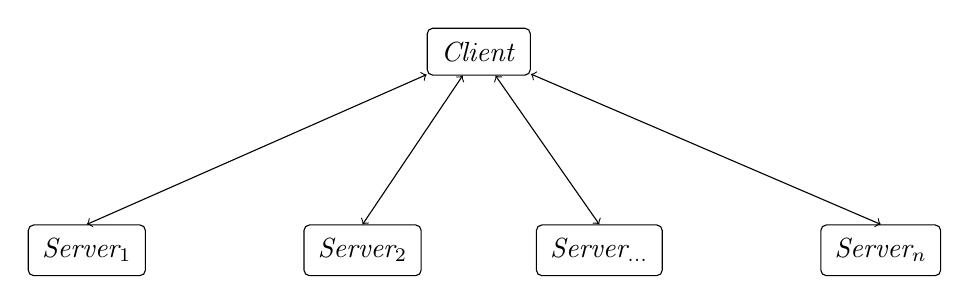
\begin{tikzpicture}[rounded corners=2pt,inner sep=5pt,node distance=2.0cm]
		\node [draw](client) { \textit{Client}};
		\node [inner sep=0pt, below=of client](aux) {\strut};
		\node [draw,left=.7cm of aux] (server2) {\textit{Server$_2$}};
		\node [draw,right=.7cm of aux] (server3) {\textit{Server$_{\ldots}$}};
		\node [draw,left=of server2] (server1) {\textit{Server$_1$}};
		\node [draw,right=of server3] (server4) {\textit{Server$_n$}};
		\foreach \n in {1,...,4}
			\draw [<->] (client) -- (server\n.north);
	\end{tikzpicture}
	\caption{System Design}\label{chapter:dist:design}
\end{figure}

The use of the terms \textit{client} and \textit{server} may sound a little different than what you may expect, but they aren't. A typical description of a system is that of a server with many connected clients, for example many web browsers and a single web server. In the model presented in this chapter, there is a single client, but many connected servers. If you think about the clients and servers, regardless of their number, they perform the same roles in both models. In the case of the clients, a web server or an interactive Mandelbrot application, they both respond to user inputs and make requests to a server, or servers. With respect to a server in a web system, the web server receives requests, performs computational tasks and returns those results to the client. The server in our system receives tasks, executes those tasks, and returns the results to the client. In other words, the use of the terms is the same, it is only the system topology that is different.

\FigureGeneral \ref{chapter:dist:model-figure} provides an overview of the system model. The client process accepts input from the user and generates compute tasks, it is the server(s) that perform the execution of the tasks. Rather than tasks being placed into a client thread pool as is done in the previous chapters, tasks are placed into a \textit{Global Task Queue} from which they are distributed throughout the connected compute servers. Immediately after making a successful connection, a compute server sends a set of task requests to the client (represented by the arrow from the compute server to the \textit{Task Request Queue}), indicating it is available to receive work. The \textit{Task Request Queue} holds the requests from the servers which get matches with waiting tasks. When a match is made, the task is transmitted to the compute server and placed in its \textit{Local Task Queue} (represented by the arrow from the client \textit{Global Task Queue} to the compute server \textit{Local Task Queue}) from which the server selects, executes the tasks, compiles the results, and returns the results back to the client.

\begin{figure}[H]
	\centering	
	\fbox
	{
		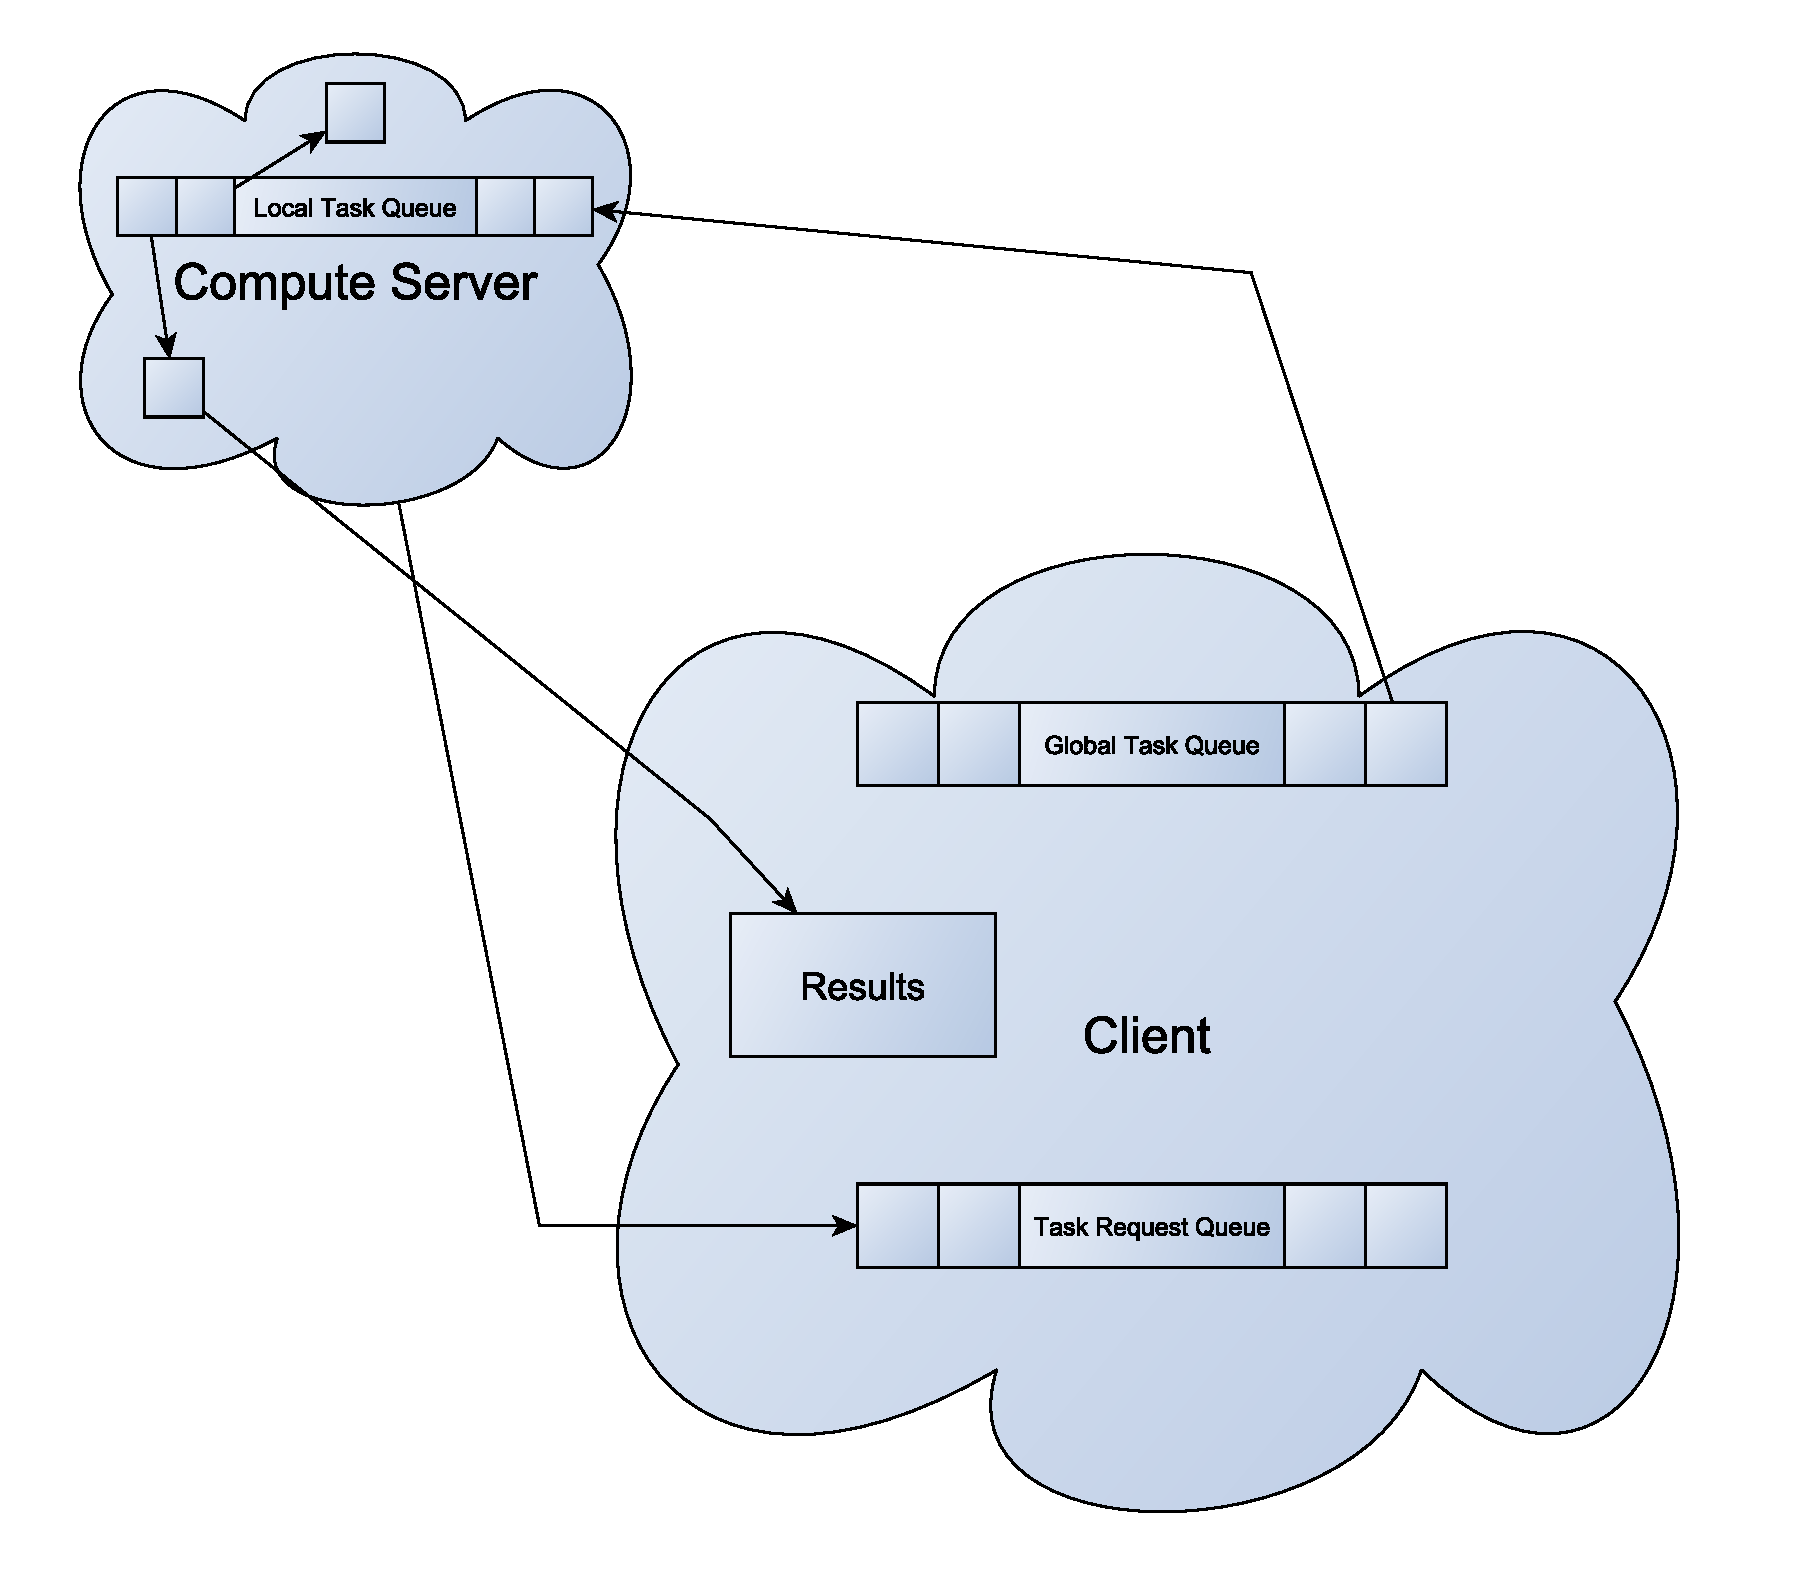
\includegraphics[width=4.5in, height=4.5in]{Images/Distributed-Model.pdf}
	}
	\caption{Distributed Model}
	\label{chapter:dist:model-figure}
\end{figure}

The small squares with arrows pointing to them on the compute server represent tasks that have been removed from the \textit{Local Task Queue} and are being executed. The arrow going from the small square on the compute server to the \textit{Results} box represents a task that has finished execution and its results being sent back to the client.

The model in this figure is only that, a model, the implementation details have additional complexity. The specifics of how this model is implemented are presented in the remainder of the chapter.

\FigureGeneral \ref{chapter:dist:communication-figure} shows the sequence of communication that takes place between the client and a server. The first step is for a server to initiate and establish a connection with the client. Upon successful connection, the server then sends a task request to the client, indicating it is available to perform work. When the client is ready to have a task computed, it sends a task to the server, the server computes the result, sends it back to the client, and immediately sends another task request indicating it can take on more work with the completion of the previous task. In the case the client is shutting down, it sends a termination message to all connected servers instructing them to gracefully shutdown.

\begin{figure}[H]
	\centering	
	\includegraphics[width=4.5in, height=4.5in]{Images/Distributed-Communication-Sequence.png}
	\caption{Distributed Communication}
	\label{chapter:dist:communication-figure}
\end{figure}

Not shown in this diagram, but implied, is once the client receives the results, it places them into the display buffer for immediate viewing; or in the case of a prime number, reports the result to the console upon receipt.

The core fundamental continues to hold true, decomposing a problem into computable tasks. The compute servers indicate their availability for work, ensuring the client only sends a task when it has available resources. Because of this, the system as a whole continues to exhibit a scalable nature by automatically load balancing the tasks over the connected compute servers. Because of the design and implementation groundwork laid in the first version of the application, all of the major components that ensure scalability are already in place, significantly easing the transition to a distributed framework, while maintaining the scalable nature.

\section{Networking Infrastructure} %Shared

Chapter \ref{chapter:networking} introduced the networking techniques used as the basic building blocks for distributed communication. The discussion was furthered in Chapter \ref{chapter:coding} with a description of how messages are coded and encoded for transmission between processes. This section continues the discussion by futher detailing the networking framework.

\subsection{Client \& Server Initialization}

The code presented in the previous chapters placed the basic application framework in a class named \texttt{ScalabilityApp}, the code associated with this chapter renames the class to \texttt{DistributedApp} to better reflect its nature. In addition to a new name, quite a bit of new code has been added. One of these new additions is the initialization of the Boost.Asio library's \texttt{io\_service}. This code is contained in the \texttt{DistributedApp::initialize} method, shown in \FigureCode \ref{chapter:dist:client-initialize}. Remember that the system is now composed of two processes, a client and server, this code is only part of the client process.

\begin{code}[caption={Client Initialization}, label=chapter:dist:client-initialize]
bool DistributedApp::initialize()
{
  using namespace boost::asio;
  m_threadWork = std::unique_ptr<io_service::work>
    (new io_service::work(m_ioService));
  for (auto thread : IRange<uint8_t>(1, 10))
  {
    m_threadsIO.push_back(std::unique_ptr<std::thread>(
      new std::thread(
        [this]()
        {
          m_ioService.run();
        })));
  }

  TaskRequestQueue::instance()->initialize(&m_ioService, &m_servers);

  waitOnConnection();

  return true;
}
\end{code}

The first part of this function creates the \texttt{io\_service}, along with assigning a pool of threads. The client will have potentially many connected compute servers, this allows many different connections to be serviced concurrently. An \texttt{io\_service::work} object is also created and associated with the \texttt{io\_service} to prevent it from terminating when there are no events on its request queue. The next step is to initialize the \texttt{TaskRequestQueue}, which needs to have access to the application \texttt{io\_service}; this singleton is fully discussed in Section \ref{chapter:dist:client}. The final step in the initialization is to begin waiting for connections from servers, which is described in the next section.

The server has an analogous initialization to the client, shown by the two code sections in \FigureCode \ref{chapter:dist:server-initialize}. It creates an \texttt{io\_service} queue, \texttt{io\_service::work} object, but only places a single thread on the \texttt{io\_service}. The server only ever communicates with the client, therefore the need to have more than one thread to handle network communication is not necessary. Following this, an instance of a class named \texttt{ComputeServer} is created and initialized. During its initialization a familiar \texttt{ThreadPool} is initialized, from which assigned tasks are associated and executed. Finally, the server enters a state where it initiates a connection to the client, this procedure is discussed in the next section.

\begin{code}[caption={Server Initialization}, label=chapter:dist:server-initialize]
int main(int argc, char* argv[])
{
  ...
  boost::asio::io_service ioService;
  boost::asio::io_service::work work(ioService);

  std::thread thread = std::thread(
    [&ioService]() 
    { 
        ioService.run();
    });

  ComputeServer server;
  server.initialize(ioService, ipClient, portClient);
  ...
}

void ComputeServer::initialize(
  boost::asio::io_service& ioService, 
  const std::string& ipClient, 
  const std::string& portClient)
{
  ThreadPool::instance()->initialize(&ioService);
  connectToClient(ioService, ipClient, portClient);
}
\end{code}

\subsection{Making a Connection}

Section \ref{chapter:networking:sockets:connection} of Chapter \ref{chapter:networking} provides the background on how to use Boost.Asio to initiate and accept networking connections. The code presented in this chapter follows those techniques, with a few minor differences owing to the context of the Mandelbrot viewing application.

The connection model used by the Mandelbrot application is to have the client wait for an incoming connection from a compute server. For the approach used in the Mandelbrot application, the servers must know the location of the client, but the client does not need advance knowledge of the servers. The start order of the processes doesn't matter. Upon start, a compute server continues to attempt making a connection to the client, retrying until either the connection is established or the process is manually terminated. Similarly, upon start, the client begins waiting for incoming connections, and allowing them to be made at any time during the application lifetime, not only during an initialization phase. This allows the client to take advantage of ever more computing resources over time. The code presented in this chapter does not discuss how to handle servers that disconnect or fail while the client is alive; a topic complex enough to require its own discussion, and tackled in Chapter \ref{chapter:ft}.

The server code for initiating a connection with the client is found in \FigureCode \ref{chapter:dist:init-connect}. The first part of the method is almost exactly as found in Section \ref{chapter:networking:init-connection} of Chapter \ref{chapter:networking}. The one difference is the use of the blocking \texttt{connect} instead of the non-blocking \texttt{async\_connect}. The reason for this is that the server doesn't need to do anything else while waiting for the connection to complete, therefore, the code is simplified by using a blocking call.

\begin{code}[caption={Initiating A Connection}, label=chapter:dist:init-connect]
void ComputeServer::connectToClient(
  boost::asio::io_service& ioService, 
  const std::string& ipClient, 
  const std::string& portClient)
{
  ip::tcp::resolver resolver(ioService);
  ip::tcp::resolver::query query(ipClient, portClient);
  ip::tcp::resolver::iterator iterator = resolver.resolve(query);

  bool done = false;
  while (!done)
  {
    auto socket = std::make_shared<tcp::socket>(ioService);
    boost::system::error_code error;
    boost::asio::connect(*socket, iterator, error);
    if (!error)
    {
      done = true;
      waitOnTask(socket);
      unsigned int count = std::max(
        1u, 
        std::thread::hardware_concurrency()) * 2;
      for (auto core : IRange<unsigned int>(1, count))
      {
        ioService.post(
          [socket]()
          {
            Messages::TaskRequest command;
            command.send(socket);
          });
      }
    }
  }
}
\end{code}

Once the \texttt{connect} method returns without error, \texttt{done} is set to \texttt{true} to indicate a successful connection has been made and the connection loop can end. Next, a call to the non-blocking \texttt{waitOnTask} method is made. This method, detailed in Section \ref{chapter:dist:network:receive-messages}, waits for task messages from the client. The final step is to send a number of task requests to the client. Each request indicates the availability of enough resources to compute one task. This is done by creating a bunch of \texttt{TaskRequest} messages and sending them over the connected socket.

The reason for sending more task requests than the number of available cores is to allow for I/O operations to be taking place while other tasks are executing. Consider that a system can be sending a task request, receiving a task, sending the results from executing a task, and executing several other tasks, all at the same time. On the other hand, only a single thread is assigned to the \texttt{io\_service}, for a number of reasons. Foremost is that there is only one network card, and only one connection to a single client. Secondly, the expectation with the server is for it to be compute bound, working on tasks, instead of being I/O bound, sending and receving messages over the network. Time spent computing should dominate the time spent performing I/O, if at all possible. In order to more effectively keep the CPU cores fully utilized, it is necessary to have at least one task waiting for execution as soon as one completes. This means the number of task requests must exceed the number of available CPU cores by enough to prevent the system from waiting for I/O to complete to begin execution of the next task.

The other side of the connection is the client, which waits for an incoming connection request; the code shown in \FigureCode \ref{chapter:dist:wait-connect} demonstrates this. Again, the code for the client follows the pattern described in Section \ref{chapter:networking:accept-connection} of Chapter \ref{chapter:networking}. When a successful a connection is made, a \texttt{Server} instance is created and added to the list of known servers. This is followed by a call to the non-blocking method \texttt{waitOnMessage}, described in Section \ref{chapter:dist:network:receive-messages}.

\begin{code}[caption={Waiting For Connection}, label=chapter:dist:wait-connect]
void DistributedApp::waitOnConnection()
{
  auto socket = std::make_shared<ip::tcp::socket>(m_ioService);
  m_acceptor.async_accept(*socket,
    [this, socket](const boost::system::error_code& error)
    {
      if (!error)
      {
        Server server(socket);
        m_servers.add(server);
        waitOnMessage(server.id);
      }
      waitOnConnection();
  });
}
\end{code}

The \texttt{Server} struct is used by the client to maintain connection information about a connected server. Each instance is also assigned a unique identifier that is used as the key for reference in a hash table in the \texttt{ServerSet} class. The struct also holds a pointer to the socket over which communication takes place. In order to ensure valid synchronization of threads communicating with each server, as described in Chapter \ref{chapter:networking}, each server is given its own \texttt{strand}; all communication requests with the server are posted to this \texttt{strand}. The code for this struct is found in \FigureCode \ref{chapter:dist:server-struct}.

\begin{code}[caption={\texttt{Server} Struct}, label=chapter:dist:server-struct]
struct Server
{
  Server() {} 
  Server(boost::asio::io_service& ioService)
  {
    static ServerID_t newId = 0;
    this->id = newId++;
    this->strand = std::make_shared<boost::asio::strand>(
        socket->get_io_service());
  }

  ServerID_t id;
  std::shared_ptr<ip::tcp::socket> socket;
  std::shared_ptr<boost::asio::strand> strand;
  std::array<uint8_t, 1> messageType;
};
\end{code}

Associated with the \texttt{Server} struct is a class named \texttt{ServerSet} which is used as a container to maintain details of all connected servers. This class primarily provides synchronized access to the list of available servers. The \texttt{add}, \texttt{get}, and \texttt{exists} are simple helper methods that control, and synchronize, access to the \texttt{std::unordered\_map} of \texttt{Server} structs. The declaration for this class is shown in \FigureCode \ref{chapter:dist:server-set}.

\begin{code}[caption={\texttt{ServerSet} Class}, label=chapter:dist:server-set]
class ServerSet
{
public:
  void add(Server server);
  boost::optional<Server&> get(ServerID_t id);
  bool exists(ServerID_t id);
  std::unordered_map<ServerID_t, Server> getServers();

private:
  std::unordered_map<ServerID_t, Server> m_servers;
  std::mutex m_mutex;
};
\end{code}

\subsection{Command Pattern}\label{chapter:dist:network:command-pattern}

This distributed application takes advantage of a design pattern known as the \textit{Command Pattern}\footnote{http://en.wikipedia.org/wiki/Command\_pattern} to reduce code complexity and improve it for future maintenance, as additional messages are added to the system. The design pattern is used to associate a message type with a handler function or method. The implementation uses a hash table (\texttt{std::unordered\_map}), where a message type is used as the key and the value is a \texttt{std::function}; which is invoked when the message type is received. The hash table type for the client is shown in \FigureCode \ref{chapter:dist:client-pattern-type}, and the server type is shown in \FigureCode \ref{chapter:dist:server-pattern-type}.

\begin{code}[caption={Client Command Pattern Type}, label=chapter:dist:client-pattern-type]
std::unordered_map<
  Messages::Type, 
  std::function<void (ServerID_t)>>
\end{code}

\begin{code}[caption={Server Command Pattern Type}, label=chapter:dist:server-pattern-type]
std::unordered_map<
  Messages::Type, 
  std::function<void (std::shared_ptr<ip::tcp::socket>)>>
\end{code}

For the client, the function handler accecpts a \texttt{ServerID\_t} as a parameter, which is the unique identifier for the server from which the message originated. This parameter is then used to lookup the server from the \texttt{ServerSet} and retrieve the socket connection for communication. For the server, the function handler accepts the socket over which communication to the client takes place. There is only one socket between the server and client, therefore no need to manage and lookup different sockets for different routes of communication at the server.

The client and server both declare a member variable named \texttt{m\_messageCommand} of their command pattern types in the \texttt{DistributedApp} and \texttt{ComputeServer} classes, respectively; I refer to these as \textit{command maps}. During application initialization, the command maps are initialized with the different types of messages that can be received and their associated handlers. The initialization code for the client is show in \FigureCode \ref{chapter:dist:client-pattern-init}.

\begin{code}[caption={Client Command Map Initialization}, label=chapter:dist:client-pattern-init]
void DistributedApp::prepareCommandMap()
{
  m_messageCommand[Messages::Type::TaskRequest] = 
    [this](ServerID_t serverId) 
    { 
      processTaskRequest(serverId); 
    };
  m_messageCommand[Messages::Type::MandelResult] = 
    [this](ServerID_t serverId) 
    { 
      processMandelResult(serverId); 
    };
  m_messageCommand[Messages::Type::NextPrimeResult] = 
    [this](ServerID_t serverId) 
    { 
      processNextPrimeResult(serverId); 
    };
}
\end{code}

The \texttt{prepareCommandMap} method associates a lambda function with each of the types of messages it may receive from a compute server. The lambda has the same signature as the \texttt{std::function} defined as part of the \texttt{m\_messageCommand} type. Upon invocation, the lambda simply makes a call to an instance method that performs the actual work of handling the message type. The initialization of the command map for the server looks the same as the client, except that it responds to different message types and invokes different handlers.

The code in \FigureCode \ref{chapter:dist:pattern-sample} demonstrates how to use the command map to invoke the handler for a specific message. The \texttt{[Messages::Type::TaskRequest]} part of the statement searches the hash table for the entry corresponding to that key, which is a function. Then, the \texttt{(serverId)} part of the statement invokes the returned function.

\begin{code}[caption={Command Map Invocation}, label=chapter:dist:pattern-sample]
m_messageCommand[Messages::Type::TaskRequest](serverId);
\end{code}

There command map code for the server is able to be somewhat simplified over the client code because the same thing is done for all messages except for one. Because of this, the code for the server can take advantage of generic programming by having a templated \texttt{processTask} function that does the same thing for every message and task type combination. The code for this function is shown in \FigureCode \ref{chapter:dist:server-processtask}. This function simply reads the remainder of the message from the socket, then places the task onto the local \texttt{ThreadPool} for execution.

\begin{code}[caption={Server Templated \texttt{processTask}}, label=chapter:dist:server-processtask]
template <typename Message, typename Task>
void processTask(std::shared_ptr<ip::tcp::socket> socket)
{
  Message message;
  message.read(socket);
  std::shared_ptr<Tasks::Task> task = std::make_shared<Task>(socket, message);

  ThreadPool::instance()->enqueueTask(task);
}
\end{code}

The initialization of the server command map makes use of the templated \texttt{processTask} function. As this method is used, the message and task types are specified as template parameters for the \texttt{processTask} function, as demonstrated in \FigureCode \ref{chapter:dist:server-pattern-init}. There is one exception to the messages received at the server, and that is the terminate command. A \texttt{TerminateCommand} message is not a computational task, therefore it doesn't belong on the \texttt{ThreadPool}, it is a message instructing the server process to perform a graceful shutdown. Because of this, a specific function is used to handle that message, \texttt{processTerminateCommand}, which is reflected in the initialization of the command map.

\begin{code}[caption={Server Command Map Initialization}, label=chapter:dist:server-pattern-init]
void ComputeServer::prepareCommandMap()
{
  m_messageCommand[Messages::Type::MandelMessage] = 
    [this](std::shared_ptr<ip::tcp::socket> socket)
    {
      processTask<Messages::MandelMessage, Tasks::MandelTask>(socket);
    };
  m_messageCommand[Messages::Type::NextPrimeMessage] = 
    [this](std::shared_ptr<ip::tcp::socket> socket)
    {
      processTask<Messages::NextPrimeMessage, Tasks::NextPrimeTask>(socket);
    };
  m_messageCommand[Messages::Type::TerminateCommand] =
    [this](std::shared_ptr<ip::tcp::socket> socket)
    {
      processTerminateCommand(socket);
    };
}
\end{code}

\subsection{Receiving Messages}\label{chapter:dist:network:receive-messages}

The technique for message encoding before sending was presented in Chapter \ref{chapter:coding}, along with how a message is read and decoded once the message type is known. But we still need to understand how an application waits for messages to arrive, determines the message type in order to create the correct message instance, and then passed off to be read and decoded.

\FigureCode \ref{chapter:dist:client:wait-message} shows the \texttt{waitOnMessage} that is called whenever a compute server makes a connection to the client. Almost all of the code is a lambda that is passed as a parameter to the non-blocking \texttt{async\_receive} call. This becomes a handler on the \texttt{io\_service} that is invoked whenever a message is received over this socket. Think carefully about this, for each connected server there is a pending receive handler associated with the socket connection; it is not a single handler for all servers, it is multiple handlers, one for each connected server/socket.

\begin{code}[caption={Client \texttt{waitOnMessage}}, label=chapter:dist:client:wait-message]
void DistributedApp::waitOnMessage(ServerID_t serverId)
{
  boost::optional<Server&> server = m_servers.get(serverId);
  server->socket->async_receive(boost::asio::buffer(server->messageType),
    [this, serverId, server]
    (const boost::system::error_code& error, std::size_t bytes)
    {
      if (!error && bytes > 0)
      {
        Messages::Type type = 
          static_cast<Messages::Type>(server->messageType[0]);
        m_messageCommand[type](serverId);
        waitOnMessage(serverId);
      }
    });
}
\end{code}

The \texttt{Server} structure defines a single byte \texttt{std::array} that is used as a buffer into which the first byte of a message is received. This array is passed as the first parameter to the \texttt{async\_recieve} call. The second parameter is the lambda to invoke when the byte is received. Section \ref{chapter:coding:send-receive} of Chapter \ref{chapter:coding} showed that the first byte sent as part of a message is the unique message type. The client can receive three different messages from the server: a request for a task, results for a Mandelbrot task, and the results from a prime number task. These three messages correspond to the following enumeration types: \texttt{Messages:Type::TaskRequest}, \texttt{Messages::Type::MandelResult}, \texttt{Messages::Type::NextPrimeResult}. These are the three message handlers registered with the command map presented in Section \ref{chapter:dist:network:command-pattern}.

As a bit of sanity checking, the first part of the lambda checks to see if an error occurred on the socket, causing the handler to be invoked. If no error occurred, the rest of the message is processed. The next bit of code casts the received byte to a \texttt{Messages::Type} allowing it to be used as the key for invoking the message handler on the \texttt{m\_messageCommand} hash table. It is during the this call that the rest of the message is read from the socket, decoded, and processed. Once the call on the command map has completed, a new call to \texttt{waitOnMessage} is made in order to place a new handler on the \texttt{io\_service} to respond the next message received.

An example command map handler is shown in \FigureCode \ref{chapter:dist:client:process-prime}. This method is invoked when a prime number result message is received from a compute server. The lambda registered in the \texttt{waitOnMessage} reads the first byte of the message, then based upon that message, this handler is invoked. This handler creates an instance of the \texttt{NextPrimeResultMessage} class, which then finishes reading the data from the socket and decodes the results into the class members.

\begin{code}[caption={Process Prime Result}, label=chapter:dist:client:process-prime]
void DistributedApp::processNextPrimeResult(
    ServerID_t serverId)
{
  Messages::NextPrimeResultMessage taskResult;
  taskResult.read(m_servers.get(serverId)->socket);

  m_lastPrime = taskResult.getNextPrime();
  m_reportPrime = true;
  std::shared_ptr<Tasks::NextPrimeTask> task = 
    std::make_shared<Tasks::NextPrimeTask>(
      taskResult.getNextPrime(), 
      Tasks::Task::Priority::Three);
  TaskRequestQueue::instance()->enqueueTask(task);
}
\end{code}

With the result message processed, the handler remembers the newly generated prime number to the private class member \texttt{m\_lastPrime}. Next, the \texttt{m\_reportPrime} boolean is set to \texttt{true}, which tells the application to display the \texttt{m\_lastPrime} value to the console. Finally, a new \texttt{NextPrimeTask} is created and placed on the \texttt{TaskRequestQueue}. This function completes the prime number computation loop, keeping the computation ongoing throughout the lifetime of the application.

The compute server is substantially similar to the client. It makes a call to the non-blocking \texttt{async\_receive}, passing a single byte buffer as the first parameter and a lambda to be invoked upon receipt of the byte. Once again, the byte is converted to a \texttt{Messages::Type}, the command map handler invoked, and then a new call to \texttt{waitOnTask} is made. The code for this method is found in \FigureCode \ref{chapter:dist:server:wait-task}.

\begin{code}[caption={Server \texttt{waitOnTask}}, label=chapter:dist:server:wait-task]
void ComputeServer::waitOnTask(
    std::shared_ptr<ip::tcp::socket> socket)
{
  socket->async_receive(boost::asio::buffer(m_messageType),
    [this, socket](const boost::system::error_code& error, std::size_t bytes)
    {
      if (!error)
      {
        Messages::Type type = static_cast<Messages::Type>(m_messageType[0]);
        m_messageCommand[type](socket);
        waitOnTask(socket);
      }
    });
}
\end{code}

\subsection{Sending Tasks}\label{chapter:dist:network:send-task}

The \texttt{Task} is updated to reflect the nature of a distributed application. A task now knows how to send itself to a compute server via a socket, along with knowing how to return a computed result back to the client. These new capabilities have changed the application interface through the addition of a new \texttt{send} method, and a change in the approach to how the \texttt{complete} method is implemented. \FigureCode \ref{chapter:dist:task-decl} shows a portion of the revised \texttt{Task} class delcaration.

\begin{code}[caption={Revised \texttt{Task} Declaration}, label=chapter:dist:task-decl]
class Task
{
public:
  void send(
    std::shared_ptr<ip::tcp::socket> socket, 
    boost::asio::strand& strand);

  void complete(boost::asio::io_service& ioService);

protected:
  virtual std::shared_ptr<Messages::Message> getMessage() = 0;
  virtual void completeCustom(boost::asio::io_service& ioService) = 0;
};
\end{code}

The new \texttt{send} method has the responsibility to send a task message to a connected server, using the socket and strand passed to it. The implementation for this method is almost trivial, as shown in \FigureCode \ref{chapter:dist:task:send}. The first thing the code does is to call into the derived class \texttt{getMessage} method to obtain a fully formed \texttt{Message} that is then sent to the compute server.

\begin{code}[caption={\texttt{Task::send} Implementation}, label=chapter:dist:task:send]
void Task::send(
  std::shared_ptr<ip::tcp::socket> socket, 
  boost::asio::strand& strand)
{
  auto message = getMessage();
  message->send(socket, strand);
}
\end{code}

Notice that \texttt{Task::getMessage} is a pure virtual method, forcing derived \texttt{Task} classes to provide an implementation. The only thing this method needs to do is to construct and return a shared pointer to a \texttt{Message} class that represents the work to be done at the compute server. An example implementation for a \texttt{getMessage} is shown in \FigureCode \ref{chapter:dist:mandel-message:get-message}. The code simply creates and returns a shared pointer to an instance of a \texttt{MandelMessage} using the attribute values of the \texttt{MandelTask} instance.

\begin{code}[caption={\texttt{MandelTask::getMessage} Implementation}, label=chapter:dist:mandel-message:get-message]
std::shared_ptr<Messages::Message> MandelTask::getMessage()
{
  return 
    std::shared_ptr<Messages::MandelMessage>(
      new Messages::MandelMessage(
        m_id, 
        m_startRow, m_endRow, 
        m_sizeX, 
        m_startX, m_startY, 
        m_deltaX, m_deltaY, 
        m_maxIterations));
}
\end{code}

\section{Client Notes}\label{chapter:dist:client}

The client is the Windows part of the distributed application. It is responsible for the display of the Mandelbrot image, along with display of the prime number generation results. In the same way as the previous chapters, the client is responsible for generating the tasks that need to be computed, whether tasks for computing the Mandelbrot set or tasks for computing the next prime number. The difference now is that the client does not contain any code to perform those computations, it only generates the tasks and distributes them to the connected servers. The remainder of this section details how tasks are distributed to the connected servers, along with describing how a graceful shutdown of the client is performed.

\subsection{Matching Tasks \& Requests}

Because the application is now composed of multiple processes, all executing on different computers, it requires a change in how selecting tasks for computation is handled. In the first three versions of the application, tasks were placed on a thread pool. The tasks were then grabbed by an available thread and executed. With the distributed application, the client no longer has that same thread pool, instead, the thread pool is on the server processes, where the tasks are executed. The tasks are generated by the client Mandelbrot application. As described in the first part of the chapter, servers send task requests to the client, and those requests are matched with waiting tasks. This matching takes place on a new singleton object as part of the client, the \texttt{TaskRequestQueue}.

The declaration for the \texttt{TaskRequestQueue} is shown in \FigureCode \ref{chapter:dist:task-request-queue}. This class is immediately familiar because of similarities it shares with the \texttt{ThreadPool}. It is implemented as a singleton, because there should only be one in existence for any application, along with making it globally accessible. Secondly, it has the same \texttt{enqueueTask} method and supporting class members. It diverges in that it is not a thread pool, the addition of the \texttt{enqueueRequest} method, and the distribution algorithm that matches tasks with requests and distributes them to the servers.

\begin{code}[caption={\texttt{TaskRequestQueue} Declaration}, label=chapter:dist:task-request-queue]
class TaskRequestQueue
{
public:
  static std::shared_ptr<TaskRequestQueue> instance();

  void initialize(
    boost::asio::io_service* ioService, 
    ServerSet* servers);
  void terminate();
  void enqueueRequest(ServerID_t request);
  void enqueueTask(std::shared_ptr<Tasks::Task> task);

protected:
  TaskRequestQueue();

private:
  static std::shared_ptr<TaskRequestQueue> m_instance;
  boost::asio::io_service* m_ioService;
  ServerSet* m_servers;

  std::queue<ServerID_t> m_queueRequest;
  std::mutex m_mutexRequest;
  std::condition_variable m_eventRequest;
  std::mutex m_mutexEventRequest;

  ConcurrentPriorityQueue<std::shared_ptr<Tasks::Task>, TaskCompare> m_queueTasks;
  std::condition_variable m_eventTask;
  std::mutex m_mutexEventTask;

  std::shared_ptr<std::thread> m_distributer;
  bool m_distributerDone;

  void distribute();
  void fillRequest(std::shared_ptr<Tasks::Task> task);
};
\end{code}

As indicated in the description above, the \texttt{TaskRequestQueue} has two containers that hold the task requests and tasks. The task requests are stored in the \texttt{m\_queueRequest} member, which is a \texttt{std:queue}. Just like the thread pool from the chapter on priority, the tasks are stored in a new container, a \texttt{ConcurrentPriorityQueue}. This container is a simple thread-safe wrapper around the \texttt{std::priority\_queue}. Each of these containers are associated with a condition variable, \texttt{m\_eventRequest} and \texttt{m\_eventTask} respectively, that are signaled when an item is added.

When the singleton is first used, it creates a private \texttt{m\_distributer} thread. \FigureCode \ref{chapter:dist:trq:instance} shows the \texttt{instance} method where the thread is created. The purpose of this thread is to respond to incoming task requests and tasks, matching and sending them off to be computed. The matching algorithm is discussed later in this section.

\begin{code}[caption={\texttt{TaskRequestQueue::instance}}, label=chapter:dist:trq:instance]
std::shared_ptr<TaskRequestQueue> TaskRequestQueue::instance()
{
  if (m_instance) return m_instance;

  m_instance = std::shared_ptr<TaskRequestQueue>(new TaskRequestQueue());

  m_instance->m_distributer = 
    std::make_shared<std::thread>(&TaskRequestQueue::distribute, m_instance);

  return m_instance;
}
\end{code}

The \texttt{TaskRequestQueue} exposes two primary public methods as its application interface, \texttt{enqueueRequest} and \texttt{enqueueTask}. The code for these methods is shown in \FigureCode \ref{chapter:dist:trq:enqueue}. These methods work in the same way, adding either a task request or task to the appropriate container. The \texttt{enqueueRequest} method is used to add incoming task requests from servers. The \texttt{enqueueTask} method is used to add tasks to be computed from the client. Each of these methods signal condition variables that release the thread that attempts to match a request and task. The \texttt{enqueueRequest} method uses a mutex to protect the \texttt{m\_queueRequest} container because it is a non-thread safe container, a \texttt{std::queue}. No mutex protection is needed in \texttt{enqueueTask} because \texttt{m\_queueTasks} is a thread safe container.

\begin{code}[caption={\texttt{TaskRequestQueue} Declaration}, label=chapter:dist:trq:enqueue]
void TaskRequestQueue::enqueueRequest(
    ServerID_t request)
{
  std::lock_guard<std::mutex> lock(m_mutexRequest);

  m_queueRequest.push(request);
  m_eventRequest.notify_all();
}

void TaskRequestQueue::enqueueTask(std::shared_ptr<Tasks::Task> task)
{
  m_queueTasks.enqueue(task);
  m_eventTask.notify_all();
}
\end{code}

The heart of the \texttt{TaskRequestQueue} is found in the \texttt{distribute} method, shown in \FigureCode \ref{chapter:dist:trq:distribute}. This is the initial method called when the \texttt{TaskRequestQueue} thread is started. The purpose of this method is to remove tasks from the \texttt{m\_queueTasks} container and then call \texttt{fillRequest} to match them with a waiting task request. As long as tasks are available, they are removed from the priority queue. Just like the standalone priority application from earlier in the book, tasks of all priorities at, or below, the specified level are checked. When no tasks are available, the method enters an efficient wait state, waiting for the \texttt{m\_eventTask} condition variable to be signaled.

\begin{code}[caption={Task Distribution}, label=chapter:dist:trq:distribute]
void TaskRequestQueue::distribute()
{
  while (!m_distributerDone)
  {
    auto task = m_queueTasks.dequeue();
    if (task)
    {
      fillRequest(task.get());
    }
    else
    {
      std::unique_lock<std::mutex> lock(m_mutexEventTask);
      m_eventTask.wait(lock);
    }
  }
}
\end{code}

Once a task is selected, the \texttt{fillRequest} method is called to match it with a task request and send it to the associated compute server; the code for this method is shown in \FigureCode \ref{chapter:dist:trq:fill-request}. This method doesn't return until the task is matched with a request. Even though it is a blocking call, it stays in an efficient loop until a task request is available. This is done by first checking the \texttt{m\_queueRequest} container for a task request. If one is found, the unique id of the server is captured and the loop is ended. If no task request is available, the method enters an efficient wait state on the \texttt{m\_eventRequest} condition variable. When a new task request comes in, the condition variable is signaled and the request container is checked again.

\begin{code}[caption={Filling Task Requests}, label=chapter:dist:trq:fill-request]
void TaskRequestQueue::fillRequest(
  std::shared_ptr<Tasks::Task> task)
{
  ServerID_t serverId = 0;
  bool done = false;
  while (!done)
  {
    std::lock_guard<std::mutex> lockRequest(m_mutexRequest);
    if (!m_queueRequest.empty())
    {
      serverId = m_queueRequest.front();
      m_queueRequest.pop();
      done = true;
    }
    if (!done)
    {
      std::unique_lock<std::mutex> lock(m_mutexEventRequest);
      m_eventRequest.wait(lock);
    }
  }

  m_ioService->post(
    [this, serverId, task]()
    {
      task->send(
        m_servers->get(serverId)->socket, 
        *m_servers->get(serverId)->strand);
    });
}
\end{code}

Once a task request and a task are matched, the loop ends and the task is sent to the compute server. This is done by posting an event to the main application \texttt{io\_service} queue to call the \texttt{Task::send} method.

\subsubsection{Tasks \& Task Requests}

Tasks are placed onto the \texttt{TaskRequestQueue} in the same way as was done using the \texttt{ThreadPool} from previous chapters. The big change introduced with this chapter is distributing those tasks among the various connected computers. This is done, as already described, by matching task requests with tasks.

Task requests are sent from each connected server to the client. The code shown in \FigureCode \ref{chapter:dist:task-request-message} shows the class used to represent the message sent from a server to a client that it can accept a task. The only content of this message is its type, that is enough to indicate its purpose. This class must override the \texttt{encodeMessage} and \texttt{decodeMessage} methods because they are virtual in the base \texttt{Message}, but there is nothing do because of no additional content in the message.

\begin{code}[caption={\texttt{TaskRequest} Message}, label=chapter:dist:task-request-message]
class TaskRequest : public Message
{
public:
  TaskRequest() :
    Message(Messages::Type::TaskRequest)
  {
  }

protected:
  virtual void encodeMessage() override {}
  virtual void decodeMessage() override {}
};
\end{code}

The client needs to be able to know what to do when this message is received. Section \ref{chapter:dist:network:command-pattern} described the Command Pattern infrastructure used to register and handle incoming messages, the \texttt{TaskRequest} message needs to be registered into this pattern. The code shown in \FigureCode \ref{chapter:dist:command:taskrequest} shows the code used to register a handler for the \texttt{TaskRequest} message. When invoked, the handler makes a call to \texttt{processTaskRequest}; the code for this method is shown in \FigureCode \ref{chapter:dist:process:taskrequest}.

\begin{code}[caption={\texttt{TaskRequest} Message Handler}, label=chapter:dist:command:taskrequest]
m_messageCommand[Messages::Type::TaskRequest] = 
  [this](ServerID_t serverId) 
  {
    processTaskRequest(serverId);
  };
\end{code}

The \texttt{processTaskRequest} method follows the same pattern as all message handlers. The first step is to finish reading the message, by calling the overloaded message \texttt{read} method (which in this case actually does nothing, because there is no more data to read). The next step is to perform any custom logic based upon receipt of this message. In the case of a \texttt{TaskRequest} message, the custom logic is to make a call to the \texttt{TaskRequestQueue::enqueueRequest} method, indicating the connected server is available to receive a new task.

\begin{code}[caption={\texttt{processTaskRequest}}, label=chapter:dist:process:taskrequest]
void DistributedApp::processTaskRequest(ServerID_t serverId)
{
  Messages::TaskRequest taskRequest;
  taskRequest.read(m_servers.get(serverId)->socket);
  TaskRequestQueue::instance()->enqueueRequest(serverId);
}
\end{code}

\subsection{Client Termination}

The client application is terminated when the user presses the <ESC> key. When pressed, the Windows message loop terminates and the \texttt{DistributedApp::terminate} method is called, shown in \FigureCode \ref{chapter:dist:client-termination}. This method performs a graceful shutdown of the client application.

\begin{code}[caption={Client Termination}, label=chapter:dist:client-termination]
void DistributedApp::terminate()
{
  m_running = false;
  TaskRequestQueue::instance()->terminate();

  std::atomic<std::size_t> sendRemaining = m_servers.getServers().size();
  for (auto server : m_servers.getServers())
  {
    Messages::TerminateCommand terminate;
    terminate.send(server.second.socket,
      [&sendRemaining](bool)
      {
        sendRemaining--;
      });
  }

  while (sendRemaining > 0)
    ;

  for (auto server : m_servers.getServers())
  {
    server.second.socket->close();
  }

  m_ioService.stop();

  for (auto& thread : m_threadsIO)
  {
    thread->join();
  }
}
\end{code}

The first step in terminating is to internally indicate to the client that it should no longer continue running, this is performed by setting the \texttt{m\_running} flag to \texttt{false}. This flag is tested by the \texttt{waitOnConnection} and \texttt{waitOnMessage} methods to see if they should continue working or not. Once set to \texttt{false}, those methods will not make any further calls to themselves when the \texttt{io\_service} handler is invoked. When \texttt{m\_ioService.stop()} is called, this causes any pending handlers to be invoked, but with an error condition indicated. This is how these methods gracefully exit.

The next step is to perform a graceful shutdown of the \texttt{TaskRequestQueue}. The \texttt{TaskRequestQueue} is the client component responsible for matching tasks and requests, it needs to be terminated in order to stop distributing tasks to workers. The \texttt{TaskRequestQueue::terminate} method is shown in \FigureCode \ref{chapter:dist:trq-termination}. This code signals the \texttt{m\_eventTask} and \texttt{m\_eventRequest} condition variables so that they will come out of their waiting states and terminate. The final statement performs a join operation on the distributor to guarantee it has completed before exiting this method.

\begin{code}[caption={TaskRequestQueue Termination}, label=chapter:dist:trq-termination]
void TaskRequestQueue::terminate()
{
  m_distributerDone = true;
  m_eventTask.notify_all();
  m_eventRequest.notify_all();

  m_distributer->join();
}
\end{code}

With the \texttt{TaskRequestQueue} terminated, we know there are no more tasks being sent to the connected compute servers. This makes it safe to now send a message to each of the connected compute servers to terminate. A special message is sent to each server, \texttt{Messages::TerminateCommand}. Upon receipt of this message a server will perform a graceful shutdown.

During the send of the \texttt{Messages::TerminateCommand} messages, a short lambda is passed in to be called once the send has completed. This lambda keeps track of how many more \texttt{Messages::TerminateCommand} messages remain to be sent. Immediately below the loop to send these messages, a busy loop is entered, this loop blocks until all of the \texttt{Messages::TerminateCommand} messages have been sent. The use of a busy loop in this context is acceptable because we aren't concerned with performance. It would be possible to make use of a \texttt{condition\_variable} and some other logic to create an efficient wait state, but doing so results in unnecessarily complex code for no benefit.

Once the termination messages are sent to the servers, it is now safe to close the socket connections to each of those servers. Once those connections are closed, no more work can be sent, therefore it is now safe to stop the \texttt{io\_service}. As noted above, when this is stopped, all pending handlers are invoked, allowing them to gracefully stop.

The last step is to wait for the threads associated with the \texttt{io\_service} to complete. A join is performed on each of those threads and once they have all completed, the application ends execution.

\subsection{Use of \texttt{boost::optional} in \texttt{ConcurrentPriorityQueue}}\label{chapter:dist:section:concurrent-priorityqueue}

Mostly as a side note to describe the use of \texttt{boost::optional}, the code in \FigureCode \ref{chapter:dist:concurrent-pq} shows the \texttt{dequeue} implemention of the new \texttt{ConcurrentPriorityQueue} class. Because the \texttt{boost} library is now being used in the project, the \texttt{dequeue} method has been written to take advantage of \texttt{boost::optional} as part of the return type. This allows the return type to indicate a \texttt{true/false} whether or not a value was returned, and then the value can be obtained. Using \texttt{boost::optional} eliminates the need for any kind of \textit{sentinal} values indicating whether a value is valid or not; the value and existence of the value are now managed separately.

\begin{code}[caption={\texttt{ConcurrentPriorityQueue::dequeue}}, label=chapter:dist:concurrent-pq]
boost::optional<T> dequeue()
{
  std::lock_guard<std::mutex> lock(m_mutex);

  boost::optional<T> item;
  auto itr = m_queue.begin();
  if (!m_queue.empty())
  {
    item = m_queue.top();
    m_queue.pop();
  }

  return item;
}
\end{code}

Refer back to \FigureCode \ref{chapter:dist:trq:distribute} and notice the \texttt{task} variable. The use of \texttt{auto} hides the type, but it is a \texttt{boost::optional} around a \texttt{std::shared\_ptr}. The \texttt{boost::optional} part of the type is first tested to see if a value exists in the return, and if it does, the \texttt{task.get()} call returns the underlying \texttt{std::shared\_ptr}. This provides a clean separation of the return value from whether or not there is a return value, along with having a natural way (a boolean test) to test for the existence of a value.

\section{Server Notes}

The server's purpose is to perform the heavy computational lifting for the distributed application. With respect to the single system examples from the previous chapters, the server contains all of the task computation code, but none of the user interface. Most of the server code has already been discussed earlier in this chapter, leaving only a couple small pieces left to discuss. The first is how the server computes and then returns results back to the client. The second is how the server performs a graceful shutdown.

The server component of the system is a new process, it has no user interface, therefore, it is written as a console only application. Because it is a console application, unlike the client which is Windows only, this code compiles and runs just fine on Windows, Linux, Mac OS X, or any other platform with a compliant C++11 compiler and ability to compile Boost.Asio.

\subsection{Computing \& Returning Results}

Section \ref{chapter:dist:network:send-task} discussed how tasks are sent from the client to the servers. Once a server receives a task, it is placed on the server's \texttt{ThreadPool} where it will be handled by one of the worker threads. The logic for the \texttt{WorkerThread::run} method is exactly the same as with the priority system described in Chapter \ref{chapter:scalable-priority} and Section \ref{chapter:priority:impl:worker-thread}. What is different is the implementation of the \texttt{complete} method of the task. The code for the revised \texttt{complete} method is shown in \FigureCode \ref{chapter:dist:task-complete}.

\begin{code}[caption={Distributed \texttt{Task::complete} Method}, label=chapter:dist:task-complete]
void Task::complete(boost::asio::io_service& ioService)
{
  auto message = this->completeCustom(ioService);

  std::shared_ptr<ip::tcp::socket> socket = m_socket;
  ioService.post(
    [message, socket]()
    {
      message->send(socket);
    });

  std::shared_ptr<ip::tcp::socket> socket = m_socket;
  ioService.post(
    [socket]()
    {
      Messages::TaskRequest command;
      command.send(socket);
    });
}
\end{code}

The first step in this method is to make a call into the \texttt{Task::completeCustom} method. This is a pure virtual method on the base \texttt{Task} class, where derived classes can implement any custom behavior upon the completion of the task computation. One required part of the \texttt{completeCustom} method is that the message that contains the results to be sent back to the client is generated and returned. The next part of the method is to post a request to the \texttt{io\_service} queue to send the results message back to the client.  The next part of the method is to post a request to the \texttt{io\_service} that handles sending a new \texttt{TaskRequest} message back to the client, indicating it is available for a new task to be sent back to the server for computation.

An example \texttt{completeCustom} method from the \texttt{MandelTask} class is shown in \FigureCode \ref{chapter:dist:complete-custom}. The only thing this example does is to generate the result message that is sent back to the client. It is necessary for this work to be implemented by the derived classes, because there is no common or generic way results are collected and placed into a message for every possible kind of result.

\begin{code}[caption={Derived \texttt{completeCustom} Method}, label=chapter:dist:complete-custom]
void MandelTask::completeCustom(boost::asio::io_service& 
  ioService)
{
  std::shared_ptr<Messages::MandelResultMessage> message = 
    std::make_shared<Messages::MandelResultMessage>(
      this->getId(), 
      m_startRow, 
      m_endRow, 
      std::move(m_pixels));

  return message;
}
\end{code}

\subsection{Server Temination}

The server process is terminated upon receipt of a \texttt{Messages::TerminateCommand}; as noted earlier, the client sends this message during its termination procedure. For reference, the handler for this message is shown in in \FigureCode \ref{chapter:dist:server-termination}, along with a code segment from the \texttt{main} function of the server. The code segment from the main server thread shows that it performs a join on the \texttt{io\_service} thread, waiting until the \texttt{io\_service} terminates.

\begin{code}[caption={Server Termination}, label=chapter:dist:server-termination]
void processTerminateCommand(std::shared_ptr<ip::tcp::socket> socket)
{
  socket->get_io_service().stop();
}

void main()
{
  ...
  thread.join();
  ThreadPool::instance()->terminate();
  ...
}
\end{code}

When the \texttt{Messages::TerminateCommand} message is received, the handler simply tells the \texttt{io\_service} to stop. When the \texttt{io\_service} is stopped, it causes the \texttt{io\_service} thread to complete, allowing the join on that thread to fall through. When the join falls through, the server \texttt{ThreadPool} terminates, at which point the server process exits.

	% Copyright � 2015 by James Dean Mathias
% All Rights Reserved

\chapter{Scalability - Fault-Tolerant}\label{chapter:ft}

Some systems require reliable computational results even when the computing environment itself is unreliable. For example, a company that deploys large data centers, comprised of hundreds or thousands of computers can reasonably expect one of these computers to fail on a daily, weekly, or monthly basis. It isn't reasonable for the data center to stop operation while the single faulty system is replaced. Furthermore, it isn't reasonable for whatever computation is currently taking place to have to be restarted because one of the computers failed during the execution. In order to overcome these failure scenarios, one or more strategies must be implemented that allow for graceful recovery. The general category of these strategies is known as \textit{Fault-Tolerance}.

Fault-tolerance is often, but not exclusively, discussed in terms of an unreliable computing environment, with the causes for that unreliability coming from any number of sources. For the work presented in this book I want to narrow, somewhat, the focus of the purpose for adding fault-tolerance to our system. The kind of computing environment I have in mind isn't necessarily unreliable, but rather dynamic in nature, growing and shrinking over time. For example, someone may desire to harness the computing power of systems when not in use during regular work hours, utilizing them in the evenings when no one is working. In order to do this, one needs to have the ability to dynamically add new systems as they become available later in the evening (this capability already demonstrated in Chapter \ref{chapter:dist}), but also gracefully (i.e. not lose work) handle systems that terminate unexpectedly when the regular daytime user logs on. While this is technically an unreliable network of computing resources, it is better thought of as a dynamic environment.

\section{Introduction}

What is fault-tolerance? The subject is broad, far too broad to reasonably cover comprehensively in this book. Instead this section offers a short introduction to the subject, enough to give a sense of the broader subject while focused enough to make sense out of the code presented as the primary part of this chapter.

A good definition of fault-tolerance is continued operation even when some part of the system fails, another is graceful degradation through redundancy. Generally speaking the intention with fault-tolerance is to acheive the following:

\begin{itemize}
	\item No single point of failure
	\item Fault isolation
	\item Fault containment
	\item Recovery
\end{itemize}

No single point of failure indicates that no individual system failure can bring the whole to a stop. Achieving no single point of failure is the most challenging part of a fault-tolerant system, the example provided in this chapter gets close, but doesn't fully meet this goal (a future book will present a system that fully acheives this goal). Fault isolation is the ability to isolate the system component responsible for the failure; this may come about through modular system design, failure detection mechanisms, or other means. Fault containment is the concept of not allowing the failure of one system component to propagate throughout the rest of the system. Recovery is the ability for a system to detect a failure has occured and continue correct operation in the face of that failure; this may mean rerouting requests originally sent to a failed component to another component that can complete the request.

How fault-tolerance is acheived comes through a variety of means. A short list of building blocks for fault-tolerance includes:

\begin{itemize}
 	\item Redundancy (space and time)
 	\item Atomic operations or transactions
 	\item Acceptance tests or voting
 	\item Data encoding
 	\item Algorithm diversity
 	\item Multiple correct results
 	\item Elections
\end{itemize}

Which of these building blocks are used depends upon the requirements of the fault-tolerant system. The most common building block, and the one used in this book, is redundancy. With respect to ease of system design, it is relatively easy to add multiple hard drives versus some other means to overcome the failure of a hard drive. This tends to hold true with other kinds of redundancy. It is fairly straightforward to duplicate resources, making it a popular choice. Other building blocks such as voting, elections, algorithm diversity, and multiple correct results require much more complexity to be added to the system, therefore they tend to be less frequently utilized.

As with everything else, fault-tolerance does not come for free, there are associated costs. The most obvious of these is money. Duplicated hardware costs money, as does duplicated effort to provide multiple implementations of the same algorithms to achieve algorithm diversity. While some things may only cost money (it might be possible to hire multiple engineers to develop multiple algorithms at the same time) it is usually the case that adding fault-tolerance also costs calendar time. A system that has a single algorithm for computing results is less complex than a system that uses multiple algorithms and compares those results before continuing. Not all parts of the more complex system can be implemented in parallel. It is simply going to take more time to develop the multiple algorithm system due to its greater complexity, resulting in a longer time to develop and deploy the system. Futhermore, adding fault-tolerance increases a system's complexity, making it more difficult to design, develop, and maintain.

A few examples of everyday system components that include fault-tolerance as part of their design include: TCP, error-correcting code memory (ECC memory), and RAID. TCP communication is designed with unreliable networks in mind, while providing a \textit{guarantee} of reliable communication. ECC memory is capable of detecting and correcting common kinds of data corruption. Some features of RAID provide for fault-tolerance through the use of redundancy and/or additional error detecting and correcting bits. These examples are not full systems in and of themselves, but represent real-world building blocks upon which a fault-tolerant system may be constructed. Looking back on the previous chapter's use of TCP for communication within the distributed system, we already see the use of fault-tolerance in the system without having to make any special effort.

It is important to note that fault-tolerance is just that and nothing more, it is not \textit{fault-proof}. A fault-tolerant system is designed to handle some classes or specific types of failure, but is not resistant to all failures. The degree to which a system is resiliant in the face of failures owes much to the resources (i.e. money and time) available to design and build aspects of fault-tolerance into the system.

\section{System Design}\label{chapter:ft:system-design}

The class of fault-tolerance added to the system for this chapter is that of tolerance to unexpected failures in the compute servers. When a compute server fails, for any reason, the whole system must gracefully handle the failure. Consider that a compute server may be in the middle of working on a task for the client when it fails. The system must recognize this failure and redirect that task to another compute server in order to ensure that all computations are completed. Furthermore, it is desired to contain this failure detection and task redirection logic to the core system components, making it as transparent to the application code as possible.

The fundamental system model does not change that much from the previous chapter, as shown in \FigureGeneral \ref{chapter:ft:model-figure}. The only new addition is that of an \textit{Assigned Work} set. Even though this is an apparently small change, its impact on the implementation is more than trivial, as will be seen in the remainder of this chapter.

\begin{figure}[H]
	\centering	
	\fbox
	{
		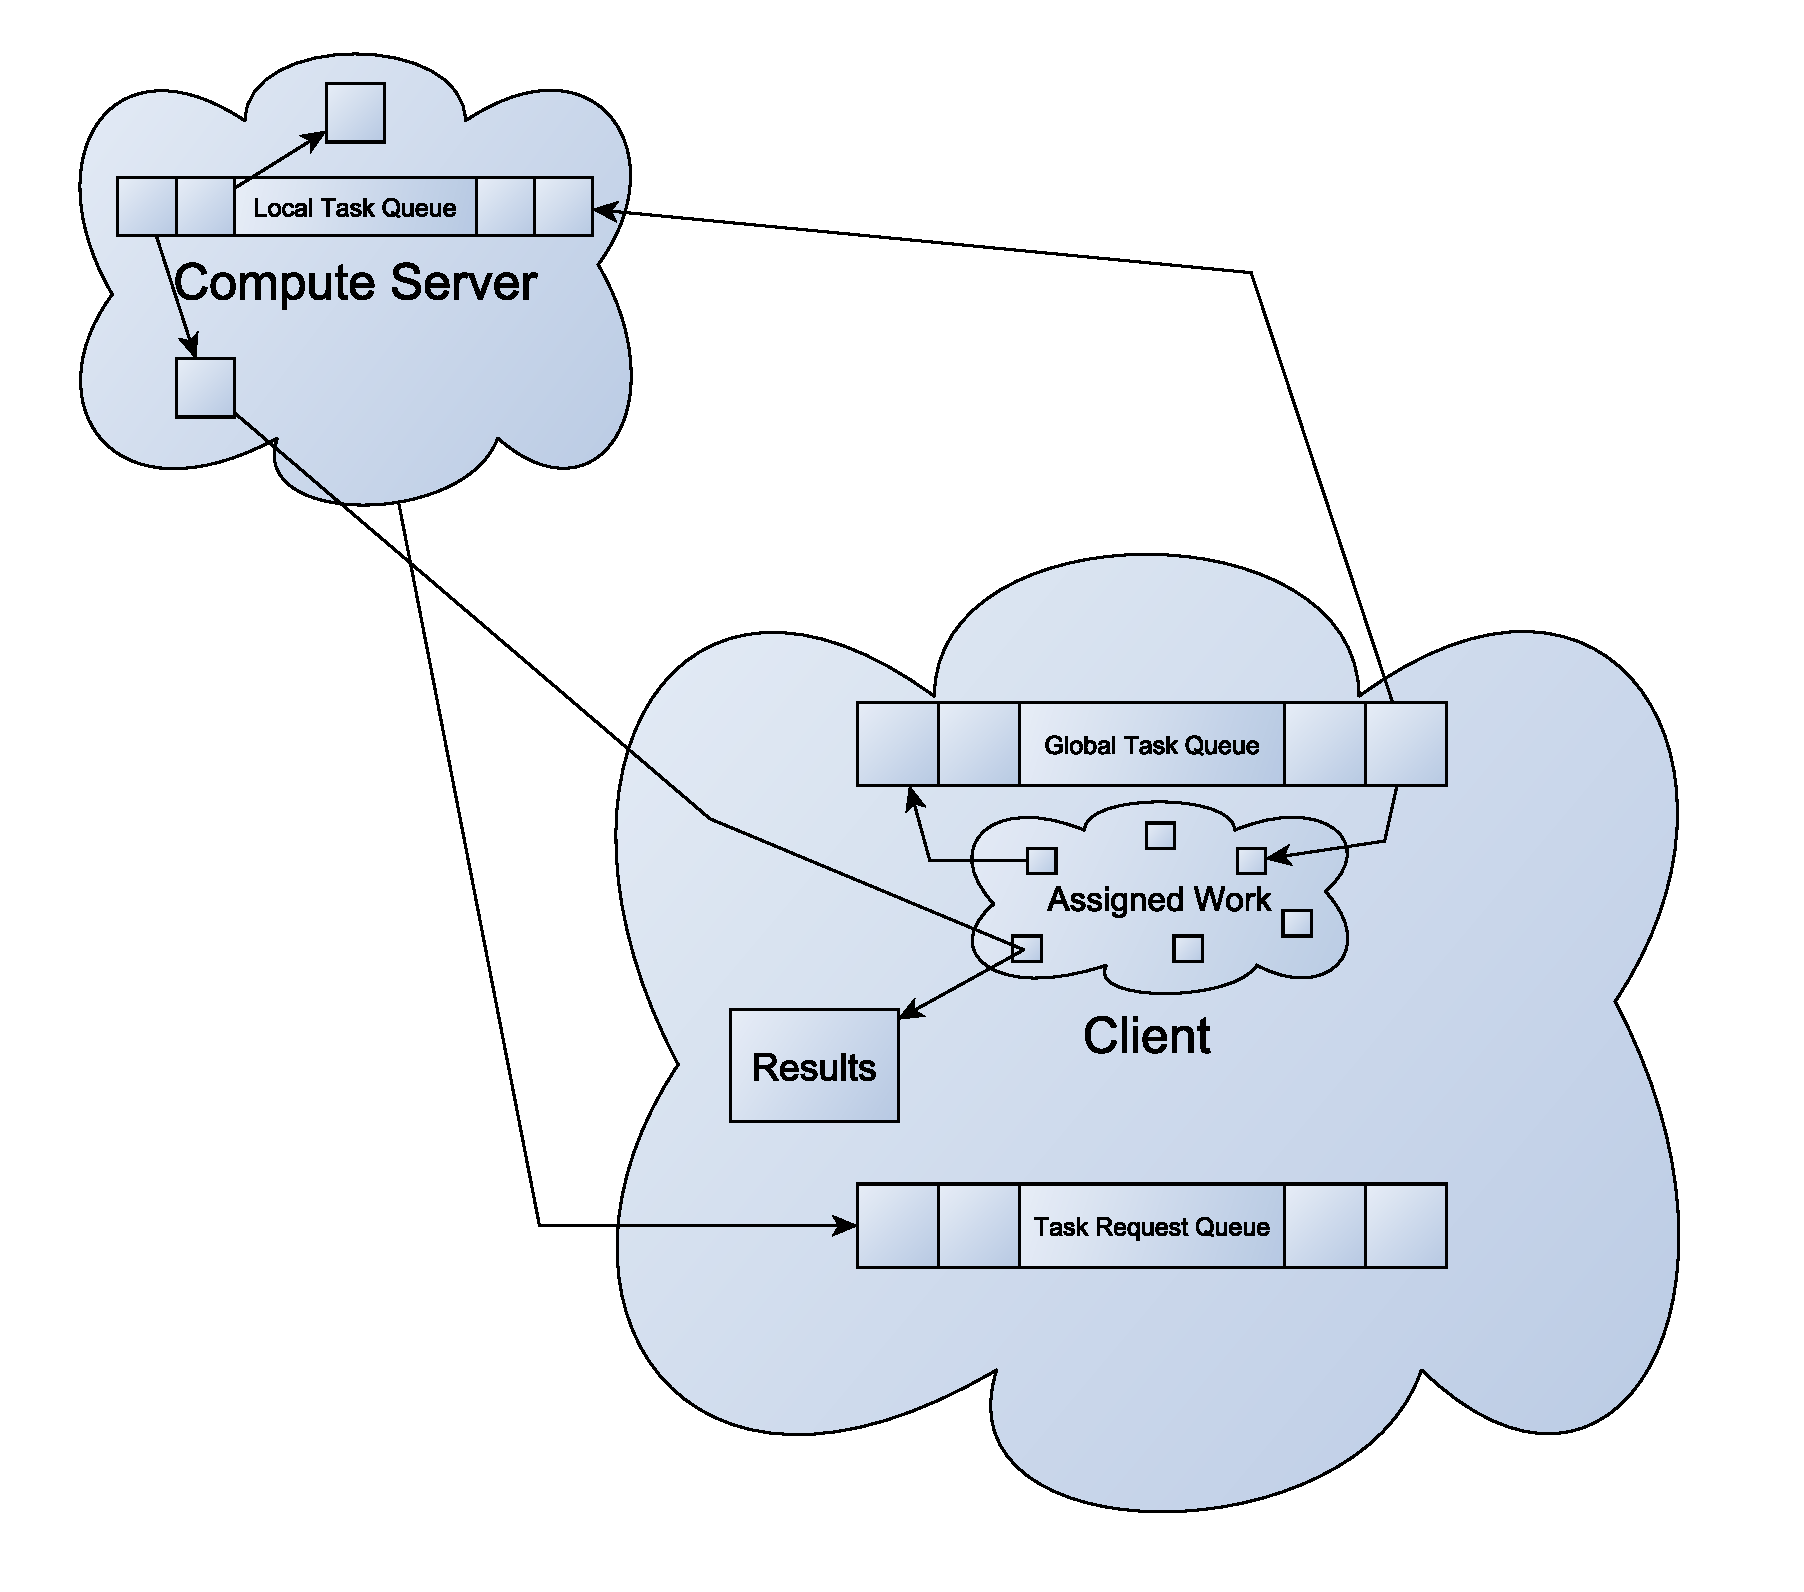
\includegraphics[width=4.5in, height=4.5in]{Images/FaultTolerant-Model.pdf}
	}
	\caption{Fault-Tolerant Model}
	\label{chapter:ft:model-figure}
\end{figure}

The purpose of the Assigned Work set is to have a way of identifying tasks that have been sent out for computation, but have not yet had their results returned. When a task is distributed to a compute server, that task is placed into the Assigned Work set, and given a maximum time in which a result is expected. In the normal case, when no failure has occurred, and when the task results are returned to the client, the task is removed from the Assigned Work set. In the failure case, the system periodically examines the Assigned Work set for any tasks that have not completed in their expected time and returns them to the Global Task Queue to match them with a new task request and sent back out for computation at a new compute server.

This change in the logic of the core client system to handle server failures, along with the existing ability to dynamically add new servers, is what allows the system to gracefully grow or shrink as computing resources come and go. With this model, we have now achieved the goal of a scalable, distributed, and fault-tolerant system. It is scalable in that it takes advantage of new computing resources, both CPU cores and distributed, is distributed, and can handle failures of connected servers.

I acknowledge the system has an important single point of failure at the client. If the client fails, the entire system fails. The solution to this is going to take a lot more work and is beyond the intended scope of this book. A future book is going to tackle this problem in a comprehensive manner.

\section{Framework Changes}\label{chapter:ft:section:framework-changes}

Based upon the new system model presented in Section \ref{chapter:ft:system-design}, various updates and additions to the core system framework have been implemented. In some places, such as the \texttt{Task} class, the changes are almost trivial, but in other places, such as the \texttt{TaskRequestQueue} the changes are more significant. Each of the core systems touched as part of adding fault-tolerance to the system is discussed in this section.

Before moving into the discussion of what is changed, it is useful to highlight the parts of the system that have seen no changes. Essentially everything about the server remains untouched. This includes the \texttt{ThreadPool}, the \texttt{TaskRequest}, and the \texttt{WorkerThread}. The entire networking infrastructure and message communication framework is untouched. The \texttt{Task} class is slightly modified, described in Section \ref{chapter:ft:section:task-update}, but not in a way that affects the server. Even though adding (server failure) fault-tolerance to the system is a big deal, the changes are actually localized to the client and do not impact the server.

\subsection{Updated \texttt{Task}}\label{chapter:ft:section:task-update}

\FigureGeneral \ref{chapter:ft:task-class} shows only the code associated with the updates to the \texttt{Task} class. A new \texttt{m\_duration} class member is added that represents the maximum amount of time it is expected for this task to be computed. The purpose of this duration is for failure detection. If the results for the task are not returned within this duration, a failure is detected and the task resubmitted to another server for computation. The constructor is updated to accept the duration parameter, with the expectation the derived classes set it to a value that is meaningful for the task. Finally, a new \texttt{getDuration} helper method is added to allow read-only access to the task duration.

\begin{code}[caption={Updated \texttt{Task} Class}, label=chapter:ft:task-class]
class Task
{
public:
  Task(std::chrono::milliseconds duration, Priority priority = Priority::One);

  std::chrono::milliseconds getDuration() const
  {
    return m_duration;
  }

private:
  std::chrono::milliseconds m_duration;
};
\end{code}

As a reminder, only the changed/added parts of the \texttt{Task} class are shown, all other parts of the class remain, but are not shown in the listing in order to help highlight the changes.

\subsection{New \texttt{AssignedTask}}\label{chapter:ft:section:assigned-task}

In order to identify which tasks have been distributed for computation, but have not yet returned a result, a new state (and container) is needed for tasks. The \texttt{AssignedTask} class is used as a wrapper around \texttt{Task} instances and held in a new container in the \texttt{TaskRequestQueue}. This wrapper contains a pointer to the original task, along with a deadline by which the result is expected before the task computation is considered to have failed. The declaration for the class is found in \FigureCode \ref{chapter:ft:assigned-task-class}.

\begin{code}[caption={\texttt{AssignedTask} Class}, label=chapter:ft:assigned-task-class]
class AssignedTask
{
public:
  explicit AssignedTask(std::shared_ptr<Tasks::Task> task);

  std::shared_ptr<Tasks::Task> getTask()
  {
    return m_task;
  }
  std::chrono::time_point<std::chrono::high_resolution_clock> 
    getDeadline() const 
    {
      return m_deadline;
    }

private:
  std::shared_ptr<Tasks::Task> m_task;
  std::chrono::time_point<std::chrono::high_resolution_clock> m_deadline;
};
\end{code}

When an instance of this class is created, the constructor, shown in \FigureCode \ref{chapter:ft:assigned-task-constructor}, takes the current time (\texttt{now}) and adds the task duration to it in order to come up with the deadline for when the task should have returned a result. This deadline is stored in the \texttt{m\_deadline} member of the class.

\begin{code}[caption={\texttt{AssignedTask} Constructor}, label=chapter:ft:assigned-task-constructor]
AssignedTask::AssignedTask(std::shared_ptr<Tasks::Task> task) :
  m_task(task)
{
  std::chrono::time_point<std::chrono::high_resolution_clock> now = 
    std::chrono::high_resolution_clock::now();
  m_deadline = now + task->getDuration();
}
\end{code}

When the \texttt{AssignedTask} instances are stored in a ordered container, a \texttt{std::priority\_queue} in our case, a means by which they can be sorted by their deadline is necessary. Therefore, the \texttt{AssignedTaskCompare} class shown in \FigureCode \ref{chapter:ft:assigned-task-compare} is necessary. This class overload the parenthesis \texttt{()} operator, taking two \texttt{AssignedTask} instances and returning a \texttt{true/false} depending upon which one is greater than the other. When the \texttt{std::priority\_queue} is declared in the \texttt{TaskRequestQueue}, this class is specified as the comparison functor. Using this scheme makes it possible to easily know which tasks have gone past their deadline; how this is done is discussed in futher detail in Section \ref{chapter:ft:section:task-request-queue}, which details the updated \texttt{TaskRequestQueue}.

\begin{code}[caption={\texttt{AssignedTaskCompare} Class}, label=chapter:ft:assigned-task-compare]
class AssignedTaskCompare : 
  public std::binary_function<
    std::shared_ptr<AssignedTask>,
    std::shared_ptr<AssignedTask>, bool>
{
public:
  bool operator()(
    const std::shared_ptr<AssignedTask> lhs, 
    const std::shared_ptr<AssignedTask> rhs) const
  {
    return (lhs->getDeadline() > rhs->getDeadline());
  }
};
\end{code}

\subsection{Updated \texttt{TaskRequestQueue}}\label{chapter:ft:section:task-request-queue}

The most significant changes to the code take place in the \texttt{TaskRequestQueue} class. \FigureCode \ref{chapter:ft:task-request-queue} shows the additions to the class; everything else presented in Chapter \ref{chapter:dist} remains part of the class, however with some of the method implementations changed. As noted before, the server code is essentially unchanged. It is the client code where the fault-tolerance logic was added, resulting in the large changes to the \texttt{TaskRequestQueue} class. Each of these additions, and changes to existing methods, is detailed next.

\begin{code}[caption={Updated \texttt{TaskRequestQueue}}, label=chapter:ft:task-request-queue]
class TaskRequestQueue
{
public:
  bool finalizeTask(uint32_t id, bool forceRemove);

private:
  std::priority_queue<
    std::shared_ptr<AssignedTask>,
    std::vector<std::shared_ptr<AssignedTask>>, 
    AssignedTaskCompare> m_queueAssigned;
  std::unordered_map<uint32_t, std::shared_ptr<AssignedTask>> m_mapAssigned;
  std::recursive_mutex m_mutexAssigned;

  void compactQueueAssigned();
  bool isQueueAssignedEmpty();
  void popQueueAssigned();
  bool mapAssignedContains(uint32_t id);
  boost::optional<std::shared_ptr<AssignedTask>> getQueueAssignedTop();
};
\end{code}

Let's start by looking at the updated \texttt{distribute} method in \FigureCode \ref{chapter:ft:distribute}. While looking at the revised \texttt{distribute} method, refer back to Chapter \ref{chapter:dist} and \FigureCode \ref{chapter:dist:trq:distribute} for the orginal implemention to get a better sense of the scope of the changed logic.

\begin{code}[caption={Updated \texttt{distribute} Method}, label=chapter:ft:distribute]
while (!m_distributerDone)
{
  Tasks::Task::Priority currentPriority = m_priority;
  bool donePriority = false;
  while (!m_distributerDone && !donePriority)
  {
    bool distributed = false;
    std::shared_ptr<Tasks::Task> task;

    compactQueueAssigned();

    if (!isQueueAssignedEmpty())
    {
      auto top = getQueueAssignedTop();
      if (top)
      {
        std::chrono::time_point<std::chrono::high_resolution_clock> now = 
          std::chrono::high_resolution_clock::now();
        if (top.get()->getDeadline() <= now)
        {
          task = top.get()->getTask();
          popQueueAssigned();
          finalizeTask(task->getId(), true);

          fillRequest(task);
          distributed = true;
        }
      }
    }
    if (!distributed)
    {
      task = m_queueTasks.dequeue(currentPriority);
      if (task)
      {
        fillRequest(task.get());
        distributed = true;
      }
    }
    Tasks::updatePriority(
      distributed, 
      m_priority, 
      donePriority, 
      currentPriority);
  }
  if (!m_distributerDone)
  {
    std::unique_lock<std::mutex> lock(m_mutexEventTask);
    m_eventTask.wait_for(
      lock, 
      std::chrono::milliseconds(100));
  }
}
\end{code}

The code uses the same logic to stay in the method, waiting for the \texttt{m\_distributerDone} flag to change to \texttt{true}. The fault-tolerant design retains the same priority scheduling algorithm as before, therefore, the same steps and priority loop are used. At this point, the same fundamental loop to keep distributing tasks and working downward through priority is intact. The changes to the method begin inside the priority loop.

The first change is a call to the \texttt{compactQueueAssigned} method, which removes items from the assigned queue that have returned results since the last time this loop was executed (all new methods refered to in this section are further detailed below). The next step in the logic is to look at the assigned queue to see if it contains anything (the items in this queue are sorted by their deadline). If it does, the top (i.e. the oldest) item's deadline is examined to see if it is past the current time. If it is, it is removed from the assigned queue (\texttt{popQueueAssigned}), the task is finalized (\texttt{finalizeTask}), then the task is used to fill the next available request. If the assigned queue does not contain anything, a task is dequeued from the main task queue (\texttt{m\_queueTasks}) and that is used to fill the next available request.

One additional change is made at the bottom of the loop inside the \texttt{if (!m\_distributerDone)} condition. Rather than doing an indefinite \texttt{.wait} on the condition variable a \texttt{.wait\_for} is used instead. This is done because it is possible for there to be a single task being computed, and no other tasks waiting to be distributed, and then a failure occurs. The \texttt{.wait\_for} allows the loop to periodically wake up and check the assigned queue for tasks that have gone past their deadline and attempt to fill them on another server.

The next piece of code to take a look at is the revised \texttt{fillRequest} method. The core logic is the same as from Chapter \ref{chapter:dist}, but a few important additions have been made. \FigureCode \ref{chapter:ft:fill-request} shows the updated sections of this method; for reference, the original method from the previous chapter is located at \FigureCode \ref{chapter:dist:trq:fill-request}. The first new addition happens at the beginning with a call to the \texttt{removeDisconnected} method of the \texttt{m\_servers} member. The purpose of this is to detect servers that are no longer connected (i.e. have failed) and remove them from consideration for filling task assignments.

\begin{code}[caption={Revised \texttt{fillRequest} Method}, label=chapter:ft:fill-request]
void TaskRequestQueue::fillRequest(std::shared_ptr<Tasks::Task> task)
{
  m_servers->removeDisconnected();

  ...

  m_ioService->post(
    [this, serverId, task]()
    {
      {
        std::lock_guard<std::recursive_mutex> lock(m_mutexAssigned);
        std::shared_ptr<AssignedTask> 
          assigned = std::make_shared<AssignedTask>(task);
        m_queueAssigned.push(assigned);
        m_mapAssigned[task->getId()] = assigned;
      }

      task->send(
        m_servers->get(serverId)->socket, 
        *m_servers->get(serverId)->strand);
    });
}
\end{code}

The next revision to the \texttt{fillRequest} method is in the post to the \texttt{io\_service}. In the previous implementation it was enough to send the task to the selected server and forget about it. Now, with the desire to handle server failures, it is necessary to track the task. This is done through the addition of two new data structures to the \texttt{TaskRequestQueue}. The first is a \texttt{priority\_queue} of \texttt{AssignedTask}s, with priority determined by the deadline of the task. The second is an \texttt{unordered\_map} of \texttt{AssignedTask}s.

Why two different data structures to hold the same information? Performance! The \texttt{priority\_queue} is used during the \texttt{distribute} method to find out if there are any tasks past their deadline. A \texttt{priority\_queue} is the most efficient data structure to do this, only the top of the queue needs to be examined. The \texttt{unordered\_map}, on the other hand, is used to keep track of which tasks have been assigned, but results not yet returned. When the \texttt{compactQueueAssigned} method is invoked during the \texttt{distribute} loop, the \texttt{m\_mapAssigned} is used to know which items should be removed from the top of the \texttt{m\_queueAssigned} queue. By using a hash table for the \texttt{m\_mapAssigned}, once again, the best possible performance is achieved. The code in \FigureCode \ref{chapter:ft:compact-queue} shows this process taking place.

\begin{code}[caption={Compacting The Assigned Queue}, label=chapter:ft:compact-queue]
void TaskRequestQueue::compactQueueAssigned()
{
  std::lock_guard<std::recursive_mutex> lock(m_mutexAssigned);

  bool done = false;
  while (!isQueueAssignedEmpty() && !done)
  {
    auto top = getQueueAssignedTop();
    if (top)
    {
      if (!mapAssignedContains(top.get()->getTask()->getId()))
      {
        popQueueAssigned();
      }
      else
      {
        done = true;
      }
    }
  }
}
\end{code}

The \texttt{removeDisconnected} method deserves a discussion. The purpose of the method is to go through the set of currently known servers and remove any that are no longer connected. The code for the method is shown in \FigureCode \ref{chapter:ft:remove-disconnected}. As with the others, this method is synchronized on the instance mutex to ensure no other code is accessing the \texttt{m\_servers} member during its operation.

\begin{code}[caption={Remove Disconnected Servers}, label=chapter:ft:remove-disconnected]
void ServerSet::removeDisconnected()
{
  std::lock_guard<std::mutex> lock(m_mutex);

  std::vector<ServerID_t> removeMe;
  for (auto server : m_servers)
  {
    if (!server.second.socket->is_open())
    {
      removeMe.push_back(server.first);
    }
  }
  for (auto server : removeMe)
  {
    m_servers.erase(server);
  }
}
\end{code}

A two-step process is used to discover disconnected servers and then remove them from the hash table. The first is to iterate over the set of servers and check to see if their socket connection is still open. If it is no longer open, the \texttt{id} (the \texttt{first} member of the \texttt{std::pair}) of the server is added to the \texttt{removeMe} vector. Following this, the servers identified in the first step are removed from the \texttt{m\_servers} hash table.

When the results for a task are received, the task needs to be removed from tracking so that it isn't considered for resubmission to another server when its deadline passes. To do this, application code must call into the \texttt{finalizeTask} of the \texttt{TaskRequestQueue}, the code for this method is shown in \FigureCode \ref{chapter:ft:finalize-task}.

\begin{code}[caption={Finalizing A Task}, label=chapter:ft:finalize-task]
bool TaskRequestQueue::finalizeTask(uint32_t id, bool forceRemove)
{
  bool removed = false;

  std::lock_guard<std::recursive_mutex> lock(m_mutexAssigned);

  auto it = m_mapAssigned.find(id);
  if (it != m_mapAssigned.end())
  {
    std::chrono::time_point<std::chrono::high_resolution_clock> 
      now = std::chrono::high_resolution_clock::now();
    if (it->second->getDeadline() >= now  || forceRemove)
    {
      m_mapAssigned.erase(it);
      removed = true;
    }
  }

  return removed;
}
\end{code}

The first step in this method is to check to see if the task exists in the tracking hash table, \texttt{m\_mapAssigned}. If it doesn't, nothing is done and \texttt{false} is returned. If it is found, the deadline is checked to see if it is in the future. If the deadline is in the future (or the \texttt{forceRemove} flag is set), then the task is removed from tracking. On the other hand, if the deadline has passed, it isn't removed. The reason for leaving a task past its deadline in the hash table is to have the function return \texttt{false}, indicating to the application code the results for this task should be ignored. This can happen when the system gets too far behind in computing results and re-sends a task out for comptuation even when no server failures have occurred. The fixed estimate for how long a computation should take has its limitations. The next book in this series will solve that problem.

\section{Application Changes}\label{chapter:ft:section:app-changes}

Because fault-tolerance is applied at the core system level, changes to the application code are essentially trivial. The only change to the application code is to make use of a new method on the \texttt{TaskRequestQueue}, a call to the \texttt{finalizeTask} method described earlier in Section \ref{chapter:ft:section:task-request-queue}. Whenever a result is received by the application code, the task associated with the result needs to be finalized.

The code in \FigureCode \ref{chapter:ft:app:finalize-task} demonstrates the use of the \texttt{finalizeTask} method. As described in Chapter \ref{chapter:dist}, reading of the result message is performed first. But now, before the result is processed by application specific code, the task associated with the result must be finalized. If the \texttt{finalizeTask} method returns \texttt{true} the result may be used, otherwise it must be ignored (likely because it is a duplicate from a resubmitted task).

\begin{code}[caption={Use of \texttt{finalizeTask}}, label=chapter:ft:app:finalize-task]
void FaultTolerantApp::processMandelResult(
  ServerID_t serverId)
{
  Messages::MandelResultMessage taskResult;
  taskResult.read(m_servers.get(serverId)->socket);

  if (TaskRequestQueue::instance()->finalizeTask(taskResult.getTaskId()))
  {
    m_mandelbrot->processMandelResult(taskResult);
  }
}
\end{code}

That is it, no other changes to the application code are necessary!

	% Copyright � 2015 by James Dean Mathias
% All Rights Reserved

\chapter{Scalability - Fault-Tolerant - Task Dependencies}\label{chapter:ftdag}

The final evolution of the code in this book is to return to the topic of Chapter \ref{chapter:scalable-dag} and incorporate the ability to have the executation of a task, or tasks, depend upon the completion of another task, or tasks, within the context of the distributed and fault-tolerant system. With this final step, we end up with a powerful system, one that exceeds the original goal of the book: a scalable, distributed, and fault-tolerant system, with the added sophistication of being able to handle arbitrary dependency complexity among tasks.

The heavy lifting for the task dependency work was done back in Chapter \ref{chapter:scalable-dag} with the introduction and integration of the \texttt{ConcurrentDAG}. As a result, this chapter is fairly light, focusing only on the changes necessary to migrate the fault-tolerant code from Chapter \ref{chapter:ft} to make use of the \texttt{ConcurrentDAG} to ensure task dependecies are supported.

\section{Framework Changes}\label{chapter:ftdag:section:framework-changes}

The core framework is changed in three fairly minor ways. The first is the complete removal of the concept of priority. While it is possible to have the concept of priority with task dependencies, that is not a topic covered by this book. The next change is to use the \texttt{ConcurrentDAG} in place of the \texttt{ConcurrentMultiqueue}. The final change is an update to the \texttt{finalizeTask} method of the \texttt{TaskRequestQueue}.

As just noted, the \texttt{m\_queueTasks} is changed from a \texttt{ConcurrentMultiqueue} to the \texttt{ConcurrentDAG} first introduced in Chapter \ref{chapter:scalable-dag}. Making this change does result in some other code changes because its interface is different. For example, the \texttt{ConcurrentDAG} has the concepts of adding a node (a single task) or an edge (dependent tasks), whereas the \texttt{ConcurrentMultiqueue} only has the concept of adding tasks (a node in the \texttt{ConcurrentDAG}). Additionally, the \texttt{enqueueTask} method that allows dependent tasks to be defined is added to the \texttt{TaskRquestQueue}, providing a way to add tasks with dependencies between them.

In addition to using the \texttt{ConcurrentDAG}, there is one small change in the code from Chapter \ref{chapter:scalable-dag}; this is the same change as was done to the \texttt{ConcurrentPriorityQueue} as discussed in Section \ref{chapter:dist:section:concurrent-priorityqueue} of Chapter \ref{chapter:dist}. The return type for the \texttt{dequeue} operation is now a \texttt{boost::optional}. Again, now that the \texttt{boost} library is a part of the project, it makes sense to change this return type.

The change to the \texttt{finalizeTask} method is worth a closer look; \FigureCode \ref{chapter:ftdag:code:finalize-task} shows the updated code. The first new item is the addition of the \texttt{dagRemove} parameter. When this parameter is set to \texttt{true}, the task is removed from the DAG (\texttt{m\_queueTasks}) allowing its dependent tasks to be released for computation. The reason for not removing the task from the DAG is for fault-tolerance. In the case of a server failure it is desired the task remains in the DAG to ensure its dependent tasks are not yet released. The final change is at the bottom of the function, a \texttt{.notify\_all} call is made on the condition variable \texttt{m\_eventTask} to allow the distributor to immediately look at any tasks that may have been released for computation.

\begin{code}[caption={Updated \texttt{finalizeTask}}, label=chapter:ftdag:code:finalize-task]
bool TaskRequestQueue::finalizeTask(
  uint32_t id,
  bool dagRemove,
  bool forceRemove)
{
  std::lock_guard<std::recursive_mutex> lock(m_mutexAssigned);
  bool removed = false;

  auto it = m_mapAssigned.find(id);
  if (it != m_mapAssigned.end())
  {
    if (dagRemove)
    {
      m_queueTasks.finalize(it->second->getTask());
    }

    std::chrono::time_point<std::chrono::high_resolution_clock> 
      now = std::chrono::high_resolution_clock::now();
    if (it->second->getDeadline() >= now || forceRemove)
    {
      m_mapAssigned.erase(it);
      removed = true;
    }
  }

  m_eventTask.notify_all();
  return removed;
}
\end{code}

That is all, the changes to the framework are quite modest. This is due to a reasonable (admittedly not perfect) design that abstracts different layers of the system from each other. In particular, this allows a near drop-in replacement of going from a priority queue like data structure with a DAG data structure for the ordering of tasks for computation.

\section{Application Interface}

There are two ways in which tasks are added to the updated framework. The first is to add tasks and have them computed in the order they were placed on the \texttt{TaskRequestQueue}. This is as simple as creating the task, same as the previous two chapters (minus priority), and calling \texttt{enqueueTask} on the \texttt{TaskRequestQueue}. The second way is to add tasks but define a dependency relationship between them. This is the same concept introduced in Chapter \ref{chapter:scalable-dag}. Nothing new here from the application interface. The big change, and transparent to the application code, is that the tasks are distributed among as many compute servers as are connected, in addition to being fault-tolerant.

With all of the above in place, the application interface to the \texttt{TaskRequestQueue} includes the members shown in \FigureCode \ref{chapter:ftdag:code:trq-interface}:

\begin{code}[caption={\texttt{TaskRequestQueue} Interface}, label=chapter:ftdag:code:trq-interface]
void beginGroup();
void endGroup();
void enqueueTask(std::shared_ptr<Tasks::Task> source);
void enqueueTask(
  std::shared_ptr<Tasks::Task> source,
  std::shared_ptr<Tasks::Task> dependent);
bool finalizeTask(
  uint32_t id,
  bool dagRemove,
  bool forceRemove);
\end{code}

To add a task with no dependencies, only the \texttt{enqueueTask} method is called. When the task is complete (i.e. results returned), the \texttt{finalizeTask} method must be called.

To define dependencies among tasks, all tasks that have dependency relationships must be added as a group. The first step is to call \texttt{beginGroup}, followed by using the overloaded \texttt{enqueueTask} method that allows two tasks to be added; where the second task cannot be computed until the first task is completed. Once all tasks are added and \texttt{endGroup} is called, which allows the scheduling to begin selecting tasks and distributing them for computation. The next two sections of this chapter, Section \ref{chapter:ftdag:demo:mandelbrot} and Section \ref{chapter:ftdag:demo:complex} show detailed examples of using the interface to add tasks with dependencies.

\section{Mandelbrot Changes}\label{chapter:ftdag:demo:mandelbrot}

In Chapters \ref{chapter:dist} and \ref{chapter:ft} the \texttt{Mandelbrot} class used a couple of member variables, \texttt{m\_tasksSent} and \texttt{m\_tasksReceived}, to track when all the results for a single Mandelbrot image were complete and available for display. This works well enough, but I thought it would be interesting to show another way to achieve this same functionality through the use of task dependencies, letting the system framework help track when an image is complete. I am not necessarily recommending this is a better approach (in fact it can be argued it is somewhat less performant because of the networking time involved) but merely making this change to show how task dependencies work.

The first change is to create a new task type, it is called \texttt{MandelFinishedTask}; the class declaration for this task is shown in \FigureCode \ref{chapter:ftdag:code:mandel-finished-task}. This task has no actual computation associated with it, instead, it is used as a way for the application code to send a message to itself when all other Mandelbrot tasks are complete. In other words, its \textit{execution} is dependent upon the completion of all \texttt{MandelTask} executions.

\begin{code}[caption={\texttt{MandelFinishedTask} Class}, label=chapter:ftdag:code:mandel-finished-task]
class MandelFinishedTask : public Task
{
public:
  MandelFinishedTask() :
    Task(std::chrono::milliseconds(1000))
  {
  }

  MandelFinishedTask(
    std::shared_ptr<ip::tcp::socket> socket,
    Messages::MandelFinishedMessage& message) :
    Task(socket, message.getTaskId())
  {
  }

  virtual void execute() override;

protected:
  virtual std::shared_ptr<Messages::Message> getMessage() override;
  virtual std::shared_ptr<Messages::Message> 
    completeCustom(boost::asio::io_service& ioService) override;
};
\end{code}

With the new \texttt{MandelFinishedTask} available as a kind of application signal, it can be used in combination with the existing \texttt{MandelTask} task to inform the application code when the full Mandelbrot image is available. Take a look at the updated \texttt{startNewImage} method in \FigureCode \ref{chapter:ftdag:code:start-new-image} to see how the task dependencies are defined.

\begin{code}[caption={Generation Mandelbrot Tasks}, label=chapter:ftdag:code:start-new-image]
void Mandelbrot::startNewImage()
{
  TaskRequestQueue::instance()->beginGroup();

  auto taskFinished = std::make_shared<Tasks::MandelFinishedTask>();

  double deltaX = (m_mandelRight - m_mandelLeft) / m_sizeX;
  double deltaY = (m_mandelBottom - m_mandelTop) / m_sizeY;
	
  for (auto row : IRange<uint16_t>(0, m_sizeY - 1, MANDEL_COMPUTE_ROWS))
  {
    auto task = std::make_shared<Tasks::MandelTask>(
        row, 
        std::min(row + MANDEL_COMPUTE_ROWS - 1, m_sizeY - 1), 
        m_sizeX, m_mandelLeft, m_mandelTop + row * deltaY, 
        deltaX, deltaY, 
        MANDLE_MAX_ITERATIONS);
    TaskRequestQueue::instance()->enqueueTask(
      task, 
      taskFinished);
  }

  TaskRequestQueue::instance()->endGroup();
}
\end{code}

The first step in this method is to call \texttt{beginGroup} to ensure all of the Mandelbrot tasks are added before any are considered for scheduling. The second step is to create the \texttt{MandelFinishedTask} so that it can be identified in the \texttt{enqueueTask} calls as a dependent. The third step is to define \texttt{taskFinished} as being dependent upon every other \texttt{MandelTask} computation before it can be sent out for \textit{execution}. Finally, the \texttt{endGroup} method is called on the \texttt{TaskRequestQueue} which releases all of these tasks for computation.

In the \texttt{FaultTolerantApp} class, a new \texttt{processMandelFinishedResult} handler is defined for the \texttt{MandelFinishedTask}, shown in \FigureCode \ref{chapter:ftdag:code:mandel-finished-handler}. When the \texttt{MandelFinishedTask} result is sent back to the client this handler is inovked, and this handler is guaranteed to only be invoked after all other \texttt{MandelTask} results have been sent back because it is dependent upon all of those tasks first having been executed. At this point, it is known the full new Mandelbrot image is returned and a new one can be generated.

\begin{code}[caption={\texttt{MandelFinishedTask} Handler}, label=chapter:ftdag:code:mandel-finished-handler]
void FaultTolerantApp::processMandelFinishedResult(
  ServerID_t serverId)
{
  Messages::MandelFinishedResultMessage taskResult;
  taskResult.read(m_servers.get(serverId)->socket);

  if (TaskRequestQueue::instance()->finalizeTask(
    taskResult.getTaskId(), true, true))
  {
    m_mandelbrot->processMandelFinishedResult(taskResult);
  }
}
\end{code}

The code for this handler follows the familiar pattern already established in the previous chapter. First step is to finish reading the message, the next step is to finalize the task, and the final step is to do something application specific based upon the result. In this case, the application specific code is to call back into the \texttt{Mandelbrot} class to let it know the full image is complete. At this point, the \texttt{Mandelbrot} code sets the \texttt{m\_inUpdate} flag to \texttt{false}, which allows another set of Mandelbrot computation tasks to be generated when necessary.

Having this new task added removes the need for the member variables in the \texttt{Mandelbrot} class to track how many tasks were sent, received, and constantly checking them to see if the correct number have been returned. Instead, that accounting is implicit information contained in the graph representation of the Mandelbrot tasks. When the \texttt{MandelFinishedTask} result shows up, that is the signal the full image is complete, no other accounting is necessary.

\section{Complex Demonstration}\label{chapter:ftdag:demo:complex}

This section provides an example that hints at the kind of complexity supported by this framework, it demonstrates the creation of a non-trivial task dependency graph. The diagram in \FigureGeneral \ref{chapter:ftdag:figure:demonstration} shows a graph of tasks and their dependencies. The tasks at the top of the graph (8 through 15) have no dependencies and therefore, can be computed in any order. The second level of tasks (4 through 7) have dependencies on the first level of tasks, this continues through the third level. Next, task 1 shows dependencies on tasks 2 and 3, which have cascading dependencies on all other tasks, meaning that task 1 can only be computed after all other tasks above it in the graph have completed their execution. Once task 1 has completed its execution, tasks 16 and 17 can compute in parallel, and this continues until the last row of tasks (22 through 29) are free from dependencies and can compute in parallel.

%
% Good tkz-graph reference: http://mirror.hmc.edu/ctan/macros/latex/contrib/tkz/tkz-graph/doc/tkz-graph-screen.pdf
%
\begin{figure}[width=4.5in, height=4.5in]
	\centering
		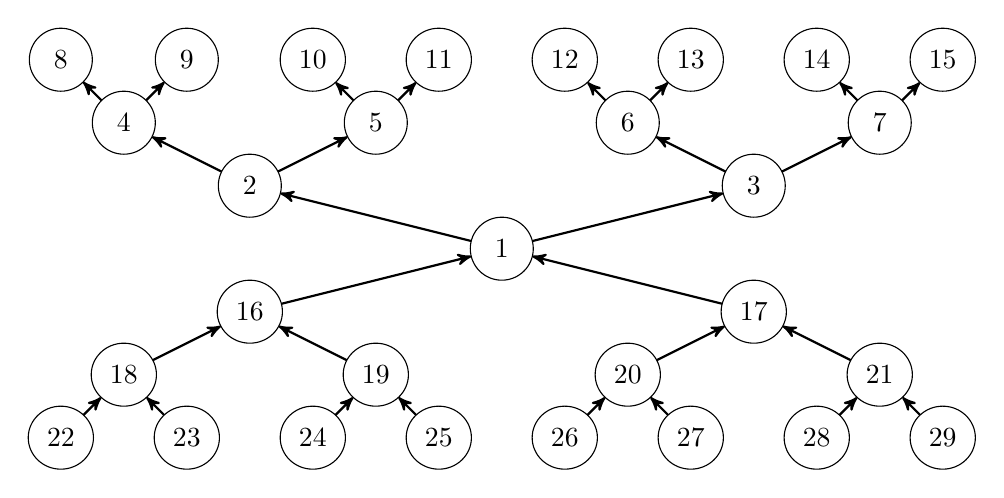
\begin{tikzpicture}[scale=0.8]
			\tikzstyle{VertexStyle} = [shape = ellipse, minimum size = 8mm, draw]
			\tikzstyle{EdgeStyle}   = [->,>=stealth']
			\SetGraphUnit{2}
			%\draw[help lines] (0,0) grid (14,7);
			\Vertex[x=7, y=3]{1}
			\Vertex[x=3, y=4]{2} \Vertex[x=11, y=4]{3}
			\Vertex[x=1, y=5]{4} \Vertex[x=5, y=5]{5} \Vertex[x=9, y=5]{6} \Vertex[x=13, y=5]{7}
			\Vertex[x=0, y=6]{8} \Vertex[x=2, y=6]{9} \Vertex[x=4, y=6]{10} \Vertex[x=6, y=6]{11}
			\Vertex[x=8, y=6]{12} \Vertex[x=10, y=6]{13} \Vertex[x=12, y=6]{14} \Vertex[x=14, y=6]{15}
			
			\Edges(1,3,7,15) \Edges(3,6,13) \Edges(6,12) \Edges(7,14)
			\Edges(1,2,4,8) \Edges(2,5,11) \Edges(5,10) \Edges(4,9)
			
			\Vertex[x=3, y=2]{16} \Vertex[x=11, y=2]{17}
			\Vertex[x=1, y=1]{18} \Vertex[x=5, y=1]{19} \Vertex[x=9, y=1]{20} \Vertex[x=13, y=1]{21}
			\Vertex[x=0, y=0]{22} \Vertex[x=2, y=0]{23} \Vertex[x=4, y=0]{24} \Vertex[x=6, y=0]{25}
			\Vertex[x=8, y=0]{26} \Vertex[x=10, y=0]{27} \Vertex[x=12, y=0]{28} \Vertex[x=14, y=0]{29}
			
			\Edges(22,18,16,1) \Edges(24,19,16) \Edges(23,18) \Edges(25,19)
			\Edges(29,21,17,1) \Edges(27,20,17) \Edges(26,20) \Edges(28,21)
			
		\end{tikzpicture}
	\caption{Complex DAG}\label{chapter:ftdag:figure:demonstration}
\end{figure}

%
% tikz references:
%    http://www.texample.net/
%    http://sourceforge.net/projects/pgf/
%    http://www.bu.edu/math/files/2013/08/tikzpgfmanual.pdf

%\begin{figure}
%	\centering
%		\begin{tikzpicture}
%			\tikzstyle{edge from parent}=[->, >=stealth', thick, draw]
%			\tikzstyle{every node}=[circle, draw, minimum size=8mm]
%			\tikzstyle{level 1}=[sibling distance=60mm]
%			\tikzstyle{level 2}=[sibling distance=30mm]
%			\tikzstyle{level 3}=[sibling distance=15mm]
%			\tikzstyle{level 4}=[sibling distance=8mm]
%			\node (v1) {1} [grow=up]
%				child {node {2}
%					child {node {4}
%						child {node {8}}
%						child {node {9}}
%					}
%					child {node {5}
%						child {node {10}}
%						child {node {11}}
%					}
%				}
%				child {node {3}
%					child {node {6}
%						child {node {12}}
%						child {node {13}}
%					}
%					child {node {7}
%						child {node {14}}
%						child {node {15}}
%					}
%				};
%		\end{tikzpicture}
%	\caption{Tree DAG}\label{chapter:ftdag:task-tree-figure}
%\end{figure}

The code involved in creating this task graph is relatively straightforward, following the pattern we know by now. The first step involved writing a new task class for the demonstration. The next step was to create the two messages used to send the task to a compute server and return the results back to the client. Finally, some application code was written to define the relationships among the tasks.

The task class for this demonstration is named \texttt{DAGExampleTask}, its class declaration is found in \FigureCode \ref{chapter:ftdag:code:dag-example-task}. This code should be quite familiar by now. The only items of note are the \texttt{name} constructor parameter and the private data member \texttt{m\_name}. When an instance of this task is created, it is given a \texttt{std::string} name that is sent to the compute server and returned as part of the result, allowing the application to report to the console the name of the task results just received.

\begin{code}[caption={\texttt{DAGExampleTask} Class}, label=chapter:ftdag:code:dag-example-task]
class DAGExampleTask : public Task
{
public:
  DAGExampleTask(std::string name) :
  Task(std::chrono::milliseconds(5000)),
    m_name(name)
  {
  }

  DAGExampleTask(std::shared_ptr<ip::tcp::socket> 
    socket,
    Messages::DAGExampleMessage& message) :
    Task(socket, message.getTaskId()),
    m_name(message.m_name)
  {
  }

  virtual void execute() override;

protected:
  virtual std::shared_ptr<Messages::Message> getMessage() override;
  virtual std::shared_ptr<Messages::Message> 
    completeCustom(boost::asio::io_service& ioService) override;

private:
  std::string m_name;
};
\end{code}

The \texttt{DAGExampleTask} doesn't perform any real computation, instead it sleeps for 4 seconds, as shown in \FigureCode \ref{chapter:ftdag:code:dag-example-execute}. The reason for having the execution sleep for this amount of time is to give time for one to progressively watch the results returned and displayed to the console. Note back in \FigureCode \ref{chapter:ftdag:code:dag-example-task} this \texttt{DAGExampleTask} constructor is defined to have a fault-tolerant timeout of 5 seconds (5000 milliseconds), 1 second longer than the execution. For any reason, if you change the execution sleep period, make sure to adjust the fault-tolerant timeout to be longer than the sleep.

\begin{code}[caption={\texttt{DAGExampleTask} Execution}, label=chapter:ftdag:code:dag-example-execute]
void DAGExampleTask::execute()
{
  std::this_thread::sleep_for(std::chrono::milliseconds(4000));
}
\end{code}

Once the results for a \texttt{DAGExampleTask} are returned to the client, the \texttt{processDAGExampleResult} method is invoked, as shown in \FigureCode \ref{chapter:ftdag:code:results-handler}. The only thing the handler does is to report the name of the task to the console.

\begin{code}[caption={\texttt{DAGExampleTask} Results Handler}, label=chapter:ftdag:code:results-handler]
void FaultTolerantApp::processDAGExampleResult(
  ServerID_t serverId)
{
  Messages::DAGExampleResultMessage taskResult;
  taskResult.read(m_servers.get(serverId)->socket);

  if (TaskRequestQueue::instance()->finalizeTask(
    taskResult.getTaskId(), true, true))
  {
    std::cout << "DAG Example Task: " << taskResult.getName() << std::endl;
  }
}
\end{code}

The big question is, with such a simple interface for adding tasks, how can such a complex dependency graph as shown in \FigureGeneral \ref{chapter:ftdag:figure:demonstration} get defined. It turns out to be quite easy, refer to the code in \FigureCode \ref{chapter:ftdag:code:adding-tasks} to see how it is done.

\begin{code}[caption={Defining Task Dependencies}, label=chapter:ftdag:code:adding-tasks]
TaskRequestQueue::instance()->beginGroup();

auto task1 = std::make_shared<Tasks::DAGExampleTask>("1");
auto task2 = std::make_shared<Tasks::DAGExampleTask>("2");
auto task3 = std::make_shared<Tasks::DAGExampleTask>("3");
auto task4 = std::make_shared<Tasks::DAGExampleTask>("4");
auto task5 = std::make_shared<Tasks::DAGExampleTask>("5");
auto task6 = std::make_shared<Tasks::DAGExampleTask>("6");
auto task7 = std::make_shared<Tasks::DAGExampleTask>("7");
auto task8 = std::make_shared<Tasks::DAGExampleTask>("8");
auto task9 = std::make_shared<Tasks::DAGExampleTask>("9");
auto task10 = std::make_shared<Tasks::DAGExampleTask>("10");
auto task11 = std::make_shared<Tasks::DAGExampleTask>("11");
auto task12 = std::make_shared<Tasks::DAGExampleTask>("12");
auto task13 = std::make_shared<Tasks::DAGExampleTask>("13");
auto task14 = std::make_shared<Tasks::DAGExampleTask>("14");
auto task15 = std::make_shared<Tasks::DAGExampleTask>("15");

 ...

TaskRequestQueue::instance()->enqueueTask(task2, task1);
TaskRequestQueue::instance()->enqueueTask(task3, task1);
TaskRequestQueue::instance()->enqueueTask(task4, task2);
TaskRequestQueue::instance()->enqueueTask(task5, task2);
TaskRequestQueue::instance()->enqueueTask(task6, task3);
TaskRequestQueue::instance()->enqueueTask(task7, task3);
TaskRequestQueue::instance()->enqueueTask(task8, task4);
TaskRequestQueue::instance()->enqueueTask(task9, task4);
TaskRequestQueue::instance()->enqueueTask(task10, task5);
TaskRequestQueue::instance()->enqueueTask(task11, task5);
TaskRequestQueue::instance()->enqueueTask(task12, task6);
TaskRequestQueue::instance()->enqueueTask(task13, task6);
TaskRequestQueue::instance()->enqueueTask(task14, task7);
TaskRequestQueue::instance()->enqueueTask(task15, task7);

TaskRequestQueue::instance()->endGroup();
\end{code}

The code in this listing shows the definition of the tasks in the top half of the example shown in \FigureGeneral \ref{chapter:ftdag:figure:demonstration} to reduce the length of the listing in the book; the full code is available as part of the source code for the book. The first part of the code is to create the different tasks that are part of the dependency graph, no dependencies are defined at this point. The next step is to add tasks and define the dependencies as they are added to the \texttt{TaskRequestQueue}.

The order in which tasks and their dependencies are added does not matter, as is seen in this code. The first two tasks added are \texttt{task2} and \texttt{task1}. The call using \texttt{enqueueTask(task2, task1)} identifies \texttt{task1} as being dependent upon the completion of \texttt{task2}. The next call using \texttt{enqueueTask(task3, task1)} identifies \texttt{task1} as being dependent upon the completion of \texttt{task2}. At this point, we have identified \texttt{task1} and being dependent upon \texttt{task2} and \texttt{task3}. It is okay that \texttt{task1} is used in two different calls to \texttt{enqueueTask}. It doesn't mean that \texttt{task1} will be computed twice, it is still only added once, but the additional dependency relationship between the two tasks is added. Once a task is added to the framework, any subsequent \texttt{enqueueTask} calls refering to the same task do not result in duplicating the task. The framework recognizes the task by its unique identifier and guarantees it exists only once.

After tasks 1, 2, and 3 are added, the process continues from the middle of the graph up to the top, finishing with the top row of tasks, tasks 8 through 15. When the call using \texttt{enqueueTask(task4, task2)} is made, it defines that \texttt{task4} must complete before \texttt{task2}. Because of the existing dependency between \texttt{task2} and \texttt{task1}, we are guaranteed that \texttt{task1} will only execute after \texttt{task2} and \texttt{task3}.

The order in which the task dependencies are made does not matter. The code in \FigureCode \ref{chapter:ftdag:code:adding-tasks} for enqueuing the tasks can be reversed and the same graph and order of execution will occur; in fact, any ordering of the \texttt{enqueueTask} calls creates a correct graph definition.

With all of this code in place, it is time to run the application and see the results.  The output shown in \FigureConsole \ref{chapter:ftdag:console:demonstration} comes from an example run on my computer using the graph from \FigureGeneral \ref{chapter:ftdag:figure:demonstration}. In looking through it, you can see the tasks at one level all finish before any tasks in the next level of the graph finish. Watching it in real time, the following groups complete in order: (12, 15, 14, 8, 9, 10, 11, 13), (7, 6, 5, 4), (3, 2), (1), (17, 16), (19, 20, 18, 21), (27, 29, 22, 28, 26, 25, 24, 23).

\begin{console}[caption={Demonstration Output}, label=chapter:ftdag:console:demonstration]
DAG Example Task: 12
DAG Example Task: 15
DAG Example Task: 14
DAG Example Task: 8
DAG Example Task: 9
DAG Example Task: 10
DAG Example Task: 11
DAG Example Task: 13
DAG Example Task: 7
DAG Example Task: 6
DAG Example Task: 5
DAG Example Task: 4
DAG Example Task: 2
DAG Example Task: 3
DAG Example Task: 1
DAG Example Task: 17
DAG Example Task: 16
DAG Example Task: 19
DAG Example Task: 20
DAG Example Task: 18
DAG Example Task: 21
DAG Example Task: 27
DAG Example Task: 29
DAG Example Task: 22
DAG Example Task: 28
DAG Example Task: 26
DAG Example Task: 25
DAG Example Task: 24
DAG Example Task: 23
\end{console}

Remember that while the tasks in this graph are being executed, it is possible to manipulate the Mandelbrot view, with those tasks being executed (and completed) in parallel on the other available distributed CPU cores. Additionally, for this demonstration I have commented out the prime number computation, but it could be added back in and all types of tasks can be executed in parallel, while still having the correct dependencies occuring, in addition to gracefully handling any server failures through the fault-tolerant component of the framework.

\section{Summary}

The work presented in this chapter represents the end of a long progression made through this book. The framework presented in this chapter is a sophisticated system, one that meets and actually exceeds the original stated purpose for the book. With this framework we now have a scalable, distributed, and fault-tolerant system. Additionally, we have two different ways of ordering tasks. From Chapter \ref{chapter:ft} the tasks may be ordered by priority, and this chapter adds the ability to define complex dependency relationships among tasks. I also like to think the code for providing these powerful capabilities is straightforward and understandable, not having unnecessary complexity, thereby making it within the grasp of as wide an audience as possible.

	
	% Next book or other additions
	%  * Google Protocol Buffers
	%  * Encryption
	%  * Cancel tasks
	%  * Reporting of task status - eliminating the need for an expected time to compute the result
	%  * Reprioritize tasks
	%  * Fully separate the networking stuff from the application code.
	%   * Register and use callbacks to let app code know of results.
	%  * Dynamically sized thread pool
	

	\appendix
	% Copyright � 2015 by James Dean Mathias
% All Rights Reserved

\chapter{Misc. Code}\label{appendix:misc-code}

This appendix contains various snippets of code referred to, but not shown, in the main text of the book. Each code snippet is accompanied by a description of what it does and any interesting parts of the implementation.

\section{IRange}

One of the missing pieces from the updated standard libary is a way to define an integral range over which a range-based for loop can iterate. Part of what we are trying to do with C++11 is to get away from counted loops wherever possible. To overcome this limitation I have written an \texttt{IRange} template class that provides this capability, shown in \FigureCode \ref{appendix:misc-code:irange}. The class is templated on type \texttt{T}, allowing the developer to choose the integral type most appropriate for the context (e.g., signed or unsigned).

\begin{code}[caption={\texttt{IRange} Class}, label=appendix:misc-code:irange]
template <typename T>
class IRange
{
public:
    class iterator
    {
    public:
        T operator *() const { return m_position; }
        const iterator &operator ++()
        {
            m_position += m_increment;
            return *this; 
        }

        bool operator ==(const iterator &rhs) const
        { 
            return m_position == rhs.m_position;
        }
        bool operator !=(const iterator &rhs) const
        { 
            return m_position < rhs.m_position;
        }

    private:
        iterator(T start) : 
            m_position(start),
            m_increment(1)
        { }

        iterator(T start, T increment) : 
            m_position(start),
            m_increment(increment)
        { }

        T m_position;
        T m_increment;

        friend class IRange;
	};

    IRange(T begin, T end) : 
        m_begin(begin), 
        m_end(end + 1)
    { }

    IRange(T begin, T end, T increment) :
        m_begin(begin, increment),
        m_end(end + 1, increment)
    { }

    iterator begin() const { return m_begin; }
    iterator end() const { return m_end; }

private:
    iterator m_begin;
    iterator m_end;
};
\end{code}

This class works by storing only the beginning and ending values of the range, and the current position of the iterator. Although this requires an object instance to be created at runtime, it is lightweight with respect to the time to construct and its memory footprint.

	% Copyright � 2015 by James Dean Mathias
% All Rights Reserved

\chapter{Introduction to CMake}\label{appendix:cmake}

All of the code samples provided as part of this book are developed as cross-platform C++ code (well, with the exception of some Windows client code) and utilize CMake\footnote{http://www.cmake.org} to generate project files. In recent years I have \textit{seen the light} and now fully embrace and use CMake for cross-platform development using C++. CMake is an open-source build system that works across a variety of platforms, including Windows, Linux, MacOS, and many others. The concept of CMake is that of defining a \textit{meta} project build description from which the CMake software can then generate native project files for build systems such as Visual Studio, Eclipse, or even good old fashioned makefiles.

The purpose of this appendix is to help familiarize those new to CMake with enough information to understand how to generate native project files from the provided source code. To get up and running with the provided code samples, Section \ref{appendix:cmake:using} is enough. it describes how to use CMake to generate a native project for your preferred build system. For those interested in a deeper understanding of the syntax of the CMake configuration files, please visit the CMake web site at \href{http://www.cmake.org}{http://www.cmake.org}.

\section{Using CMake}\label{appendix:cmake:using}

The first step that needs to be accomplished is to download and install the CMake system to your computer. CMake is provided as both a command line and GUI-based utility. I'm a bit of a GUI person, therefore that is the general perspective this appendix provides, but everything described herein can be done from either the GUI or command line. For most users, it is enough to download and install from the installers provided on the CMake website. Alternatively, for Linux systems such as Ubuntu, using a package installer such as \texttt{apt} is recommended. When using a package installer it might be necessary to install both \texttt{cmake} and something like \texttt{cmake-qt-gui} (in the case of Ubuntu).

\subsection{Generating Project Files}

Inside each sample project folder is a file named, \texttt{CMakeLists.txt}. This file provides the instructions for CMake on how to generate native project files for your system. The rest of the files, usually \texttt{.cpp} and \texttt{.hpp} files, in the folder are the source files. The source files and the \texttt{CMakeLists.txt} are all that is needed to generate the project files.

When using CMake it is important to keep the source files and the project files in separate folders. If you are used to something like Visual Studio where the project and source files are located in the same folder tree structure, this is a different approach. When CMake generates the build environment, it correctly generates links back to the source folder. Using the \texttt{RangedFor} example from the book, a possible approach to laying out a folder for the source and project files may look like the example if \FigureGeneral \ref{appendix:cmake:folder-layout}.

\begin{general}[caption={Source and Build Folder Layout}, label=appendix:cmake:folder-layout]
   /Chapter-Cpp11
   /Chapter-Cpp11/RangedFor
   /Chapter-Cpp11/Build
   /Chapter-Cpp11/Build/RangedFor
\end{general}

The \texttt{CMakeLists.txt} file and the source files are all located in the \texttt{/Chapter\--Cpp11/RangedFor} folder. Following generation of the project files, they are located in the \texttt{/Chapter\--Cpp11/Build/RangedFor} folder.

Use the following steps to generate the project file for your system, using the \texttt{RangedFor} example from \ref{chapter:cpp11}:

\begin{description}
  \item[Step 1] Start the CMake GUI application.
  \item[Step 2] Select the \texttt{Browse Source\ldots} button.
  \item[Step 3] Navigate to the \texttt{RangedFor} folder inside of the C++11 chapter source code.
  \item[Step 4] Select the \texttt{Browse Build\ldots} button.
  \item[Step 5] Navigate to a \textit{build} folder location.
  \item[Step 6] Press the \texttt{Configure} button.
  \item[Step 7] The first time \texttt{Configure} is pressed for a project, a dialog is presented asking for what type of generator to use for the project. Select the appropriate generator, such as \texttt{Visual Studio 12}.
  \item[Step 8] Often times you'll need to press \texttt{Configure} again, due to some value(s) being displayed in red.
  \item[Step 9] Press the \texttt{Generate} button. Following this step, the project files will now be created and placed in the build folder.
\end{description}

With the project files generated, it is now possible to build the code. In the case of generating a Visual Studio project navigate to the \texttt{/Build}, and appropriate sub-folder, then open the \texttt{.sln} file and build the solution. In the case of a Unix/Linux makefile, navigate to the \texttt{/Build}, and appropriate sub-folder, then type \texttt{make} to build the project.

	% Copyright � 2015 by James Dean Mathias
% All Rights Reserved

\chapter{Mandelbrot Set}\label{appendix:mandelbrot}

The computation and visualization of the Mandelbrot set is used as the basis for demonstrating the techniques presented in this book. Its computation has the features that work well for these topics: computationally intensive, asymmetric complexity, and a visually pleasing result. The purpose of this appendix is to describe its nature and computation for those not already familiar.

\section{Description}

The Mandelbrot set is a fractal\footnote{http://en.wikipedia.org/wiki/Fractal} named after its discoverer Benoit Mandelbrot\footnote{http://en.wikipedia.org/wiki/Benoit\_Mandelbrot}. The Mandelbrot set is visually represented as a two-dimensional image because the numbers in the set lie in the complex number plane. The image shown in Figure \ref{appendix:mandelbrot:overview} shows an example visualization of the set. 

\begin{figure}[H]
	%\begin{mdframed}
	\centering	
	\fbox{
	\includegraphics[width=2in, height=2in]{Images/Mandelbrot.png}
	}
	%\end{mdframed}
	\caption{Mandelbrot Overview}
	\label{appendix:mandelbrot:overview}
\end{figure}

The black portion of the image are the points considered to be part of the set, everything else is not. Typically the points outside the set are colored based upon how many iterations it took to determine the point is not part of the Mandelbrot set. In fact, this is the technique used by the demonstration code associated with this book; Section \ref{appendix:mandelbrot:visualization} briefly references how the coloring of the points is determined by the sample code.

\section{Computation}

The Mandelbrot set is given by Equation \ref{appendix:equation:mandelbrot}, where $z_{0} = C$, and $C$ is a complex point in the plane. At any point while iterating this equation, if the distance of $z_{n+1}$ with respect to the origin is greater than 2, then $C$ is not part of the set. Alternatively, if the distance is less than 2 and some maximum number of iterations has been met, then then $C$ is considered to be part of the set. This iterative equation is evaluated for every point over some region of the complex plane.

\begin{equation}
	z_{n+1} = z^{2}_{n} + C
	\label{appendix:equation:mandelbrot}
\end{equation}

The code in \FigureCode \ref{appendix:mandelbrot:computation:code} shows how to compute the number of iterations taken to determine whether or not a point in the complex plane ($C$ = $(x0, y0)$) is part of the Mandelbrot set. The demonstration code associated with this book uses a modified version this listing to perform this same computation.

\begin{code}[caption={Mandelbrot Point Computation}, label=appendix:mandelbrot:computation:code]
uint32_t computePoint(double x0, double y0)
{
  double x = 0;
  double y = 0;
  uint32_t iterations = 0;
  bool done = false;

  while (!done)
  {
    double tempX = x * x - y * y + x0;
    y = 2.0 * x * y + y0;
    x = tempX;

    double distance = x * x + y * y;
    // Saving sqrt by comparing vs 4
    if (distance > 4.0 || iterations >= MAX_ITERATIONS)
    {
      done = true;
    }
    iterations++;
  }

  return iterations;
}
\end{code}

The parameters \texttt{x0} and \texttt{y0} are the coordinates of a point in the complex number place. This point is $C$ of the equation, which means it is also $z_{0}$; the initial value for the iterative computation. Remember, the mathematics are in terms of numbers on the complex plane. With this in mind, the first two lines that follow the \texttt{while (!done)} statement are the computation for $z_{n+1}$ in the iterative sequence. The next value of \texttt{y} is already updated, the third line then is to capture the updated value of \texttt{x}. With the next value of $z$ computed, it is time to test the distance of it from the center of the complex number plane. The square of the distance is computed and stored in \texttt{distance}. The reason for storing the square of the distance is to save the (expensive) computation of taking a square root. With the square of the distance the comparison is made against the value of 4, rather than 2; with 4 being the square of 2. At the same time, the test for the maximum allowed iterations is made. If either of their conditions is true, the iterative computation is terminated and the final \texttt{iterations} result is returned.

What makes the Mandelbrot set a great example for this book is that the number of iterations for each point varies from one point to the next. This results in the computational complexity varying over the image, especially when lines, or groups of lines, are used as the basic comptuational building block. Having this computational asymmetry over the image works well to demonstrate the computational load balancing that occurs through the application of the techniques described in this book.

\section{Visualization}\label{appendix:mandelbrot:visualization}

To create a visualization of the Mandelbrot set, all points within some complex region must be computed. Given that the entire set, by definition, must be within a distance of 2 from the origin, it only makes sense to define a plane that lies in the range of $(-2, -2)$ and $(2, 2)$. This complex region must be mapped onto a rectangular region of image pixels, for example a 1000 x 1000 pixel sized image. Given this mapping, each pixel is then associated with a complex number. This complex number is then fed into a function that computes the number of iterations for which the equation was evaluated. Finally, the number of iterations is used to determine the color for that pixel.

There are many different ways to decide the color for a Mandelbort visualization. The simplest is to select from two colors, for example black or white, depending upon whether or not the pixel is part of the set. Another is to use color to indicate the number of iterations used to calculate the pixel set membership. In order to to this a range of colors is defined and evenly divided based upon the the maximum possible iterations, then a color is selected based upon the iteration count. Another is to create a histogram that tracks how many times (the frequency) each iteration count was used. Then associate a color with each bucket in the histogram and color.  Another is to use a continuous, or smooth, coloring technique that eliminates the \textit{banding} associated with many of the other coloring algorithms. The examples in this book all use a smooth coloring technique.

For those interested in more detail about the Mandelbrot set and the various coloring algorithms, please visit  \href{http://en.wikipedia.org/wiki/Mandelbrot\_set}{http://en.wikipedia.org/wiki/Mandelbrot\_set}.


	\backmatter

\end{document}
